%\documentclass{amsart}
\documentclass{article}
\usepackage[utf8]{inputenc}
\usepackage{amsmath,amsthm,amsfonts,amssymb}
\usepackage{xcolor}%used to color text
% \usepackage{mathabx}
\usepackage{graphicx,tikz,setspace}
\usepackage[margin=2.5cm]{geometry}
\usepackage[colorlinks=true]{hyperref}
% \usepackage{float}
% \usepackage{array}
% \usepackage{listings}
% \usepackage{hhline}
% \usepackage[numbered,framed]{matlab-prettifier}
% \usepackage{fancyvrb}
\usepackage{mathtools}
% \usepackage{multirow}
% \usepackage{algorithm2e}
\usepackage{subcaption}
\usepackage{enumitem}
\usepackage{indentfirst}
\usetikzlibrary{positioning}
\usetikzlibrary{decorations.pathmorphing,patterns}
\usetikzlibrary{topaths,calc}
\usepackage{here}
\usepackage{aliascnt}
\usepackage[title,titletoc]{appendix}
% \usepackage[toc]{appendix}


\usepackage[english]{babel}  %なんかsubsectionとかをautorefで引用したときに先頭の``S"を大文字にしてくれる呪文らしい
\addto\extrasenglish{\def\subsubsectionautorefname{\S}}
\addto\extrasenglish{\def\subsectionautorefname{\S}}
\addto\extrasenglish{\def\sectionautorefname{Section}}

\usepackage[rm]{titlesec}
\titleformat*{\section}{\center\large\bfseries}
\titleformat*{\subsection}{\center\bfseries}
\titleformat*{\subsubsection}{\center\bfseries}

\hypersetup{
colorlinks=true,
citecolor=blue,
linkcolor=red,
urlcolor=cyan}

\usepackage{fancyhdr}
\usepackage{lastpage}

\usepackage{tikz}
\usetikzlibrary{arrows, shapes, fit, arrows.meta, bending}
\tikzstyle{decision} = [diamond, draw, fill=blue!20, 
    text width=4.5em, text badly centered, node distance=3cm, inner sep=0pt]
\tikzstyle{block} = [rectangle, draw, fill=blue!20, 
    text width=5em, text centered, rounded corners, minimum height=4em]
\tikzstyle{line} = [draw, -latex']
\tikzstyle{cloud} = [draw, ellipse,fill=red!20, node distance=3cm,
    minimum height=2em]



% \usepackage{pgfplots}
% \pgfplotsset{compat=1.15}
% \newenvironment{solution}
%   {\renewcommand\qedsymbol{$\vartriangleleft$}\begin{proof}[Solution]}
%   {\end{proof}}

\numberwithin{equation}{section}
\theoremstyle{definition}
\newtheorem{definition}{Definition}[section]
\newcommand{\definitionautorefname}{Definition}
\newaliascnt{example}{definition} %Example
\newtheorem{example}[example]{Example}
\aliascntresetthe{example}
\newcommand{\exampleautorefname}{Example}
\newaliascnt{remark}{definition} %Remark
\newtheorem{remark}[remark]{Remark}
\aliascntresetthe{remark}
\newcommand{\remarkautorefname}{Remark}
\newaliascnt{setdef}{definition} %Setting&Definition
\newtheorem{setdef}[setdef]{Setting \& Definition}
\aliascntresetthe{setdef}
\newcommand{\setdefautorefname}{Setting \& Definition}
\newaliascnt{observation}{definition} %Observation
\newtheorem{observation}[observation]{Observation}
\aliascntresetthe{observation}
\newcommand{\observationautorefname}{Observation}
\newaliascnt{prob}{definition} %Problem
\newtheorem{prob}[prob]{Problem}
\aliascntresetthe{prob}
\newcommand{\probautorefname}{Problem}
\newaliascnt{thm}{definition} %Theorem
\newtheorem{thm}[thm]{Theorem}
\aliascntresetthe{thm}
\newcommand{\thmautorefname}{Theorem}
\newaliascnt{lemma}{definition} %Lemma
\newtheorem{lemma}[lemma]{Lemma}
\aliascntresetthe{lemma}
\newcommand{\lemmaautorefname}{Lemma}
\newaliascnt{proposition}{definition} %Proposition
\newtheorem{proposition}[proposition]{Proposition}
\aliascntresetthe{proposition}
\newcommand{\propositionautorefname}{Proposition}
\newaliascnt{assumption}{definition} %Assumption
\newtheorem{assumption}[assumption]{Assumption}
\aliascntresetthe{assumption}
\newcommand{\assumptionautorefname}{Assumption}

\renewcommand{\thefigure}{\arabic{section}.\arabic{figure}}

%%%%%
\newcommand{\ninni}{{}^\forall} %∀
\newcommand{\aru}{{}^\exists} %∃
\newcommand{\dis}{\displaystyle} 
\newcommand{\A}{\alpha}
\newcommand{\B}{\beta}
\newcommand{\dd}{\mathrm{d}}
\newcommand{\de}{\delta}
\newcommand{\dex}{\delta_x}
\newcommand{\dey}{\delta_y}
\newcommand{\derr}{\mathsf{d}_{\mathsf{Err}}}
\newcommand{\CR}{\mathcal{CR}}
\newcommand{\ee}{\mathsf{e}}
\newcommand{\cc}{\mathsf{C}}
\newcommand{\err}{\mathsf{Err}}
\DeclarePairedDelimiter{\abs}{\lvert}{\rvert}
\newcommand{\K}{\kappa}
\newcommand{\la}{\lambda}
\newcommand{\N}{\mathbb{N}}
\newcommand{\NN}{\mathcal{N}}
\newcommand{\PP}{\mathscr{P}}
\newcommand{\R}{\mathbb{R}} 
\newcommand{\RR}{\mathbb{R}_{\geq 0}}
\newcommand{\LL}{\mathcal{L}}
\newcommand{\Z}{\mathbb{Z}}
\newcommand{\ttilde}{\widetilde} %大きいチルダ
\newcommand{\eps}{\varepsilon} %ε
\newcommand{\uto}{\uparrow}
\newcommand{\dto}{\downarrow}
\newcommand{\rv}{\mathbb{R}^V} 
\newcommand{\expo}{\mathsf{exp}}
\newcommand{\vol}{\mathsf{vol}}
\newcommand{\mt}{\mathsf{MT}}
\newcommand{\vect}{\mathsf{vec}}
\newcommand{\spd}{\mathsf{spd}}
\newcommand{\ttt}{\mathsf{TT}}
\DeclareMathOperator\supp{supp} %supp
\newcommand{\argmax}{\mathop{\rm arg\,max}\limits} %argmax
\newcommand{\argmin}{\mathop{\rm arg\,min}\limits} %argmin
\newcommand{\rwx}{\mu_x^\eps} %xでのr.w.
\newcommand{\rwy}{\mu_y^\eps} %yでのr.w.
\newcommand{\rwv}{m_v^\eps} %vでのr.w.
\newcommand{\wxy}{W_1\big(\mu_x^\eps,\mu_y^\eps\big)}
\newcommand{\kexy}{\kappa(\eps;x,y)}
\newcommand{\kxy}{\kappa(x,y)}
\newcommand{\kepa}{\kappa(\eps;\mathbf{p},A)}
\newcommand{\kpa}{\kappa(\mathbf{p},A)}
\newcommand{\tkxy}{\tilde{\kappa}(h;x,y)}
\newcommand{\kLLYxy}{\kappa_{\textrm{LLY}}(x,y)}
\newcommand{\lip}{\textsf{Lip}(V)}
\def\:={\coloneqq} %:=
\def\bu{$\bullet$ }
\def\comar{$\rightsquigarrow$}%ぐにゃぐにゃのヤツ
\def\dcomar{$\downrsquigarrow$}%下向きぐにゃぐにゃ
\def\kakko<#1>{\left\langle #1 \right\rangle}
\def\diam(#1){\mathsf{diam}(#1)}
%\def\vol(#1){\mathsf{vol}(#1)}
\def\W(#1){W_1\big(#1\big)}
\def\wh(#1){W_h\big(#1\big)}
\def\conv(#1){\textrm{conv}\left( #1 \right)}
\def\01{\{0,1\}}
\def\L(#1){#1\textrm{-Lip}}
\def\w-#1-Lip{\textrm{w-}$#1$\textrm{-Lip}}
\def\3|{|\hspace{-0.4mm}|\hspace{-0.4mm}|}
\def\Lip(#1){\textsf{Lip}_w^{#1}(V)}
\definecolor{hanpurple}{rgb}{0.32, 0.09, 0.98}
\def\hanpurple(#1){\textcolor{hanpurple}{#1}}
\def\red(#1){\textcolor{red}{#1}}
\definecolor{officegreen}{rgb}{0.0, 0.5, 0.0}
\def\green(#1){\textcolor{officegreen}{#1}}
\def\blue(#1){\textcolor{blue}{#1}}
\def\cyan(#1){\textcolor{cyan}{#1}}
\def\orange(#1){\textcolor{orange}{#1}}
%%%%%


% \newcommand{\bmb}{\begin{bmatrix}}
% \newcommand{\bme}{\end{bmatrix}}
% \newcommand\norm[1]{\left\lVert#1\right\rVert}
% \DeclarePairedDelimiter\floor{\lfloor}{\rfloor}
% \newcommand{\st}{\text{s.t.}}
% \newcommand{\E}[2]{\ensuremath{{\mathbb{E}_{#1}}{\left[{#2}\right]}}}
% \newcommand{\R}{\ensuremath{\mathbb{R}}}
% \DeclarePairedDelimiter{\ceil}{\lceil}{\rceil}

% https://www.overleaf.com/learn/latex/Bibtex_bibliography_styles
\bibliographystyle{unsrt}

\title{Mitsubishi-A Work Statement}
\author{}
\date{}

\pagestyle{fancy}
\fancyhf{}
 
\lhead{Page \thepage \hspace{1pt} of \pageref{LastPage}}
\rhead{g-RIPS Sendai 2022, Mitsubishi-A}
\cfoot{\thepage}



%%%%%%%FLow chart
\usetikzlibrary{shapes.geometric, arrows}
\tikzstyle{startstop} = [rectangle, rounded corners, minimum width=3cm, minimum height=1cm,text centered, draw=black, fill=red!30]
\tikzstyle{io} = [trapezium, trapezium left angle=70, trapezium right angle=110, minimum width=3cm, minimum height=1cm, text centered, draw=black, fill=blue!30]
\tikzstyle{process} = [rectangle, minimum width=3cm, minimum height=1cm, text centered, draw=black, fill=orange!30]
\tikzstyle{decision} = [diamond, minimum width=3cm, minimum height=1cm, text centered, draw=black, fill=green!30]

\tikzstyle{arrow} = [thick,->,>=stealth]
\tikzstyle{newarrow} = [ultra thick,-{Stealth[length=4mm]}]
\tikzstyle{dashedarrow} = [very thick,-{Stealth[length=3mm]},dashed]
\tikzstyle{arrow2} = [ultra thick,red,-{Stealth[length=5mm]}]







\begin{document}
\nocite{*}% for bibilography


\begin{titlepage}

\newcommand{\HRule}{\rule{\linewidth}{0.5mm}} % Defines a new command for the horizontal lines, change thickness here

\center % Center everything on the page
 
%----------------------------------------------------------------------------------------
%	HEADING SECTIONS
%----------------------------------------------------------------------------------------

\textsc{\LARGE g-RIPS Sendai 2022}\\[1.5cm] % Name of your university/college
\textsc{\Large Mitsubishi-A Group}\\[0.5cm] % Major heading such as course name
%\textsc{\large Minor Heading}\\[0.5cm] % Minor heading such as course title

%----------------------------------------------------------------------------------------
%	TITLE SECTION
%----------------------------------------------------------------------------------------

\HRule \\[0.4cm]
{ \huge \bfseries Final Report }\\[0.4cm] % Title of your document
\HRule \\[1.5cm]
 
%----------------------------------------------------------------------------------------
%	AUTHOR SECTION
%----------------------------------------------------------------------------------------

\begin{minipage}{0.4\textwidth}
\begin{flushleft} \large
\emph{Authors:}\\
 \textsc{Tomoya Akamatsu}\textsuperscript{1} \\ % Your name \\ 
 \textsc{Gabriel Gress}\textsuperscript{2}\\
 \textsc{Katelynn Huneycutt}\textsuperscript{3}\\
  \textsc{Seiya Omura }\textsuperscript{4}\\
\end{flushleft}
\end{minipage}
~
\begin{minipage}{0.4\textwidth}
\begin{flushright} \large
\emph{Mentors:} \\
 \textsc{Dr. Shunsuke Kano}\textsuperscript{+}\\% \\% Supervisor's Name
 \textsc{Dr. Masashi Yamazaki}\textsuperscript{*} 
\end{flushright}
\end{minipage}\\[0.5cm]
\center\begin{minipage}{0.35\textwidth}
\begin{flushleft}\small

\textsuperscript{1} Osaka University\\
\textsuperscript{2} University of New Mexico\\
\textsuperscript{3} Ohio State University \\
\textsuperscript{4} Nagoya University \\
\textsuperscript{+} Academic Mentor, Tohoku University,
% Aobayama campus
RACMaS
\\
\textsuperscript{*} Industrial Mentor, MITSUBISHI Electric Corp \\

\end{flushleft}
\end{minipage}\\[2cm]

% If you don't want a supervisor, uncomment the two lines below and remove the section above
%\Large \emph{Author:}\\
%John \textsc{Smith}\\[3cm] % Your name

%----------------------------------------------------------------------------------------
%	DATE SECTION
%----------------------------------------------------------------------------------------

{\large \today}\\[2cm] % Date, change the \today to a set date if you want to be precise

%----------------------------------------------------------------------------------------
%	LOGO SECTION
%----------------------------------------------------------------------------------------

%\includegraphics{logo.png}\\[1cm] % Include a department/university logo - this will require the graphicx package
 
%----------------------------------------------------------------------------------------

\vfill % Fill the rest of the page with whitespace

\end{titlepage}

\tableofcontents \newpage

\section{Introduction}
A fundamental question when dealing with geospatial information is, given GPS trajectory data and a road map, how can one determine which route on a map this trajectory corresponds to? This problem is called the map-matching problem. 
Data-driven methods, such as hidden Markov models, are currently the most prominent approach to the map-matching problem; however, they are inflexible changes in the data. In contrast, a mathematical model will have the benefit of being more adaptable to changes in the data, such as the extension from two to three-dimensional data or the inclusion of speed and angle data. 
Our project aims to develop new solutions to the map-matching problem, favoring mathematical formulations, rather than a data-driven models, that are stable under small perturbations in the road map and trajectory data. We propose three novel methods: Wasserstein distance method, electrical force method, and harmonic oscillator method. Each of these methods has an associated loss (objective) function whose minimum is the ``matched" map.
The loss function of each of the three methods employs the mathematical object for which they are named. 
%The benefit of these proposed mathematical formulations is their ability to be extended to include higher dimensional data 
We implement the Wasserstein distance method and electrical force method in Python and evaluate their performance using both theoretical and numerical techniques. 

% \begin{itemize}
%     \item Applications
%     \item What is  matching?
%     \item summarize our project plan
% \item associated challenges 
% \end{itemize}


\section{Problem Summary and Statement} \label{PS}

Here we will describe the mathematical formulation of our problem. We will adopt the problem statement from definitions 2.1-2.4 in \cite{CXHZ} with slight modifications. The geospatial data points will be modeled by a trajectory, see \autoref{Tr}, and map data will be encapsulated by a road network \autoref{RN}.

Let us fix $N\in\N$, $N\geq 2$, (but almost everywhere we consider the case $N = 2$). 
\begin{definition}[Trajectory] \label{Tr}
A \emph{trajectory} $Tr$ is a sequence $\mathbf{p} = (p_1,p_2,\dots, p_n)$ of points in $\R^N$ equipped with
\begin{itemize}
    \item a sequence, $t(\mathbf{p}) = (t_1,\dots,t_{n})$, of positive numbers satisfying $t_1<t_2<\dots <t_n$, called the \emph{timestamp} of $\mathbf{p}$,
    \item a sequence, ${\spd}(\mathbf{p}) = ({\spd}_1,\dots,{\spd}_{n})$, of positive numbers called the \emph{speed} of $\mathbf{p}$ (optional),
    \item a sequence, $u(\mathbf{p}) = (u_1, \dots, u_n)$, of unit vectors in $\R^{N}$, called the \emph{direction} of $\mathbf{p}$ (optional).
\end{itemize}
\end{definition}

% \begin{definition}[Trajectory]
% A \textbf{trajectory} $Tr$ is a sequence points $p_1\rightarrow p_2 \rightarrow \dots \rightarrow p_n$. Each point $p_i$ consists of a coordinate $( x_i,y_i)\in \mathbb{R}^2$ , a timestamp $t_i$, a speed $spd_i$ (optional) and a heading $\theta_i$ (optional). i.e.:  $p_i=( x_i,y_i,t_i,spd_i,\theta_i )$.
% \end{definition}


\begin{definition}[Road Network] \label{RN}
A  \emph{road network} (also known as map) is a directed graph $G=(V,E)$ consists of the set $V$ (resp. $E$) of vertices (resp. edges) with an embedding $\phi:|G|\rightarrow\mathbb{R}^{N}$ of the geometric realization $|G|$ of $G$.
% , and a map $f:E\rightarrow \{(x,y)\mid  (x,y)\in V^2 \}$ where $f = (f_1,f_2) $.
We will identify $G$ and the image $\phi(|G|)$ by $\phi$ as long as there is no confusion.
\end{definition}

\begin{definition}[Local Road Network] \label{LRN}
A  \emph{local road network} is a directed connected subgraph of $G=(V,E)$.
\end{definition}



\begin{definition}[Route]
A \emph{route} $r$ on a road network $G=(V,E)$ is a sequence of connected edges $(e_1,e_2,\dots,e_n)\subset E$, i.e. 
% $e_i\in E$ and $f_2(e_i) = f_1(e_{i+1})$.
the head of $e_i$ coincides with the tail of $e_{i+1}$ for each $i = 1, 2, \dots, n-1$.
Let $R$ denote the set of all routes.
\end{definition}
\begin{definition}[Candidate Routes]
%\item 
For the local road network graph as $H$ of the road network $G$, we define 
\begin{align*}
    \CR_H = \CR \:= \{ \text{routes on a local road network graph $H$} \},
\end{align*}
%where note that each $A\in\CR$ is the edge subset of (original) road network graph.
\end{definition}

% \begin{definition}[Route]
% A  \textbf{route} $R$ represents a sequence of connected edges, i.e. $R = e_1\rightarrow e_2 \rightarrow \dots \rightarrow e_n$, {\color{blue} where for all $1\leq i\leq n$, $e_i=(s_i,f_i,l_i)$ and $f_i =s_{i+1}$.}
% \end{definition}

\begin{definition}[Map-Matching]
Given a road network $G=(V, E)$ and a trajectory
$Tr$, the map-matching, $\mathcal{MR}_G(Tr)$, is the route that is the argument of the minimum of some function $L:\CR\rightarrow \mathbb{R}^+$, called the \emph{loss function}. 
\end{definition}

% \begin{definition}[Map-Matching]
% Given a road network $G(V, E)$ and a trajectory
% $Tr$, the map-matching find a route $\mathcal{MR}_G(Tr)$ that represents the  by the trajectory.
% \end{definition}

In the map-matching problem, the trajectory and road network are given as input data. Preprocessing can narrow the scope of the problem to compare candidate routes on the local road network.  The main goal of this project is to find a suitable loss function such that  $\mathcal{MR}_G(Tr)$ is the route that is the minimal distance from the actual route traveled by a vehicle or pedestrian taken concerning a chosen metric (see \autoref{Eval} for details on chosen metrics). A flow chart of our approach to the map-matching problem can be seen in \autoref{flow}.
\begin{figure}
\raggedleft
 \begin{tikzpicture}[node distance=2cm]
\node (in1) [startstop] {Road network and trajectory};
\node (pre) [process, right of=in1, xshift=5cm] {Pre-processing};
%\node (pro1) [process, below of=in1] {Pre-processing};
\node (out1) [io, below of=in1] {Candidate routes};    
\node (pro2a) [process, below of=out1] {\textbf{Minimize loss function} };
\node (out2) [startstop, below of=pro2a] {Optimal route};


\draw [arrow] (in1) -- (pre);
\draw [arrow] (pre) |- (out1);
%\draw [arrow] (pro1) -- (out1);
\draw [arrow] (out1) -- (pro2a);
\draw [arrow] (pro2a) -- (out2);
\end{tikzpicture}
    \caption{Steps of the map-matching process }
    \label{flow}
\end{figure}



 %Given a road network $G(V, E)$ and a trajectory
% $Tr$, the map-matching find a route $\mathcal{MR}_G(Tr)$ that represents the sequence of roads travelled by the trajectory.



    
%We have adhere to a standard setting of map-matching which is to consider a map as a graph in $\mathbb{R}^2$



\section{Background}

In this section, we will review three existing map-matching methods, the point-to-point method, the point-to-curve method, and the Hidden Markov Model method, and evaluate their strengths and weaknesses. Surveys of these and many other existing map-matching algorithms are available in \cite{CXHZ,QON}.


\subsection{Geometric Model}

Descriptions of several geometric methods including point-to-point, point-to-curve, and curve-to-curve methods can be found in \cite{BK}. The simplest geometric map-matching algorithm is the point-to-point method (for this method only, consider a route to instead be a sequence of vertices in the road network). Suppose there are $n$ trajectory points, $p_{i}$ with $1\leq i\leq n$ and $m$ vertices $v_{j}$ with $1\leq j\leq m$. The procedure for the point-to-point method is given in \cite{BK} to be
\begin{enumerate}
\item For each trajectory point, $p_i$, compute the distance from $p_i$ to $v$ for each $v\in V$,
\item Find $v^*\in V$ such that the euclidean distance between $p_i$ and $v^*$ is minimal.
\item Let the route found be the sequence of the $v^*$'s found for each $p_i$, $1\leq i\leq n$.
\end{enumerate}

\noindent Similarly, the procedure for the point-to-curve method is 
\begin{enumerate}
\item Project each trajectory point onto each edge in the road network,
\item Compute the distance between each trajectory point and all of its projections,
\item Determine which edge minimizes this distance for each trajectory point
\item Let the route found be the sequence of the edges found in step 3.
\end{enumerate}

Geometric methods are easily implemented and have low time complexity \cite{BK}. Techniques such as creating Voronoi diagrams can be used to further decrease computational time. For example, one can partition a subset of $\mathbb{R}^{2}$ based on which points are closer to a given vertex on the graph than all others. This partition could be computed once and used to map-match different trajectories on the same road network. See \autoref{voronoi} for an example of a Voronoi diagram of a road network. The black lines and circles in the figure correspond to the road network while the blue lines partition the space into regions whose points are closest to the given vertex.


However, these geometric methods, can be sensitive to measurement errors and are highly dependent on the network structure \cite{BK}. Bernstein and Kornhauser presented the example in \autoref{GME} to demonstrate this. Suppose the sequence of red points labeled $x_1,x_2,x_3$ is our trajectory and the lines and circles represent the vertices and edges of the underlying road network. Clearly, the trajectory appears to be closest to the path from vertex $v_4$ to $v_5$, but the closest node to trajectory point $x_2$ is $v_2$.




\begin{figure}[H]
\begin{tabular}{ccc}
\begin{minipage}{0.45\hsize}
\begin{center}
%\begin{figure} %[h!]
    \includegraphics[scale=.2]{Voronoi.png} %  \includegraphics[scale=.2]{Voronoi.png}
    \caption{Voronoi Example}
    \label{voronoi}
%\end{figure}
\end{center}
\end{minipage}
%%%%%%%%%%%%%%%%%%%%%%%%%%%%%%%%%%%%%%%%%%%%%%%%%%%%%%%%%%%%%%%%%%%%%%%%%%%%%%%%%%%%%%%%%%%%%%%%%%%%%%%%%%%%%%%%%%%%%%%%%%%%%%%%%%%%%%%%%%%%%%%%%%%%%%%%%%%%%%%%%%%%%%%
\begin{minipage}{0.1\hsize}
\begin{center}
\end{center}
\end{minipage}
%%%%%%%%%%%%%%%%%%%%%%%%%%%%%%%%%%%%%%%%%%%%%%%%%%%%%%%%%%%%%%%%%%%%%%%%%%%%%%%%%%%%%%%%%%%%%%%%%%%%%%%%%%%%%%%%%%%%%%%%%%%%%%%%%%%%%%%%%%%%%%%%%%%%%%%%%%%%%%%%%%%%%%%
\begin{minipage}{0.35\hsize}
%\begin{figure} %[h!]
\begin{center}
\begin{tikzpicture}[]
    \node[shape=circle,draw=black] (A) at (0,0) {$v_1$};
    \node[shape=circle,draw=black] (B) at (3,0) {$v_2$};
    \node[shape=circle,draw=black] (C) at (6,0) {$v_3$};
    \node (x1) at (-.5,-1.2) {\red($x_1$)};
    \node (x2) at (2.5,-1.1) {\red($x_2$)};
    \node (x3) at (5.5,-1.2) {\red($x_3$)};
    \node (x) at (0,2.1) {};
    \node (y) at (0,-3.6) {};
    \path [-] (A) edge node[left] {} (B);
    \path [-] (B) edge node[left] {} (C);
    \node[shape=circle,draw=black] (A) at (0,-1.5) {$v_4$};
    \node[shape=circle,draw=black] (C) at (6,-1.5) {$v_5$};
    \path [-] (A) edge node[left] {} (C);
\end{tikzpicture}
    \caption{Geometric Method Error }
    \label{GME}
\end{center}
%\end{figure}
\end{minipage}
\end{tabular}
\end{figure} 


\subsection{Hidden Markov Model}

The use of Hidden Markov Models (HMM) is one of the most popular approaches to the map-matching problem \cite{CXHZ}. An open source example of a map-matching algorithm using HMM is GraphHopper \cite{GH}. 

\begin{figure}[h!]
    \centering
\begin{tikzpicture}[]
    \node[shape=circle,draw=black] (y1) at (0,0) {$y_1$};
    \node[shape=circle,draw=black] (y2) at (1.5,0) {$y_2$};
    \node[draw=none] (ellipsis1) at (3,0) {$\cdots$};
    \node[shape=circle,draw=black] (yN) at (4.5,-0) {$y_{N}$};
     \node[shape=circle,draw=black,fill=gray!40] (x1) at (0,-1.5) {$x_1$};
    \node[shape=circle,draw=black,fill=gray!40] (x2) at (1.5,-1.5) {$x_2$};
    \node[draw=none] (ellipsis2) at (3,-1.5) {$\cdots$};
    \node[shape=circle,draw=black, fill=gray!40] (xN) at (4.5,-1.5) {$x_{N}$};

    \path [->] (y1) edge node[left] {} (y2);
    \path [->](y2) edge node[left] {} (ellipsis1);
     \path [->](ellipsis1) edge node[left] {} (yN);
     \path [->](y1) edge node[left] {} (x1);
     \path [->](y2) edge node[left] {} (x2);
     \path [->](yN) edge node[left] {} (xN);

\end{tikzpicture}
    \caption{Hidden Markov Model (HMM)}
    \label{HMM}
\end{figure}

%\subsubsection{Hidden Markov Model} 
A Markov chain is a probabilistic model for sequential events subject to the condition that the probability of a given event depends on the on the previous event alone, i.e.  it is a sequence of random variable $z_1,\dots,z_n$ satisfying
\begin{align*}
    p(z_n| z_1,\dots,z_{n-1}) =  p(z_n| z_{n-1}).
\end{align*}
% \begin{figure}[h!]
%     \centering
% \begin{tikzpicture}[]
%     \node[shape=circle,draw=black] (y1) at (0,0) {$Y_1$};
%     \node[shape=circle,draw=black] (y2) at (1.5,0) {$Y_2$};
%     \node[draw=none] (ellipsis1) at (3,0) {$\cdots$};
%     \node[shape=circle,draw=black] (yN) at (4.5,-0) {$Y_{N}$};

%     \path [->] (y1) edge node[left] {} (y2);
%     \path [->](y2) edge node[left] {} (ellipsis1);
%      \path [->](ellipsis1) edge node[left] {} (yN);
% \end{tikzpicture}
%     \caption{Markov Chain}
%     \label{fig:my_label}
% \end{figure}


\noindent A Hidden Markov Model assumes that observations, $x_1,x_2,\dots,x_n$ are generated by a Markov chain of unobserved states $y_1,\dots,y_n$, seen in \autoref{HMM}. The joint probability of the observed and unobserved states is
\begin{align*}
    p(x_1,x_2,\dots,x_n,y_1,\dots,y_n) = p(y_1)p(x_1|y_1) \prod_{i=2}^n p(y_i|y_{i-1})p(x_i|y_i).
\end{align*}
The probability $p(x_i|y_i)$ is called the emission probability, $p(y_{i}|y_{i-1})$ is the transition probability, and $p(y_1)$ is the initial distribution. If there are a finite number of states each $x_i$ and $y_i$ can take on, then we can form emission, transition, and initial distribution matrices. Each probability is a parameter in our model. Once these parameters are established, one of several existing algorithms can be used to compute the probabilities of some sequences of $y_i$ values occurring given the sequence of observed $x_i$'s. This method can be used to find the sequence of events with the highest probability given a sequence of observations.

\begin{example} \label{Transition and Emission probabilities}
A simple application of an HMM can be used to determine how busy a teacher is, given the observed lecture quality. Take the observed states $x_1,\dots,x_n\in \{\text{good, bad}\}$ to be the quality of the lecture on days $1,\dots, n$, and the unobserved states to be $y_1,\dots,y_n\in \{\text{busy, not busy}\}$. In this example, the emission matrix, $A$, and transition matrix, $B$, are given below based on the quantities decided in \autoref{TrEm}:
\begin{align*}
    A = \begin{bmatrix}
    .7 & .3 \\
    .6 & .4 
    \end{bmatrix} , \qquad 
     B = \begin{bmatrix}
    .2 & .8 \\
    .9 & .1
    \end{bmatrix}. 
\end{align*}
\end{example}

\begin{figure}[h!]
    \centering
    \begin{tikzpicture}[]
        \node[shape=circle,draw=black,minimum size=1.5cm] (Bu) at (0,0) {Busy};
        \node[shape=circle,draw=black,,minimum size=1.5cm] (NBu) at (4,0) {Not Busy};
        \node[shape=circle,draw=black,minimum size=1.5cm] (G) at (.5,-3) {Good};
        \node[shape=circle,draw=black,minimum size=1.5cm] (B) at (3.5,-3) {Bad};
            
        \path[->] (Bu)edge [loop left] node {.7} (Bu);    
        \path [->](NBu) edge[bend right] node [above] {.6} (Bu);
        \path [<-](NBu) edge[bend left] node [above] {.3} (Bu);
        \path[->] (NBu) edge [loop right] node {.4} (NB);   
        \path [->] (Bu) edge node[left] {.2}  (G) ; 
        \path [->] (Bu) edge node [left] {.8} (B) ; 
        \path [->] (NBu) edge node[right] {.9}  (G) ; 
        \path [->] (NBu) edge node[right] {.1}  (B); 
    \end{tikzpicture}
    \caption{Transition and Emission probabilities for \autoref{Transition and Emission probabilities}. }
    \label{TrEm}
\end{figure}








\subsubsection{Application to Map-Matching}

From the survey from Chao \cite{CXHZ}, HMM models for map-matching have the following setup. The observed quantities in the HMM for the map-matching problem are the sequence of geospatial data points and the hidden variables are the possible edges on the road network. The transition probabilities describe the likelihood of the route containing some edge, given the previous edge, but the emission probabilities describe the probability of observing a trajectory point given some edge in the road network. The choice of these parameters differentiates existing HMM models for map-matching. After the parameters are chosen, one can compute the route in the road network with the highest probability given the observed trajectory.
    Unfortunately, this approach to map-matching is limited, because a two-dimensional hidden Markov model for map-matching cannot be extended to include three-dimensional model or be changed to include speed information without training on the new data altogether. 

%\subsubsection*{Limitations of Data Driven Methods}

%The design of Hidden Markov Models has a simple correspondence to the map-matching process. Each trajectory point is considered a noisy observation, while the ground truth (the edge the vehicle is positioned on) is considered an unobserved state. In particular, because each trajectory point has measurement error, every edge proximate to the trajectory point has an associated emission probability, indicating the likelihood that the actual vehicle location is currently in that state. As additional trajectory points are considered, the transitions can be assigned to one of the candidate states depending on the transition probability between candidates. By applying the Viterbi algorithm to the HMM, we can obtain a sequence of hidden states with the maximum likelihood. /cite{Chao}

%The HMM method allows for a great variety of implementations, based on how emission probabilities and transition probabilities are defined (and weighed?). Thus, there is no 'optimal' HMM method for any possible trajectory.

%Here we will outline of HMM approach.




% Describe open problems in map-matching

% \subsection{Literature Review}

%\subsection{Mathematical Background} \label{IntroOfOT}



\section{Mathematical formulation for our Approach}

%{\color{red}In this section, we describe our approaches.
%One of the problems with traditional geometric methods, such as the point-to-curve method, is that the information at each trajectory point is too large to properly construct a route from the candidate edges obtained in this way.
%Also, the curve-to-curve method, which simultaneously handles the entire trajectory, is still strongly influenced by outliers, i.e. if there is a large error in the GPS data, then a false route will be selected.}

We introduce the two methods each employing one of the following mathematical tool and physical concept:
\begin{itemize}
    \item Wasserstein Distance,\vspace{-2mm}
    \item Coulomb forces and harmonic oscillator.
\end{itemize}

%Both of these are the \textbf{trajectory-to-curve(route) methods} that simultaneously handle the entire trajectory and are more robust to the GPS error.

%Before these explanations, we first provide a mathematical formulation in map-matching.

%\subsection{Mathematical formulation}

We will give our situation settings used in \autoref{Wasserstein method} and \autoref{coulumb}, with mathematical formulations.

%In the theoretical part of this project, we propose methods to handle local areas where route cannot be determined even after preprocessing.
%Therefore, this section focuses on a local area of the road network graph rather than the entire road network graph.

%\begin{setdef}[Local Road Network Graph] \label{setdef} 
%$ $\newline
%\begin{itemize} \vspace{-6mm}
%\item We consider a local area, \emph{``local" road network graph}, where we cannot determine the superiority or inferiority of candidate routes.
%We will also denote the local road network graph as $G=(V,E)$ to simplify the symbols. \vspace{-2mm}
%\item For the local road network graph as $G=(V,E)$, we define 
%\begin{align*}
%    \CR_G = \CR \:= \{ \text{all candidate routes for } G\}
%\end{align*}
%to be the set of all its candidate routes, where note that each route $A\in\CR$ is the edges sequence of (original) road %network graph. \vspace{-2mm}
%\item The local road network graph $G=(V,E)\;(\subset\R^N)$ consists of the following:
%\begin{itemize} \vspace{-2mm}
%    \item[$\diamond$] $\dis E = \bigcup_{\text{route }A\in\CR} \{e_A \;|\; e_A\in\text{route }A\}$,
%    \item[$\diamond$] $V = \{ v\in\R^N\;|\; \text{there exist }e_1,e_2\in E \text{ such that } v\in e_1\cap e_2 \}$.
%    %\item[$\diamond$] $V = \{p_1,\ldots,p_n,a_1,\dots,a_m,b_1,\dots,b_m\} \; \eqqcolon \mathbf{p}\sqcup V(A)\sqcup V(B)$,
%\end{itemize} 
%\end{itemize}
%\end{setdef}

First, we explain how to handle the GPS error.
Preprocessing can reduce the effect of GPS error, but it cannot eliminate it.
Although the average value of the GPS error can be obtained, the value of the error at each trajectory point is often not known.
However, for simplicity, we impose and discuss here a rather strong setting in which the GPS error at each point is obtained.
The error $\mathsf{Err}$ is used to mean that the true location is \textbf{likely} to exist within radius $\mathsf{Err}$ of the location where the trajectory was observed.
For simplicity, we handle the error $\mathsf{Err}$ in the sense that there is \textbf{always} a true position within a radius $\mathsf{Err}$.
In addition, in areas with low signal reception, such as skyscrapers, GPS data is less reliable, so speed and direction information is obtained from the IMU\footnote{Inertial Measurement Unit}
on the mover\footnote{see 
\url{https://www.onosokki.co.jp/HP-WK/products/keisoku/vehicle/lc8_principle.htm}, \\
\url{https://www.digikey.jp/ja/articles/use-inertial-measurement-units-to-enable-precision-agriculture} 
(both articles are in Japanese).}.
In this case, the GPS data has a large error rate, but the accuracy of the speed and direction information remains high.
We make the following assumptions taking these into account.

\begin{assumption}[The GPS error] \label{GPS error}
$ $\newline
\begin{itemize} \vspace{-6mm}
\item Set the \emph{GPS error} as $\err:\mathbf{p}\to\R_{\ge0}$.
Then, suppose that the \emph{spherically-symmetric probability measure} $\gamma_p$ is given such that $\supp\gamma_p=B\big(p;\err(p)\big)\:=\big\{v\in\R^N\;\big|\;d_{\R^N}(v,p)\leq\err(p)\big\}$.
We assume that $p$ is truly located at $v$ with (conditional) probability $\gamma_p(v)$ (see \autoref{error-ball}). \vspace{-2mm}
\item Suppose that \textbf{there are NO errors for both the speed and direction information}.
\end{itemize}
\end{assumption}

\begin{remark} \label{GPS p.m.}
$ $\newline
\begin{itemize} \vspace{-6mm}
\item \textbf{On spherically-symmetric probability measure:}\,
For example, consider the Gaussian measure parameterized so that the total measure is close enough to $1$ in the bounded domain $B\big(p;\err(p)\big)$.
One can then cut off the measure by $B\big(p;\err(p)\big)$ and normalize it so that the total measure is $1$. \vspace{-2mm}
\item \textbf{Validity of the error:}\,
Notice that for any $p\in\mathbf{p}$, there exists $e\in E$ such that $B\big(p;\err(p)\big)\cap e\neq\emptyset$.
\end{itemize}
\end{remark}

\begin{figure}[H]
\begin{center}
\begin{tikzpicture} %[every node/.style={circle,fill=white}]
\shade[inner color=red!60!white, outer color=red!5!white] (0,0) circle (1.5);
\node (p) at (0,-0.3) {$p$};
\node (p) at (0.7,0) {$v_{p_1}$};
\node (p) at (1.2,0.3) {$v_{p_2}$};
\fill (0,0) circle(0.1);
\fill (0.5,0.3) circle(0.07);
\fill (1,0.6) circle(0.03);
\path[draw] (-1.5,0)--(0,0);
\path[draw, thin] ($(-1.5,0)$) 
to[out=45,in=135] ($(0,0)$);
\node (text) at (-0.75,0.6) {$\err(p)$};
\node (gamma) at (-2.3,1) {$\supp\gamma_p$};
\end{tikzpicture}
\caption{$\supp\gamma_p$ which represents the true region of existence of $p$.
The mover exists at $v_{p_i}$ with probability $\gamma_p(p_i)$ for $i=1,2$.
%If, for example, the Gaussian measure, the closer to the center $p$, the higher the probability of its existence, 
then $\gamma_p(p)>\gamma_p(v_{p_1})>\gamma_p(v_{p_2})$ holds.} \label{error-ball}
\end{center}
\end{figure}

If we try to handle GPS errors more rigorously, we face the following problem.

\begin{prob}[Renormalization of $(\gamma_p)_{p\in\mathbf{p}}$]
Although in \autoref{GPS p.m.}, we defined $\supp\gamma_p$ as a ball in $\R^N$ for each $p\in\mathbf{p}$, this is unreasonable, given that the true location of the mover cannot exist outside of the road (see \autoref{error-ball-edge}).
Hence, $\supp\gamma_p$ should be restricted to $\supp\gamma_p\cap E\;(\subset\R^N)$ and renormalized so that the total probability of being there is $1$.
However, since we do not consider the width of the road in our setting, a high-level mathematical theory such as geometric measure theory would be needed to justify such a renormalization.
We, therefore, used a simplified setup, as in \autoref{GPS p.m.}, in this project.
This renormalization will be an important procedure when considering the width of the road (see \autoref{renormalized}).
\end{prob}

\begin{figure}[H]
\begin{tabular}{ccc}
\begin{minipage}{0.43\hsize}
\begin{center}
\begin{tikzpicture} %[every node/.style={circle,fill=white}]
\shade[inner color=red!60!white, outer color=red!5!white] (0,0) circle (1.5);
\node (p) at (0,-0.3) {$p$};
\fill (0,0) circle(0.1);
\node (e1) at (1.9,0.8) {$e_1$};
\node (e2) at (0.2,-1.7) {$e_2$};
\node (e3) at (1.9,-1) {$e_3$};
\node (gamma) at (-2.3,1) {\red($\supp\gamma_p$)};
\path[draw] (-1.5,-1.5)--(2,0.5);
\path[draw] (-1,1.5)--(-0.2,-1.7);
\path[draw] (-1.5,1.5)--(2,-0.7);
\end{tikzpicture}
\caption{The situation where $\supp\gamma_p$ and edges $e_1,e_2,e_3$ are intersecting.
Since the width of the edges is not considered in our setup, the true position of $p$ is the whole \red($\supp\gamma_p$).} \label{error-ball-edge}
\end{center}
\end{minipage}
%%%%%%%%%%%%%%%%%%%%%%%%%%%%%%%%%%%%%%%%%%%%%%%%%%%%%%%%%%%%%%%%%%%%%%%%%%%%%%%%%%%%%%%%%%%%%%%%%%%%%%%%%%%%%%%%%%%%%%%%%%%%%%%%%%%%%%%%%%%%%%%%%%%%%%%%%%%%%%%%%%%%%%%
\begin{minipage}{0.1\hsize}
\begin{center}
\end{center}
\end{minipage}
%%%%%%%%%%%%%%%%%%%%%%%%%%%%%%%%%%%%%%%%%%%%%%%%%%%%%%%%%%%%%%%%%%%%%%%%%%%%%%%%%%%%%%%%%%%%%%%%%%%%%%%%%%%%%%%%%%%%%%%%%%%%%%%%%%%%%%%%%%%%%%%%%%%%%%%%%%%%%%%%%%%%%%%
\begin{minipage}{0.43\hsize}
\begin{center}
\begin{tikzpicture} %[every node/.style={circle,fill=white}]
\draw[dashed] (0,0) circle[radius=1.5];
\node (p) at (0,-0.3) {$p$};
\fill (0,0) circle(0.1);
\node (e1) at (1.9,0.8) {$e_1$};
\node (e2) at (0.2,-1.7) {$e_2$};
\node (e3) at (1.9,-1) {$e_3$};
\node (gamma) at (-2.3,1) {\hanpurple($\supp\gamma_p$)};
\path[draw, hanpurple, ultra thick] (-0.9,-1.2)--(1.5,0.2);
\path[draw, hanpurple, ultra thick] (-0.92,1.18)--(-0.26,-1.46);
\path[draw, hanpurple, ultra thick] (-0.92,1.11)--(1.44,-0.35);
\end{tikzpicture}
\caption{The renormalized \hanpurple($\supp\gamma_p$) by restricting it to where the mover can be located in $\supp\gamma_p$.
This renormalization will be necessary especially when considering the width of the road.} \label{renormalized}
\end{center}
\end{minipage}
\end{tabular}
\end{figure} 

It is unreasonable to use $\R^N$-distance $d_{\R^N}$ in quantifying how far away a trajectory point is from the edge due to GPS error.
To address this, we introduce a distance taking into account the GPS error between a trajectory point and an edge.

\begin{definition}[The ``distance" with error between $p\in\mathbf{p}$ and $e\in E$] \label{derr}
We define the \emph{``distance" with error} $\derr$ between $p\in\mathbf{p}$ (\textbf{with errors}) and $e\in E$ (\textbf{without errors}) as 
\begin{align*}
    \derr(p,e) \:= \int_{v_p\in B\big(p;\err(p)\big)} d_{\R^N}(v_p,e)\, \dd\gamma_p(v_p).
\end{align*}
\end{definition}

\begin{remark}
Note that this $\derr$ is a quantity that describes ``how far is it $p\in\mathbf{p}$ to $e\in E$ can be considered to be" and not used as a ``distance function".
\end{remark}

\begin{observation}
If $p\in e$, i.e. $d_{\R^N}(p,e)=0$, then $\derr(p,e)=0$.
It is only in this case that $\derr(p,e)=0$.
\end{observation}

%In the following, unless otherwise noted, we use $\R^N$-distance as the distance function: $d=d_{\R^N}$.

\section{Wasserstein Distance Method} \label{Wasserstein method}
%\subsection{Wasserstein Distance Method} \label{Wasserstein method}

In this section, we explain the method using Wasserstein distance which comes from optimal transport theory.
We will briefly describe discrete optimal transport theory (see also \cite{FG,Sa,Vi}, etc.).

\subsection{A brief introduction of (discrete) optimal transport theory} \label{IntroOfOT}
%\subsubsection{A brief introduction of (discrete) optimal transport theory} \label{IntroOfOT}

Consider transporting sand from a sand pile at $x_1,\ldots,x_n$ to a hole at $y_1,\ldots,y_m$.
Note that $n,m\in\N$ are independent.
Suppose that each sand pile $x_1,\dots,x_n$ has $\mu(x_1),\ldots,\mu(x_n)$ mass of sand, respectively, and each hole $y_1,\dots,y_m$ can contain $\nu(y_1),\dots,\nu(y_m)$ mass of sand, respectively.
Moreover, we assume that the cost of transporting from a sand pile of $x_i$ to a hole of $y_j$ is linearly dependent on their distance $d(x_i,y_j)$: 
it costs $d(x_i,y_j)\pi(x_i,y_j)$ to transport sand of mass $\pi(x_i,y_j)$ from the sand pile at $x_i$ to the hole at $y_j$.
Since the sum of the mass of sand transported from each $x_i$ equals the sum of the mass of sand placed in each hole $y_j$, the following holds:
\begin{align}
    \dis \sum_{i=1}^n \mu(x_i) = \sum_{j=1}^m \nu(y_j). \label{total mass}
\end{align}
For simplicity, we normalize both sides of \eqref{total mass} to be 1.
Then, $\mu,\nu$ can be regarded as probability measures, respectively.
Optimal transport problem is the problem such minimizing total cost for transporting.
In other words, we consider the following the minimizing problem.
\begin{align}
\begin{aligned}
    & \text{minimize} 
        & \sum_{i=1}^n \sum_{j=1}^m d(x_i,y_j)\pi(x_i,y_j) & & \label{object func.2} \\
    & \text{subject to} 
        & \pi(x_i,y_j)\ge 0 & \qquad \text{for } i=1,2,\ldots,n,\, j=1,2,\ldots,m, \\
        & & \mu(x_i)=\sum_{j=1}^m \pi(x_i,y_j) & \qquad \text{for } i=1,2,\ldots,n, \\
        & & \mu(y_j)=\sum_{i=1}^n \pi(x_i,y_j) & \qquad \text{for } j=1,2,\ldots,m. 
\end{aligned}
\end{align}
We call the map $\pi$ that satisfies these conditions the \emph{optimal transport plan} or the \emph{coupling} of $\mu,\nu$.
$\Pi(\mu,\nu)$ denotes a set of all couplings of $\mu,\nu$.
\begin{definition}[($L^1$-)Wasserstein distance]
For probability measures $\mu,\nu$ with $\supp\mu=\{x_1,\ldots,x_n\}$ and $\supp\nu=\{y_1,\ldots,y_m\}$, we define 
\begin{align}
    W_1(\mu,\nu) \:= \inf_{\pi\in\Pi(\mu,\nu)} \sum_{i=1}^n \sum_{j=1}^m d(x_i,y_j)\pi(x_i,y_j). \label{Wasserstein}
\end{align}
Under the appropriate conditions, $W_1$ is a distance function on the probability measure space.
We call this \emph{($L^1$-)Wasserstein distance} between probability measures $\mu$ and $\nu$.
\end{definition}

A probability measure space often contains geometrical information about its underlying space.
Therefore, it is useful to analyze the probability measure space using Wasserstein distance to understand the geometrical structure of its underlying space.

\begin{remark}
Although $\Pi(\mu,\nu)$ is an infinite set since the mass of sand transported can be continuously varied, this is known to be a bounded closed, i.e. compact set.
Hence, the right-hand side of \eqref{Wasserstein} attains the minimum value.
\end{remark}

\subsection{The case in which input data is only the trajectory coordinates and timestamps} \label{input:tra&time}
%\subsubsection{The case in which input data is only the trajectory coordinates and timestamps} \label{input:tra&time}

%We describe the method using Wasserstein distance, which is the distance between probability measures.
%It is therefore necessary to introduce appropriate probability measures for the map-matching problem.

%\subsubsection*{The case in which input data is only the trajectory coordinates and timestamps} %\label{input:tra&time}

First, we introduce probability measures that are determined only from the coordinate information of the trajectory points.

\begin{definition}[Probability measures associated with the trajectory and candidate route] \label{mupnu}
Let $G=(V,E)$ be the local road network graph and $m\in\N$ be large enough.
We divide the candidate route $A\in\CR_G$ into $m+1$ equal parts and let $a_1, \ldots ,a_m$ denote the $m$ threshold points, then set $V(A,m)\:=\{a_1,a_2,\ldots,a_m\}$.
Then, we define \emph{probability measures $\mu_\mathbf{p}$ and $\nu_{A,m}=\nu_A$ associated with the trajectory $\mathbf{p}$ and $A\in\CR_G$}, respectively, as follows:
\begin{align*}
    \mu_\mathbf{p} \:= \frac{1}{n} \sum_{p\in\mathbf{p}} \delta_p, \quad
    \nu_{A,m} = \nu_A \:= \frac{1}{m} \sum_{a\in V(A,m)} \delta_a.
\end{align*}
\end{definition}

\begin{remark}
$ $\newline
\begin{itemize} \vspace{-6mm}
\item \textbf{Independence of $n$ and $m$:}\,
The number of trajectory points $n$ and the number of divisions $m$ are independent.
On the other hand, for each candidate route $A\in\CR$ to be compared, the number of divisions $m$ is the same:
for any $A,B\in\CR$, $\#\supp\nu_{A}=\#\supp\nu_{B}$.\vspace{-2mm}
\item \textbf{Size of $m$:}\,
Although the threshold points $a_1,\dots,a_m$ is placed in the image of a discrete approximation of the route $A$, we still do not know exactly what the minimum magnitude of $m$ should be (see also \autoref{monotonicity}). \vspace{-2mm}
\item \textbf{On the definition of $\mu_\mathbf{p}$:}\,
Considering the GPS error, $\gamma_p$ should be adopted as the definition of $\mu_\mathbf{p}$ instead of $\delta_p$ at each $p\in\mathbf{p}$, but for simplicity, we defined $\mu_\mathbf{p}$ in this way (see also \autoref{Wasserstein-FP}).
\end{itemize}
\end{remark}

\begin{assumption}
In the following, unless otherwise noted, we proceed with the discussion in this section assuming that \textbf{the dividing point of the candidate route is $m$}.
\end{assumption}

Examine $\mu_\mathbf{p}$ and $\nu$, i.e. $\nu_{A,m}=\nu_A$ and $\nu_{B,m}=\nu_B$ in the following example as the simplest case where is it is difficult to determine the true route.

\begin{example}[Square model]
Consider the case where the edges of the local road network graph ($\subset\R^2$) form a square, and suppose that the trajectory points $p_1,\ldots,p_n$ is observed near the diagonal as shown in \autoref{square model}.
Although the trajectory points are drawn in a zigzag pattern in \autoref{square model}, our approach can be used for anything near the diagonal line.
We assume that we know from the information of timestamps that the trajectory began near $v_1$ and ended near $v_4$.
It is difficult to determine from this trajectory along whether $(v_1,v_2)\to(v_2,v_4)$ (we call this \emph{route $A$}) or $(v_1,v_3)\to(v_3 ,v_4)$ (we call this \emph{route $B$}) is the true route traveled.
Therefore, we propose the Wasserstein method, which is the method of route determination based on the optimal transport theory described in \autoref{IntroOfOT}.

\begin{figure}
\begin{tabular}{ccc}
\begin{minipage}{0.43\hsize}
\begin{center}
\begin{tikzpicture}[every node/.style={circle,fill=white}]
\node (p1) at (1,3.6) {\red($p_1$)};
\node (p2) at (0.5,2.9) {\red($p_2$)};
\node (p3) at (1.5,3.1) {\red($p_3$)};
\node (pn-1) at (3.5,1.2) {\red($p_{n-1}$)};
\node (pn) at (3.1,0.3) {\red($p_n$)};
\draw (0,4) node (v1) [draw] {$v_1$};
\draw (4,4) node (v2) [draw] {$v_2$};
\draw (0,0) node (v3) [draw] {$v_3$};
\draw (4,0) node (v4) [draw] {$v_4$};
\draw (v1)--(v2);
\draw (v2)--(v4);
\draw (v4)--(v3);
\draw (v3)--(v1);
\draw[dashed] (v1)--(v4);
\draw[red, dashed] (p3)--(pn-1);
\draw[red, dashed] (p2)--(pn);
\draw[arrows=->, thick, draw=hanpurple] ($(v1)+(0.15,0.6)$) to ($(v2)+(0.3,0.6)$);
\draw[arrows=->, thick, draw=hanpurple] ($(v2)+(0.6,0.6)$) to ($(v4)+(0.6,0)$);
\draw[arrows=->, thick, draw=officegreen] ($(v1)+(-0.6,-0.15)$) to ($(v3)+(-0.6,-0.3)$);
\draw[arrows=->, thick, draw=officegreen] ($(v3)+(-0.6,-0.6)$) to ($(v4)+(0,-0.6)$);
\node at (5.5,2) {{Route $A$}};
\node at (-1.5,2) {{Route $B$}};
\end{tikzpicture}
\caption{The case where the trajectory points $p_1,\dots,p_n$ is observed near the diagonal of a square road network.} \label{square model}
\end{center}
\end{minipage}
%%%%%%%%%%%%%%%%%%%%%%%%%%%%%%%%%%%%%%%%%%%%%%%%%%%%%%%%%%%%%%%%%%%%%%%%%%%%%%%%%%%%%%%%%%%%%%%%%%%%%%%%%%%%%%%%%%%%%%%%%%%%%%%%%%%%%%%%%%%%%%%%%%%%%%%%%%%%%%%%%%%%%%%
\begin{minipage}{0.1\hsize}
\begin{center}
\end{center}
\end{minipage}
%%%%%%%%%%%%%%%%%%%%%%%%%%%%%%%%%%%%%%%%%%%%%%%%%%%%%%%%%%%%%%%%%%%%%%%%%%%%%%%%%%%%%%%%%%%%%%%%%%%%%%%%%%%%%%%%%%%%%%%%%%%%%%%%%%%%%%%%%%%%%%%%%%%%%%%%%%%%%%%%%%%%%%%
\begin{minipage}{0.43\hsize}
\begin{center}
\begin{tikzpicture}[every node/.style={circle,fill=white}]
\node (p1) at (1,3.6) {\footnotesize{\red($1/n$)}};
\node (p2) at (0.5,2.9) {\footnotesize{\red($1/n$)}};
\node (p3) at (1.5,3.1) {\footnotesize{\red($1/n$)}};
\node (pn-1) at (3.5,1.2) {\footnotesize{\red($1/n$)}};
\node (pn) at (3.1,0.3) {\footnotesize{\red($1/n$)}};
\draw (0,4) node (v1) [draw] {$v_1$};
\draw (4,4) node (v2) [draw] {$v_2$};
\draw (0,0) node (v3) [draw] {$v_3$};
\draw (4,0) node (v4) [draw] {$v_4$};
\draw (v1)--(v2);
\draw (v2)--(v4);
\draw (v4)--(v3);
\draw (v3)--(v1);
\draw[dashed] (v1)--(v4);
\draw[red, dashed] (p3)--(pn-1);
\draw[red, dashed] (p2)--(pn);
\end{tikzpicture}
\caption{A probability measure $\mu_\mathbf{p}$ on the trajectory points. The weight $1/n$ is placed on the trajectory points $p_1,\dots,p_n$ respectively.} \label{mu_P}
\end{center}
\end{minipage}
\end{tabular}
\end{figure} 

We will find $\mu_\mathbf{p}$ and $\nu_{A,m}$ and $\nu_{B,m}$ in this situation, respectively.
From the definition, $\mu_\mathbf{p}$ can be written directly as 
\begin{align*}
    \mu_\mathbf{p} = \frac{1}{n} \sum_{i=1}^n \delta_{p_i}.
\end{align*}
Hence, we put weights of $1/n$ on each point $p\in\mathbf{p}$ as shown in \autoref{mu_P}.
To find $\nu_{A,m}$ and $\nu_{B,m}$, we first divide the route $A$ and $B$ into $m+1$ equal parts.
These are obtained by putting weight $1/m$ on each of the $m$ threshold points in this way, respectively (see also \autoref{nu_A} and \autoref{nu_B}):
\begin{align*}
    \nu_{A,m} = \nu_A = \frac{1}{m} \sum_{j=1}^m \delta_{a_j}, \quad 
    \nu_{B,m} = \nu_B = \frac{1}{m} \sum_{j=1}^m \delta_{b_j}.
\end{align*}

\begin{figure}[H]
\begin{tabular}{ccc}
\begin{minipage}{0.43\hsize}
\begin{center}
\begin{tikzpicture}[every node/.style={circle,fill=white}]
\node (a1) at (0.7,3.7) {\footnotesize{\hanpurple($a_1$)}};
\node (a2) at (1.15,3.7) {\footnotesize{\hanpurple($a_2$)}};
\draw[dashed, hanpurple] (1.4,3.7)--(3.6,3.7);
\draw[dashed, hanpurple] (3.7,3.6)--(3.7,1);
\node (am-1) at (3.5,1.15) {\footnotesize{\hanpurple($a_{m-1}$)}};
\node (am) at (3.6,0.7) {\footnotesize{\hanpurple($a_m$)}};
\draw (0,4) node (v1) [draw] {$v_1$};
\draw (4,4) node (v2) [draw] {$v_2$};
\draw (0,0) node (v3) [draw] {$v_3$};
\draw (4,0) node (v4) [draw] {$v_4$};
\draw (v1)--(v2);
\draw (v2)--(v4);
\draw (v4)--(v3);
\draw (v3)--(v1);
\fill [hanpurple] (0.7,4) circle (0.1);
\fill [hanpurple] (1.15,4) circle (0.1);
\fill [hanpurple] (3.3,4) circle (0.1);
\fill [hanpurple] (4,3.3) circle (0.1);
\fill [hanpurple] (4,1.15) circle (0.1);
\fill [hanpurple] (4,0.7) circle (0.1);
%\draw[dashed] (v1)--(v4);
\draw[arrows=->, thick, draw=hanpurple] ($(v1)+(0.15,0.6)$) to ($(v2)+(0.3,0.6)$);
\draw[arrows=->, thick, draw=hanpurple] ($(v2)+(0.6,0.6)$) to ($(v4)+(0.6,0)$);
\node at (5.5,2) {{Route $A$}};
\end{tikzpicture}
\caption{A probability measure $\nu_{A,m}$ associated with the route $A$.
The edges $(v_1,v_2)$ and $(v_2,v_4)$ forming the route $A$ are divided into $m+1$ equal parts, each with $1/m$ weight on its threshold points $a_1,\ldots,a_m$.} \label{nu_A}
\end{center}
\end{minipage}
%%%%%%%%%%%%%%%%%%%%%%%%%%%%%%%%%%%%%%%%%%%%%%%%%%%%%%%%%%%%%%%%%%%%%%%%%%%%%%%%%%%%%%%%%%%%%%%%%%%%%%%%%%%%%%%%%%%%%%%%%%%%%%%%%%%%%%%%%%%%%%%%%%%%%%%%%%%%%%%%%%%%%%%
\begin{minipage}{0.1\hsize}
\begin{center}
\end{center}
\end{minipage}
%%%%%%%%%%%%%%%%%%%%%%%%%%%%%%%%%%%%%%%%%%%%%%%%%%%%%%%%%%%%%%%%%%%%%%%%%%%%%%%%%%%%%%%%%%%%%%%%%%%%%%%%%%%%%%%%%%%%%%%%%%%%%%%%%%%%%%%%%%%%%%%%%%%%%%%%%%%%%%%%%%%%%%%
\begin{minipage}{0.43\hsize}
\begin{center}
\begin{tikzpicture}[every node/.style={circle,fill=white}]
\node (b1) at (0.4,3.3) {\footnotesize{\green($b_1$)}};
\node (a2) at (0.4,2.85) {\footnotesize{\green($b_2$)}};
\draw[dashed, officegreen] (0.4,2.5)--(0.4,0.5);
\draw[dashed, officegreen] (0.5,0.3)--(2.4,0.3);
\node (am-1) at (2.8,0.3) {\footnotesize{\green($b_{m-1}$)}};
\node (am) at (3.5,0.3) {\footnotesize{\green($b_m$)}};
\draw (0,4) node (v1) [draw] {$v_1$};
\draw (4,4) node (v2) [draw] {$v_2$};
\draw (0,0) node (v3) [draw] {$v_3$};
\draw (4,0) node (v4) [draw] {$v_4$};
\draw (v1)--(v2);
\draw (v2)--(v4);
\draw (v4)--(v3);
\draw (v3)--(v1);
\fill [officegreen] (0,3.3) circle (0.1);
\fill [officegreen] (0,2.85) circle (0.1);
\fill [officegreen] (0,0.7) circle (0.1);
\fill [officegreen] (0.7,0) circle (0.1);
\fill [officegreen] (2.85,0) circle (0.1);
\fill [officegreen] (3.3,0) circle (0.1);
%\draw[dashed] (v1)--(v4);
\draw[arrows=->, thick, draw=officegreen] ($(v1)+(-0.6,-0.15)$) to ($(v3)+(-0.6,-0.3)$);
\draw[arrows=->, thick, draw=officegreen] ($(v3)+(-0.6,-0.6)$) to ($(v4)+(0,-0.6)$);
\node at (-1.5,2) {{Route $B$}};
\end{tikzpicture}
\caption{A probability measure $\nu_{B,m}$ associated with the route $B$.
The edges $(v_1,v_3)$ and $(v_3,v_4)$ forming the route $B$ are divided into $m+1$ equal parts, each with $1/m$ weight on its threshold points $b_1,\ldots,b_m$.} \label{nu_B}
\end{center}
\end{minipage}
\end{tabular}
\end{figure}
\end{example}

\begin{remark}
If $m$ is odd and can be expressed as $m=2\ell+1$, then the threshold points $a_\ell$ and $b_\ell$ coincide with the nodes $v_2$ and $v_3$, respectively.
\end{remark}

If input data is only the trajectory coordinates and timestamps, then the true route is determined by Wasserstein distance between $\mu_\mathbf{p}$ and $\nu$.

\begin{remark}
Although $\varphi_m(A)$ take finite values for any $A\in\CR$ and any $m\in\N$, they might not converge as $m\to\infty$.
Although we would conjecture that they converge as $m$ approaches infinity in an even or odd state, respectively, their values may be different, i.e. their values may oscillate as $m\to\infty$.
\end{remark}

\begin{remark}
Even if all trajectory points are on the candidate route $A\in\CR$, $W_1(\mu_\mathbf{p},\nu_{A,m})\neq0$ holds in general.
Therefore, we should apply this method only when it is non-trivial which route was passed such as the trajectory points are clustered near the diagonal.
\end{remark}

\begin{remark}
Note that the trajectory $\mathbf{p}$ is a finite set, and a route is a curve, that is, a set of infinite points.
The point-to-curve method projects from the trajectory point to the edges that compose the candidate route, so it is a ``point-to-(point on curve)" iteration.
In contrast, our method transports weights from trajectory $\mathbf{p}$ to a candidate route $A\in\CR$, in other words, it is a ``\textbf{trajectory-to-route}" process.
\end{remark}

\subsection{Incorporating speed and direction information} \label{S&D}
%\subsubsection{Incorporating speed and direction data} \label{S&D}

In this subsubsection, we propose a method that takes speed and direction information into account.

\subsubsection{Our motivation}

Consider an extreme example such as \autoref{test-case}.
Suppose that each $p_i$ is located between edges $v_1v_3$ and $v_2v_4$ for $i=1,2,3$, and each $p_j$ is located between edges $v_1v_2$ and $v_3v_4$ for $j=4,5,6$.
Consider $\mu_\mathbf{p}$, $\nu_A$ and $\nu_B$ in this case, and determine the route from only location information using the method described in \autoref{input:tra&time}.
From the situation, 
\begin{align}
W_1(\mu_\mathbf{p},\nu_A) > W_1(\mu_\mathbf{p},\nu_B) \label{eq:only lacation}
\end{align}
holds and We would have to select the route $A$.
In this case, however, the GPS data is probably noisy due to skyscrapers and other factors, making the location data unreliable.
Also, since direction should have a small margin of error even in such cases, we would like to determine the route from the direction information as much as possible.
Thus, in this case, the true route would be the route $B$.

\begin{figure}
\begin{center}
\begin{tikzpicture}[every node/.style={circle,fill=white}]
\node (p1) at (0,2.25) {\red(\;\bu)};
\node (p2) at (0,1.5) {\red(\;\bu)};
\node (p3) at (0,0.75) {\red(\;\bu)};
\node (p4) at (0.75,0) {\red(\;\bu)};
\node (p5) at (1.5,0) {\red(\;\bu)};
\node (p6) at (2.25,0) {\red(\;\bu)};
\node (pp1) at (-0.45,2.25) {\red($p_1$)};
\node (pp2) at (-0.45,1.5) {\red($p_2$)};
\node (pp3) at (-0.45,0.75) {\red($p_3$)};
\node (pp4) at (0.75,-0.45) {\red($p_4$)};
\node (pp5) at (1.5,-0.45) {\red($p_5$)};
\node (pp6) at (2.25,-0.45) {\red($p_6$)};
\draw (-3,3) node (v1) [draw] {$v_1$};
\draw (3,3) node (v2) [draw] {$v_2$};
\draw (-3,-3) node (v3) [draw] {$v_3$};
\draw (3,-3) node (v4) [draw] {$v_4$};
\draw (v1)--(v2);
\draw (v2)--(v4);
\draw (v4)--(v3);
\draw (v3)--(v1);
\draw[arrows=->, very thick] ($(p1)+(0,-0.05)$) to ($(p2)+(0,0.2)$);
\draw[arrows=->, very thick] ($(p2)+(0,-0.05)$) to ($(p3)+(0,0.2)$);
\draw[arrows=->, very thick] ($(p3)+(0,-0.05)$) to ($(0,0.2)$);
\draw[arrows=->, very thick] ($(p4)+(0.05,0)$) to ($(p5)+(-0.2,0)$);
\draw[arrows=->, very thick] ($(p5)+(0.05,0)$) to ($(p6)+(-0.2,0)$);
\draw[arrows=->, very thick] ($(p6)+(0.05,0)$) to ($(2.8,0)$);
\path[arrows=->, ultra thick, draw=hanpurple] ($(v1)+(0.1125,0.7)$) 
to[out=0,in=180] ($(v2)+(0,0.7)$)
to[out=0,in=90] ($(v2)+(0.7,0)$)
to[out=270,in=90] ($(v4)+(0.7,0.1125)$);
\path[arrows=->, ultra thick, draw=officegreen] ($(v1)+(-0.7,-0.1125)$) 
to[out=270,in=90] ($(v3)+(-0.7,0)$)
to[out=270,in=180] ($(v3)+(0,-0.7)$)
to[out=0,in=180] ($(v4)+(-0.1125,-0.7)$);
\node (rA) at (4.7,0) {\hanpurple(Route $A$)};
\node (rB) at (-4.7,0) {\green(Route $B$)};
\fill [red] (0,2.25) circle (0.1);
\fill [red] (0,1.5) circle (0.1);
\fill [red] (0,0.75) circle (0.1);
\fill [red] (0.75,0) circle (0.1);
\fill [red] (1.5,0) circle (0.1);
\fill [red] (2.25,0) circle (0.1);
\end{tikzpicture}
\caption{A local road network graph $G$.
The trajectory is close to the route $A$, while the unit vector is similar to the shape of the route $B$.
We should judge the route $B$ in such a case.} \label{test-case}
\end{center}
\end{figure}

\subsubsection{Our strategy}

The first idea is to use speed and direction information to modify the transport method, i.e., $W_1$ distance.
In this case, however, we would modify the optimal transport plan, not the loss function for $W_1$ distance.
Although the modification itself may not be difficult, the modified $W_1$ distance that is constructed as a result is likely to be very hard to handle, in particular, the triangle inequality may no longer hold.
Then, we modify the probability measures $\mu_\mathbf{p}$ and $\nu$ using speed and direction information.
The following is a brief description of the flow of the method.
\begin{enumerate}
    \item Place a weight on each threshold point $a\in V(A,m)$ that takes speed and direction information into account.
    This weight is separated into two parts: 
    one $w_A$ which is uniformly placed on each route and another $w_{\mathbf{p},A}$ which is affected by speed and direction.
    \item According to the weights, the local road network graph is updated to a \textbf{weighted graph}.
    This weighted graph is a graph that is defined for each route $A$ and we denote it as $G_A$.
    \item Perturb $\mu_\mathbf{p}$ and $\nu_A$ on the weighted graph $G_A$ by $\eps$, where $0<\eps\ll1$.
    We denote the probability measures obtained in this way as $\mu_\mathbf{p}^\eps$ and $\nu_A^\eps$, respectively.
    We similarly define $\nu_B^\eps$ for $B\in\CR$.
    \item Then, comparing the values 
    \begin{align*}
        \frac{W_1(\mu_\mathbf{p}^\eps,\nu_A^\eps)}{W_1(\mu_\mathbf{p},\nu_A)} \text{\; and \;} 
        \frac{W_1(\mu_\mathbf{p}^\eps,\nu_B^\eps)}{W_1(\mu_\mathbf{p},\nu_B)},
    \end{align*}
    determine the route with the smallest value to be the true route.
    In other words, we adopt the value 
    \begin{align}
        \frac{W_1(\mu_\mathbf{p}^\eps,\nu_A^\eps)}{W_1(\mu_\mathbf{p},\nu_A)} \label{W/W}
    \end{align}
    as the quantity for route determination.
\end{enumerate}

\begin{remark}[The quantity to be used to determine route]
    Note that since $0<\eps\ll1$, $W_1(\mu_\mathbf{p}^\eps,\nu_A^\eps)$ and $W_1(\mu_\mathbf{p}^\eps,\nu_B^\eps)$ are not yet valid quantities for determining route because of the strong influence of location information.
    There is also a technique to make this $\eps$ larger, but in that case, the question is how to proportion it to the location information.
    Therefore, we adopted quantities normalized by $W_1(\mu_\mathbf{p},\nu_A)$ for $0<\eps\ll1$.
    This quantity \eqref{W/W} is very useful in Riemannian geometry on graphs.
    See \autoref{appendix} for more details.
\end{remark}

\subsubsection{The definition of weights including speed and direction information}

We will put additional weighted edges in this vertex set $V$.
Our method quantifies the distance between $\mathbf{p}$ and each route separately.
Therefore, it is necessary to consider two types of weighted edges, since each of them is evaluated from a different point of view.

The first type is a ``natural" weight in the sense that it decides which routes to consider.

\begin{definition}[Natural weights for each route] \label{normal-weight}
For each trajectory point $p\in\mathbf{p}$ and each candidate route $A\in\CR$, we define $w_{p,A},\,w_{p,B}:\R^N\to\{0,1\}$ as
\begin{center} \vspace{-6mm}
\[ w_{p,A}(v) \:= 
\begin{cases}
1 & (v\in V(A)),   \\
0 & (\text{otherwise}),
\end{cases} \]
\end{center} 
$V(A)$ is the threshold points set of $A\in\CR$.
\end{definition}

Next, we introduce a weight including speed and direction information.
This weight is a quantity that depends on the input data at each trajectory point $p\in\mathbf{p}$, and is commonly defined independently of which route is considered.

We will make some preparations to define this weight.

\begin{definition}[Weights depending on speed and direction information] \label{s&d-weight}
$ $\newline
\begin{itemize} \vspace{-6mm}
    \item For each $p\in\mathbf{p}$ and $e\in E$, we define 
    \begin{align*}
        \cc_{p,e}\:= \spd(p)\cdot\frac{\langle u_p,\ee \rangle}{\exp\big(\derr(p,e)\big)},
    \end{align*}
    where $\ee$ is the unit vector parallel to $e$ for each $e\in E$.
    Then, we define $\cc_p\:=\sum_{e\in E}\cc_{p,e}$.
    \item With the above preparations, we define $w_p:\R^N\to\R_{\ge0}$ for each $p\in\mathbf{p}$ as follows:
    \begin{align*} \vspace{-6mm}
    w_p(v) \:=
    \sum_{{\substack{e\in E;\\e\ni v}}} \frac{\cc_{p,e}}{\sum_{e\in E}\cc_{p,e}}\cdot\frac{1}{\#\big(e\cap V(A)\big)}.
    \end{align*} 
    \end{itemize}
\end{definition}

\begin{observation}[Weighted local road network graph]
The weight introduced in \autoref{normal-weight} and \autoref{s&d-weight} modifies the local road network $G=(V,E)$ to the \textbf{weighted graph} $G=(V,E,w)$.
\textbf{Notice that the weights of each $e_A\in E(A)$ are all zero, so these edges vanished.}
Moreover, note that the vertex set $V_A$ of $G_A$ determined by the weights $w_{\mathbf{p},A}$ and $w_\mathbf{p}$ is $V_A=\mathbf{p}\cup V(A)$.
In order to consider the perturbation (of the probability measure $\mu_{\mathbf{p}}$ associated with the trajectory) at $G=(V,E,w)$, let us now calculate the \emph{weighted degree} $d_{p,A,m}=d_{p,A}$ of each $p\in\mathbf{p}$, which can be considered in $\#\CR$ types depending on the different weights $w_{p,A}$ for each $A\in\CR$, but the values are the same:
\begin{align*}
    d_{p,A} \:= 
    \sum_{v\in V} \big\{ w_{p,A}(v)+w_p(v) \big\} 
    = \left(\sum_{v\in V(A)}1\right) + 
    \sum_{v\in V(A)} \sum_{{\substack{e\in E;\\e\ni v}}} \frac{\cc_{p,e}}{\sum_{e\in E}\cc_{p,e}}\cdot\frac{1}{\#\big(e\cap V(A)\big)} 
    = m+1.
\end{align*}
This right-hand side does not depend on $A\in\CR$. 
For any $A\in\CR$, we have $d_{p,A}=m+1$.
\end{observation}

Finally, we get to the definition of $\eps$-perturbations $\mu_{\mathbf{p},\cdot}^\eps$ and $\nu_\cdot^\eps$.

\begin{definition}[The $\eps$-perturbations of the probability measures associated with the trajectory and routes]
For each $\eps\in[0,1]$, $p\in\mathbf{p}$, candidate route $A\in\CR$ and $a\in V(A,m)$, we define as follows:
\begin{center} \vspace{-4mm}
\[ \mu_{p,A}^\eps(v) \:= \left.
\begin{cases}
1-\eps & (v=p),   \\
\eps\cdot\frac{w_{p,A}(x)+w_p(x)}{d_{p,A}} & (v\in V(A,m)), 
\end{cases}
\right.
\qquad
\nu_a^\eps(v) \:= 
\begin{cases}
1-\eps & (v=a),   \\
\eps\cdot\frac{1}{n} & (v\in\mathbf{p}),   \\
0 & (\text{otherwise}), 
\end{cases}\]
\end{center} 
Next, we define the \emph{$\eps$-perturbations} of the probability measures associated with the trajectory and routes as follows, respectively:
\begin{align*}
    \mu_{\mathbf{p},A}^\eps\:=\frac{1}{n}\sum_{p\in\mathbf{p}}\mu_{p,A}^\eps, \qquad
    %\mu_{\mathbf{p},B}^\eps\:=\frac{1}{n}\sum_{p\in\mathbf{p}}\mu_{p,B}^\eps, \qquad
    \nu_A^\eps\:=\frac{1}{m}\sum_{a\in V(A,m)}\nu_a^\eps.
    %\nu_B^\eps\:=\frac{1}{m}\sum_{b\in V(B,m)}\nu_b^\eps.
\end{align*}
\end{definition}

\begin{remark}
$\nu_A^\eps$ and $\nu_A^\eps$ can be simply expressed by the definition as 
\begin{center} \vspace{-4mm}
\[ \nu_A^\eps(v) = 
\begin{cases}
\frac{1-\eps}{m} & (v\in V(A,m)),   \\
\frac{\eps}{n} & (v\in\mathbf{p}) .
\end{cases}\]
\end{center} 
\end{remark}

\begin{observation}
It is clear from the definition that $\mu_{\mathbf{p},A}^0=\mu_\mathbf{p}=\mu_{\mathbf{p},B}^0$, $\nu_A^0=\nu_A$ and $\nu_B^0=\nu_B$ hold.
\end{observation}


\subsubsection{Briefly explanation of route determination in \autoref{test-case} using Wasserstein method}

Consider \autoref{test-case} again and use the Wasserstein method to determine the route.

First, we find each $\cc$.
For simplicity, suppose that $\spd(p)$, $\err(p)$ are constant at each $p\in\mathbf{p}$ ($\spd(p)\eqqcolon\mathsf{S}$), $\vect(p(i))\perp\overrightarrow{v_1v_3}$ for $i=1,2,3$ and $\vect(p(j))\perp\overrightarrow{v_1v_2}$ for $j=4,5,6$.
Then, we obtain for $i=1,2,3$
\begin{align*}
    \cc_{p_i,v_1v_3} = \cc_{p_i,v_2v_4} 
    = \spd(p_i)\cdot\frac{\langle u_{p_i},\ee \rangle}{\exp\big(\derr(p,e)\big)} 
    = \frac{\mathsf{S}}{\exp\big(\derr(p,e)\big)}, \quad
    \cc_{p_i,v_1v_2} = \cc_{p_i,v_3v_4} = 0,
\end{align*}
where $\exp\big(\derr(p,e)\big)\:=\exp\big(\derr(p,v_1v_3)\big)=\exp\big(\derr(p,v_2v_4)\big)$.
We also obtain for $j=4,5,6$
\begin{align*}
    \cc_{p_j,v_1v_3} = \cc_{p_j,v_2v_4} = 0, \quad
    \cc_{p_j,v_1v_2} = \cc_{p_j,v_3v_4} 
    = \spd(p_j)\cdot\frac{\langle u_{p_j},\ee \rangle}{\exp\big(\derr(p,e)\big)}
    = \frac{\mathsf{S}}{\exp\big(\derr(p,e)\big)},
\end{align*}
where $\exp\big(\derr(p,e)\big)\:=\exp\big(\derr(p,v_1v_2)\big)=\exp\big(\derr(p,v_3v_4)\big)$.
Then, we have for $i=1,2,3$ and $j=4,5,6$
\begin{align*}
    \frac{\cc_{p_i,v_1v_3}}{\cc_{p_i}} = \frac{1}{2} = \frac{\cc_{p_i,v_2v_4}}{\cc_{p_i}}, \quad
    \frac{\cc_{p_i,v_1v_2}}{\cc_{p_i}} = 0 = \frac{\cc_{p_i,v_3v_4}}{\cc_{p_i}}, \\
    \frac{\cc_{p_j,v_1v_3}}{\cc_{p_j}} = 0 = \frac{\cc_{p_j,v_2v_4}}{\cc_{p_j}}, \quad
    \frac{\cc_{p_j,v_1v_2}}{\cc_{p_j}} = \frac{1}{2} = \frac{\cc_{p_j,v_3v_4}}{\cc_{p_j}}.
\end{align*}
Suppose that we divide the routes $A$ and $B$ into $m=2\ell+1$ equal parts.
Then, the weight $w_p(\cdot)$ is distributed as follows:
\begin{center} \vspace{-6mm}
\[ w_{p_1}(v) = w_{p_2}(v) = w_{p_3}(v) = 
\begin{cases}
\frac{1}{2}\cdot\frac{1}{\ell+1} & (v=a_{\ell+1},\ldots,a_{2\ell+1},b_1,\ldots,b_{\ell+1}),   \\
0 & (\text{otherwise}), 
\end{cases}\]
%%%%%%%%%%%%%%%%%%%%%%%%%%%%%%%%%%%%%%%%%%%%%%%%
\[ w_{p_4}(v) = w_{p_5}(v) = w_{p_6}(v) = 
\begin{cases}
\frac{1}{2}\cdot\frac{1}{\ell+1} & (v=a_1,\ldots,a_{\ell+1},b_{\ell+1},\ldots,b_{2\ell+1}),   \\
0 & (\text{otherwise}).
\end{cases}\]
\end{center} 
Then, it holds that $\mu_{\mathbf{p},A}^\eps=\mu_{\mathbf{p},B}^\eps$ for any $\eps\in[0,1]$.
The supports of probability measures $\mu_\mathbf{p},\nu_A,\nu_B,\mu_{\mathbf{p},A}^\eps(=\mu_{\mathbf{p},B}^\eps),\nu_A^\eps$ and $\nu_B^\eps$ are illustrated in \autoref{mup}, \autoref{nua}, \autoref{nub},\autoref{mpae}, \autoref{nae} and \autoref{nbe}, respectively.
Let $\A$ be $\A\:=1-\eps$.
%%%%%%%%%%%%%%%%%%%%%%%%%%%%%%%%%%%%%%%%%%%%%%%%%%%%%%%%%%%%%%%%%%%%%%%%%%%%%%%%%%%%%%%%%%%%%%%%%%%%%%%%%%%%%%%%%%%%%%%%%%%%%%%%%%%%%%%%%%%%%%%%%
\begin{figure}[H]
\begin{tabular}{ccccc}
\begin{minipage}{0.25\hsize}
\begin{center}
\begin{tikzpicture}[every node/.style={circle,fill=white}]
\fill [red] (2,3.5) circle (0.1);
\fill [red] (2,3) circle (0.1);
\fill [red] (2,2.5) circle (0.1);
\fill [red] (2.5,2) circle (0.1);
\fill [red] (3,2) circle (0.1);
\fill [red] (3.5,2) circle (0.1);
\draw (0,4) node (v1) [draw] {};
\draw (4,4) node (v2) [draw] {};
\draw (0,0) node (v3) [draw] {};
\draw (4,0) node (v4) [draw] {};
\draw (v1)--(v2);
\draw (v2)--(v4);
\draw (v4)--(v3);
\draw (v3)--(v1);
\end{tikzpicture}
\caption{$\supp\mu_\mathbf{p}$.
\red(\bu)$=1/6$.} \label{mup}
\end{center}
\end{minipage}
%%%%%%%%%%%%%%%%%%%%%%%%%%%%%%%%%%%%%%%%%%%%%%%%%%%%%%%%%%%%%%%%%%%%%%%%%%%%%%%%%%%%%%%%%%%%%%%%%%%%%%%%%%%%%%%%%%%%%%%%%%%%%%%%%%%%%%%%%%%%%%%%%%%%%%%%%%%%%%%%%%%%%%%
\begin{minipage}{0.1\hsize}
\begin{center}
\end{center}
\end{minipage}
%%%%%%%%%%%%%%%%%%%%%%%%%%%%%%%%%%%%%%%%%%%%%%%%%%%%%%%%%%%%%%%%%%%%%%%%%%%%%%%%%%%%%%%%%%%%%%%%%%%%%%%%%%%%%%%%%%%%%%%%%%%%%%%%%%%%%%%%%%%%%%%%%%%%%%%%%%%%%%%%%%%%%%%
\begin{minipage}{0.25\hsize}
\begin{center}
\begin{tikzpicture}[every node/.style={circle,fill=white}] %\hanpurple
\draw (0,4) node (v1) [draw] {};
\draw (4,4) node (v2) [draw] {};
\draw (0,0) node (v3) [draw] {};
\draw (4,0) node (v4) [draw] {};
\fill [hanpurple] (0.5,4) circle (0.1);
\fill [hanpurple] (1,4) circle (0.1);
\fill [hanpurple] (3.5,4) circle (0.1);
\fill [hanpurple] (4,4) circle (0.1);
\fill [hanpurple] (4,3.5) circle (0.1);
\fill [hanpurple] (4,1) circle (0.1);
\fill [hanpurple] (4,0.5) circle (0.1);
\draw[hanpurple, dashed] ($(4.18,3.35)$)--($(4.18,1.15)$); %右
\draw[hanpurple, dashed] ($(1.2,4.15)$)--($(3.35,4.15)$); %上
\draw (v1)--(v2);
\draw (v2)--(v4);
\draw (v4)--(v3);
\draw (v3)--(v1);
\end{tikzpicture}
\caption{$\supp\nu_A$.
\hanpurple(\bu)$=1/m$.} \label{nua}
\end{center}
\end{minipage}
%%%%%%%%%%%%%%%%%%%%%%%%%%%%%%%%%%%%%%%%%%%%%%%%%%%%%%%%%%%%%%%%%%%%%%%%%%%%%%%%%%%%%%%%%%%%%%%%%%%%%%%%%%%%%%%%%%%%%%%%%%%%%%%%%%%%%%%%%%%%%%%%%%%%%%%%%%%%%%%%%%%%%%%
\begin{minipage}{0.1\hsize}
\begin{center}
\end{center}
\end{minipage}
%%%%%%%%%%%%%%%%%%%%%%%%%%%%%%%%%%%%%%%%%%%%%%%%%%%%%%%%%%%%%%%%%%%%%%%%%%%%%%%%%%%%%%%%%%%%%%%%%%%%%%%%%%%%%%%%%%%%%%%%%%%%%%%%%%%%%%%%%%%%%%%%%%%%%%%%%%%%%%%%%%%%%%%
\begin{minipage}{0.25\hsize}
\begin{center}
\begin{tikzpicture}[every node/.style={circle,fill=white}]
\draw (0,4) node (v1) [draw] {};
\draw (4,4) node (v2) [draw] {};
\draw (0,0) node (v3) [draw] {};
\draw (4,0) node (v4) [draw] {};
\fill [officegreen] (3.5,0) circle (0.1);
\fill [officegreen] (3,0) circle (0.1);
\fill [officegreen] (0.5,0) circle (0.1);
\fill [officegreen] (0,0) circle (0.1);
\fill [officegreen] (0,0.5) circle (0.1);
\fill [officegreen] (0,3) circle (0.1);
\fill [officegreen] (0,3.5) circle (0.1);
\draw[officegreen, dashed] ($(-0.2,0.7)$)--($(-0.2,2.85)$); %左
\draw[officegreen, dashed] ($(2.8,-0.15)$)--($(0.65,-0.15)$); %下
\draw (v1)--(v2);
\draw (v2)--(v4);
\draw (v4)--(v3);
\draw (v3)--(v1);
\end{tikzpicture}
\caption{$\supp\nu_B$.
\green(\bu)$=1/m$.} \label{nub}
\end{center}
\end{minipage}
\end{tabular}
\end{figure}
%%%%%%%%%%%%%%%%%%%%%%%%%%%%%%%%%%%%%%%%%%%%%%%%%%%%%%%%%%%%%%%%%%%%%%%%%%%%%%%%%%%%%%%%%%%%%%%%%%%%%%%%%%%%%%%%%%%%%%%%%%%%%%%%%%%%%%%%%%%%%%%%%

%%%%%%%%%%%%%%%%%%%%%%%%%%%%%%%%%%%%%%%%%%%%%%%%%%%%%%%%%%%%%%%%%%%%%%%%%%%%%%%%%%%%%%%%%%%%%%%%%%%%%%%%%%%%%%%%%%%%%%%%%%%%%%%%%%%%%%%%%%%%%%%%%
\begin{figure}[H]
\begin{tabular}{ccccc}
\begin{minipage}{0.25\hsize}
\begin{center}
\begin{tikzpicture}[every node/.style={circle,fill=white}]
\fill [red!70] (2,3.5) circle (0.1);
\fill [red!70] (2,3) circle (0.1);
\fill [red!70] (2,2.5) circle (0.1);
\fill [red!70] (2.5,2) circle (0.1);
\fill [red!70] (3,2) circle (0.1);
\fill [red!70] (3.5,2) circle (0.1);
%
\fill [red!30] (0.5,4) circle (0.1);
\fill [red!30] (1,4) circle (0.1);
\fill [red!30] (3.5,4) circle (0.1);
\fill [orange] (4,4) circle (0.1);
\fill [red!30] (4,3.5) circle (0.1);
\fill [red!30] (4,1) circle (0.1);
\fill [red!30] (4,0.5) circle (0.1);
%\fill [red!30] (3.5,0) circle (0.1);
%\fill [red!30] (3,0) circle (0.1);
%\fill [red!30] (0.5,0) circle (0.1);
%\fill [orange] (0,0) circle (0.1);
%\fill [red!30] (0,0.5) circle (0.1);
%\fill [red!30] (0,3) circle (0.1);
%\fill [red!30] (0,3.5) circle (0.1);
\draw[red!30, dashed] ($(4.18,3.35)$)--($(4.18,1.15)$); %右
\draw[red!30, dashed] ($(1.2,4.15)$)--($(3.35,4.15)$); %上
%\draw[red!30, dashed] ($(-0.2,0.7)$)--($(-0.2,2.85)$); %左
%\draw[red!30, dashed] ($(2.8,-0.15)$)--($(0.65,-0.15)$); %下
\draw (0,4) node (v1) [draw] {};
%\draw (4,4) node (v2) [draw] {};
%\draw (0,0) node (v3) [draw] {};
\draw (4,0) node (v4) [draw] {};
\draw (v1)--(v2);
\draw (v2)--(v4);
\draw (v4)--(v3);
\draw (v3)--(v1);
\end{tikzpicture}
\caption{$\supp\mu_{\mathbf{p},A}^\eps$ %=\supp\mu_{\mathbf{p},B}^\eps$.
\textcolor{red!70}{\bu}$=\A/6$, \textcolor{red!30}{\bu}$=\eps/4(\ell+1)$ and \textcolor{orange}{\bu}$=\eps/2(\ell+1)$.} \label{mpae}
\end{center}
\end{minipage}
%%%%%%%%%%%%%%%%%%%%%%%%%%%%%%%%%%%%%%%%%%%%%%%%%%%%%%%%%%%%%%%%%%%%%%%%%%%%%%%%%%%%%%%%%%%%%%%%%%%%%%%%%%%%%%%%%%%%%%%%%%%%%%%%%%%%%%%%%%%%%%%%%%%%%%%%%%%%%%%%%%%%%%%
\begin{minipage}{0.1\hsize}
\begin{center}
\end{center}
\end{minipage}
%%%%%%%%%%%%%%%%%%%%%%%%%%%%%%%%%%%%%%%%%%%%%%%%%%%%%%%%%%%%%%%%%%%%%%%%%%%%%%%%%%%%%%%%%%%%%%%%%%%%%%%%%%%%%%%%%%%%%%%%%%%%%%%%%%%%%%%%%%%%%%%%%%%%%%%%%%%%%%%%%%%%%%%
\begin{minipage}{0.25\hsize}
\begin{center}
\begin{tikzpicture}[every node/.style={circle,fill=white}] %\hanpurple
\fill [hanpurple!30] (2,3.5) circle (0.1);
\fill [hanpurple!30] (2,3) circle (0.1);
\fill [hanpurple!30] (2,2.5) circle (0.1);
\fill [hanpurple!30] (2.5,2) circle (0.1);
\fill [hanpurple!30] (3,2) circle (0.1);
\fill [hanpurple!30] (3.5,2) circle (0.1);
%
\fill [hanpurple!70] (0.5,4) circle (0.1);
\fill [hanpurple!70] (1,4) circle (0.1);
\fill [hanpurple!70] (3.5,4) circle (0.1);
\fill [hanpurple!70] (4,4) circle (0.1);
\fill [hanpurple!70] (4,3.5) circle (0.1);
\fill [hanpurple!70] (4,1) circle (0.1);
\fill [hanpurple!70] (4,0.5) circle (0.1);
\draw[hanpurple!70, dashed] ($(4.18,3.35)$)--($(4.18,1.15)$); %右
\draw[hanpurple!70, dashed] ($(1.2,4.15)$)--($(3.35,4.15)$); %上
\draw (0,4) node (v1) [draw] {};
%\draw (4,4) node (v2) [draw] {};
\draw (0,0) node (v3) [draw] {};
\draw (4,0) node (v4) [draw] {};
\draw (v1)--(v2);
\draw (v2)--(v4);
\draw (v4)--(v3);
\draw (v3)--(v1);
\end{tikzpicture}
\caption{$\supp\nu_A^\eps$.
\textcolor{hanpurple!30}{\bu}$=\eps/6$ and \textcolor{hanpurple!70}{\bu}$=\A/m$.} \label{nae}
\end{center}
\end{minipage}
%%%%%%%%%%%%%%%%%%%%%%%%%%%%%%%%%%%%%%%%%%%%%%%%%%%%%%%%%%%%%%%%%%%%%%%%%%%%%%%%%%%%%%%%%%%%%%%%%%%%%%%%%%%%%%%%%%%%%%%%%%%%%%%%%%%%%%%%%%%%%%%%%%%%%%%%%%%%%%%%%%%%%%%
\begin{minipage}{0.1\hsize}
\begin{center}
\end{center}
\end{minipage}
%%%%%%%%%%%%%%%%%%%%%%%%%%%%%%%%%%%%%%%%%%%%%%%%%%%%%%%%%%%%%%%%%%%%%%%%%%%%%%%%%%%%%%%%%%%%%%%%%%%%%%%%%%%%%%%%%%%%%%%%%%%%%%%%%%%%%%%%%%%%%%%%%%%%%%%%%%%%%%%%%%%%%%%
\begin{minipage}{0.25\hsize}
\begin{center}
\begin{tikzpicture}[every node/.style={circle,fill=white}] %\hanpurple
\fill [officegreen!30] (2,3.5) circle (0.1);
\fill [officegreen!30] (2,3) circle (0.1);
\fill [officegreen!30] (2,2.5) circle (0.1);
\fill [officegreen!30] (2.5,2) circle (0.1);
\fill [officegreen!30] (3,2) circle (0.1);
\fill [officegreen!30] (3.5,2) circle (0.1);
%
\fill [officegreen!70] (3.5,0) circle (0.1);
\fill [officegreen!70] (3,0) circle (0.1);
\fill [officegreen!70] (0.5,0) circle (0.1);
\fill [officegreen!70] (0,0) circle (0.1);
\fill [officegreen!70] (0,0.5) circle (0.1);
\fill [officegreen!70] (0,3) circle (0.1);
\fill [officegreen!70] (0,3.5) circle (0.1);
\draw[officegreen!70, dashed] ($(-0.2,0.7)$)--($(-0.2,2.85)$); %左
\draw[officegreen!70, dashed] ($(2.8,-0.15)$)--($(0.65,-0.15)$); %下
\draw (0,4) node (v1) [draw] {};
\draw (4,4) node (v2) [draw] {};
%\draw (0,0) node (v3) [draw] {};
\draw (4,0) node (v4) [draw] {};
\draw (v1)--(v2);
\draw (v2)--(v4);
\draw (v4)--(v3);
\draw (v3)--(v1);
\end{tikzpicture}
\caption{$\supp\nu_B^\eps$.
\textcolor{officegreen!30}{\bu}$=\eps/6$ and \textcolor{officegreen!70}{\bu}$=\A/m$.} \label{nbe}
\end{center}
\end{minipage}
\end{tabular}
\end{figure}


Now note that the value \eqref{W/W} can be decomposed as follows:
\begin{align}
    \frac{W_1(\mu_{\mathbf{p},A}^\eps,\nu_A^\eps)}{W_1(\mu_\mathbf{p},\nu_A)}
    &= \frac{A(\eps)+\delta(\eps)}{W_1(\mu_\mathbf{p},\nu_A)} 
    = \frac{A(\eps)}{W_1(\mu_\mathbf{p},\nu_A)} + \frac{\delta(\eps)}{W_1(\mu_\mathbf{p},\nu_A)}, \label{A(e)} \\
    \frac{W_1(\mu_{\mathbf{p},B}^\eps,\nu_B^\eps)}{W_1(\mu_\mathbf{p},\nu_B)} 
    &= \frac{B(\eps)+\delta(\eps)}{W_1(\mu_\mathbf{p},\nu_B)} 
    = \frac{B(\eps)}{W_1(\mu_\mathbf{p},\nu_B)} + \frac{\delta(\eps)}{W_1(\mu_\mathbf{p},\nu_B)}, \label{B(e)}
\end{align}
where $A(\eps)$ and $B(\eps)$ are the transport costs from the trajectory to each route, respectively, and $\delta(\eps)$ is the transport cost from one route to the other.
Note that $\delta(\eps)$ is a common quantity in both transports.
Moreover, we can see that 
\begin{align*}
    \frac{A(\eps)}{W_1(\mu_\mathbf{p},\nu_A)} \fallingdotseq \frac{B(\eps)}{W_1(\mu_\mathbf{p},\nu_B)}
\end{align*}
is valid when $\eps$ is close enough to $0$.
Then, the magnitude relationship between \eqref{A(e)} and \eqref{B(e)} is determined by the magnitude relationship between $W_1(\mu_\mathbf{p},\nu_A)$ and $W_1(\mu_\mathbf{p},\nu_B)$.

Hence, since \eqref{eq:only lacation} holds, we obtain
\begin{align}
     \frac{W_1(\mu_{\mathbf{p},A}^\eps,\nu_A^\eps)}{W_1(\mu_\mathbf{p},\nu_A)} 
    > \frac{W_1(\mu_{\mathbf{p},B}^\eps,\nu_B^\eps)}{W_1(\mu_\mathbf{p},\nu_B)}. \label{eq:S&D}
\end{align}
Therefore, the Wasserstein method outputs the route $B$ as the true route in a situation like \autoref{test-case}.





% Given a road network $G=(V,E)$, a set of trajectory points $p_i$, and a set of routes on the road network. We can find the optimal route with respect to Wasserstein distance 

\subsection{Future problems} \label{Wasserstein-FP}

We list the problems that should be addressed to develop the Wasserstein method in the future in the following aspects:
\begin{itemize}
    \item the definition of a probability measure associated with the trajectory (\autoref{mupnu}),
    \item how to distribute weights by speed and direction information (\autoref{s&d-weight}),
    \item the property to be shown for implementation:
    \begin{itemize}
        \item the case where determination is based only on location information (\autoref{input:tra&time}),
        \item the case where determination is based on speed and direction information as well (\autoref{S&D}).
    \end{itemize}
\end{itemize}

\subsubsection*{The definition of a probability measure associated with the trajectory (\autoref{mupnu})}

Inspired by \autoref{LLY-curv}, we defined the probability measure $\mu_\mathbf{p}$ associated with the trajectory as \autoref{mupnu}, but it may be useful to make the definition correspond to $(\gamma_p)_{p\in\mathbf{p}}$, which represents the range of GPS error see also \autoref{subappendix:graph}.
This is natural considering the original meaning of ``coarse Ricci curvature", which was introduced in \cite{Ol}, as defined on metric measure spaces.
However, the concrete calculations would be very complicated beyond our setup.

\subsubsection*{How to distribute weights by speed and direction information (\autoref{s&d-weight})}

After all, the distribution of weights in \autoref{s&d-weight} is the most important point in the map-matching problem.
The weight in \autoref{s&d-weight} was simply assigned equally to all the edges of the local road network, but I think it should be more sophisticated.
For example, the weight value to be placed on the threshold point of each edge can be different depending on the location of each $p\in\mathbf{p}$ and the $\spd(p)$.

\subsubsection*{The property to be shown for implementation}

This is a common problem for both \autoref{input:tra&time} and \autoref{S&D} in the sense that the goal is to derive the property corresponding to \autoref{3-pieces} in each setting.
However, the properties to be shown in each situation are somewhat different and will be explained separately.

\vspace{2mm}
\underline{\textbf{The case where determination is based only on location information (\autoref{input:tra&time})}}

\vspace{1mm}
For each candidate route $A\in\CR$, as $m$ is increased, $\supp\nu_{A,m}$ approaches to the route $A$ respectively.
Our idea is that we can determine which route is closer to the trajectory points $\mathbf{p}$ by computing $W_1(\mu_\mathbf{p},\nu_{A,m})$ for a sufficiently large $m\in\N$.
Then, we need to show the following.

\begin{prob} \label{monotonicity}
For any $A,B\in\CR$, there exists a $\ttilde{m}\in\N$ such that $W_1(\mu_\mathbf{p},\nu_{A,m})-W_1(\mu_\mathbf{p},\nu_{B,m})$ is a monotone function for any $m\in\N$ such that $m\ge\ttilde{m}$.
\end{prob}

We can determine which route the trajectory points is closer to by checking the sign of $W_1(\mu_\mathbf{p},\nu_{A,m})-W_1(\mu_\mathbf{p},\nu_{B,m})$ for a sufficiently large $m$ if we can prove \autoref{monotonicity}.
Hence, if $W_1(\mu_\mathbf{p},\nu_{A,m})<W_1(\mu_\mathbf{p},\nu_{B,m})$ holds, then we can conclude that the trajectory points is closer the route $A$, which is the true route.

\begin{remark}
Although $W_1(\mu_\mathbf{p},\nu_{A,m})$ take finite values for any $A\in\CR$ and any $m\in\N$, they might not converge as $m\to\infty$.
Although we would conjecture that they converge as $m$ approaches infinity in an even or odd state, respectively, their values may be different, i.e. their values may oscillate as $m\to\infty$.
\end{remark}

\underline{\textbf{The case where determination is based on speed and direction information as well (\autoref{S&D})}}

\vspace{1mm}
We could not show the piecewise linearity like \autoref{3-pieces} in LLY--Ricci curvature yet within the period of this project (see also \autoref{piecewise linear?}):

\begin{prob}
Is the function $\eps\mapsto\kepa$ piecewise linear on $[0,1]$?
\end{prob}

This is due to the complexity of our setting, and I conjecture $\K(\eps;\mathbf{p},A)$ will almost certainly be piecewise linear on $\eps\in[0,1]$ for each candidate route $A\in\CR$.
However, the number of segments will depend on $n$ and $m$, not 3.
Therefore, we will calculate $\kepa/\eps$ by assigning a value sufficiently close to 0 to $\eps$.
It would have been much more useful in terms of implementation of this first linear part $\eps\in[0,\tilde{\eps}(n,m)]$ could have been derived.

%%%%%%%%%%%%%%%%%%%%%%%%%%%%%%%%%%%%%%%%%%%%%%%%%%%%%%%%%%%%%%%%%%%%%%%%%%%%%%%%%%
%%%%%%%%%%%%%%%%%%%%%%%%%%%%%%%%%%%%%%%%%%%%%%%%%%%%%%%%%%%%%%%%%%%%%%%%%%%%%%%%%%

\section{Methods by Physical Analogy} \label{coulumb}

We introduce the ``electric method'' and the ``harmonic oscillator method'' as a way to define our new loss function.

\subsection{``Electric'' Method}

First, we propose a method to measure the closeness of trajectory points and routes by the interaction of Coulomb forces.
In this method, we consider not only trajectory points, but also the entire polyline connecting the trajectory points, and compare it with the entirety of each route. That is, we consider a “trajectory segments-to-route method.” 

\subsubsection{Details of method}
%\paragraph{(Specific Procedure)}
We describe the specific procedure of this ``electric'' method. 
The abstract of the step is as follows:
\begin{enumerate}
    \item
    Connecting trajectory points with segments and parameterizing them and each candidate route.
    \item
    Giving the polyline and routes opposing electrical charge.
    \item
    Calculating electric forces between the polyline and routes.
    \item
    Choosing ``the closest route'' as the true route.
\end{enumerate}

First, we connect trajectory points with segments and parametrize the candidate route.
We assume that this polyline can move but the road map is fixed.

\begin{definition}[polyline]
   We define the \emph{polyline} $l_{\mathbf{p}}:[0,1]\to\R^{N}$ associated with a trajectory $\mathbf{p}=(p_{i})_{0\le i\le n}$ by
    %\begin{itemize}
    %    \item
    %    $\mathbf{p}=(p_{i})_{0\le i\le n}$ : trajectory points,
    %\end{itemize}
    % We define
    % \emph{polyline} $l_{\mathbf{p}}:[0,1]\to\R^{N}$
    \begin{align}
        l_{\mathbf{p}}(t) := (1-t)p_{i}+tp_{i+1} \quad\left(\frac{i}{n}\le t \le\frac{i+1}{n}\right).
    \end{align}
\end{definition}

\begin{definition}[parameterized route]
    Let  $r=(e_{1},\dots,e_{m})$ be a route.
    %\begin{itemize}
    %   \item
    %   $r=(e_{1},\dots,e_{m})$ : route
    %\end{itemize}
    We define the \emph{parametrised edge} $e_{i}:[0,1]\to\R^{N}$ by parametrising $|e_{i}|$ by arclength parameter and the \emph{parametrised route} $r(t):[0,m]\to\R^{N}$ by union of the parametrised route $e_{i}$. 
\end{definition}

\begin{remark}
We assume that route is piecewise smooth and regular, thus arclength parameter exists on each interval.  
\end{remark}

Next, we give the candidate routes and our trajectory polyline opposing electrical charges. For simplicity, we assume that electric charge density is uniform.

\begin{definition}[electric charge]
    We define \emph{electric charge density} as uniform probability density function on the polyline $\rho_{\mathrm{polyline}}:[0,1]\to\R$ and on the candidate route $\rho_{\mathrm{route}}:[0,1]\to\R$.
\end{definition}

Then, all of the candidate routes exert an electric force on our polyline. 
The magnitude of Coulomb forces is represented as follows: 
\begin{align}
    \int_{[0,m]}\int_{[0,1]}\frac{(l(t)-r(s))\cdot\Dot{l(t)}}{\derr (l(t),r(s))^{2}}\rho_{\mathrm{polyline}}(t)\rho_{\mathrm{route}}(s)\,dtds.
\end{align}

We choose the route which exerts the most force on the polyline as the true route.

\begin{figure}[H]
\begin{tabular}{ccccc}
\begin{minipage}{0.25\hsize}
\begin{center}
\begin{tikzpicture}
\node (p1) at (0.75,2.75) {{\small \red($p_{1}$)}};
\node (p2) at (0.65,1.5) {{\small \red($p_{2}$)}};
\node (p3) at (1.15,0.75) {{\small \red($p_{3}$)}};
\node (p4) at (2.75,0.8) {{\small \red($p_{4}$)}};
\draw (0,3) node (v1) [draw] {};%{$v_1$};
\draw (3,3) node (v2) [draw] {};%{$v_2$};
\draw (0,0) node (v3) [draw] {};%{$v_3$};
\draw (3,0) node (v4) [draw] {};%{$v_4$};
\draw (v1)--(v2);
\draw (v2)--(v4);
\draw (v4)--(v3);
\draw (v3)--(v1);
\draw[dashed] (v1)--(v4);
%\draw[red, dashed] (p3)--(pn-1);
%\draw[red, dashed] (p2)--(pn);
\node at (1.5,3.25) {{\hanpurple(Route $A$)}};
\path[arrows=->, ultra thick, draw=hanpurple] ($(v1)+(0.1125,0.5)$) 
to[out=0,in=180] ($(v2)+(0,0.5)$)
to[out=0,in=90] ($(v2)+(0.5,0)$)
to[out=270,in=90] ($(v4)+(0.5,0.1125)$);
\node at (1.5,-0.25) {{\green(Route $B$)}};
\path[arrows=->, ultra thick, draw=officegreen] ($(v1)+(-0.5,-0.1125)$) 
to[out=270,in=90] ($(v3)+(-0.5,0)$)
to[out=270,in=180] ($(v3)+(0,-0.5)$)
to[out=0,in=180] ($(v4)+(-0.1125,-0.5)$);
\fill (0.75,2.5) circle(0.1);
\fill (1,1.5) circle(0.1);
\fill (1,1.5) circle(0.1);
\fill (1.5,0.75) circle(0.1);
\fill (2.75,0.5) circle(0.1);
\end{tikzpicture}
\caption{{\footnotesize Given trajectory points and candidate routes.}}
\end{center}
\end{minipage}
%%%%%%%%%%%%%%%%%%%%%%%%%%%%
\begin{minipage}{0.1\hsize}
\begin{center}
\end{center}
\end{minipage}
%%%%%%%%%%%%%%%%%%%%%%%%%%%%
\begin{minipage}{0.25\hsize}
\begin{center}
\begin{tikzpicture}%[every node/.style={circle,fill=white}]
\draw (0,3) node (v1) [draw] {};%{$v_1$};
\draw (3,3) node (v2) [draw] {};%{$v_2$};
\draw (0,0) node (v3) [draw] {};%{$v_3$};
\draw (3,0) node (v4) [draw] {};%{$v_4$};
%\node (x) at (1.5,3) {};
%\node (y) at (1.5,-0.5) {};
\draw[hanpurple] (v1)--(v2);
\draw[hanpurple] (v2)--(v4);
\draw[hanpurple] (v4)--(v3);
\draw[hanpurple] (v3)--(v1);
\draw[dashed] (v1)--(v4);
\draw[red, very thick] (0.75,2.5)--(1,1.5);
\draw[red, very thick] (1,1.5)--(1.5,0.75);
\draw[red, very thick] (1.5,0.75)--(2.75,0.5);
\fill (0.75,2.5) circle(0.1);
\fill (1,1.5) circle(0.1);
\fill (1.5,0.75) circle(0.1);
\fill (2.75,0.5) circle(0.1);
%\draw[red, dashed] (p1)--(pn-1);
%\draw[red, dashed] (p2)--(pn);
\end{tikzpicture}
%\vspace{-4mm}
\caption{{\footnotesize Connecting trajectory points and giving opposing electric charges. The red colored area have positive charge and the blue colored area have negative charge. }}
\end{center}
\end{minipage}
%%%%%%%%%%%%%%%%%%%%%%%%%%%%
\begin{minipage}{0.1\hsize}
\begin{center}
\end{center}
\end{minipage}
%%%%%%%%%%%%%%%%%%%%%%%%%%%%
\begin{minipage}{0.25\hsize}
\begin{center}
\begin{tikzpicture}%[every node/.style={circle,fill=white}]
\draw (0,3) node (v1) [draw] {};%{$v_1$};
\draw (3,3) node (v2) [draw] {};%{$v_2$};
\draw (0,0) node (v3) [draw] {};%{$v_3$};
\draw (3,0) node (v4) [draw] {};%{$v_4$};
\draw[hanpurple] (v1)--(v2);
\draw[hanpurple] (v2)--(v4);
\draw[hanpurple] (v4)--(v3);
\draw[hanpurple] (v3)--(v1);
\draw[dashed] (v1)--(v4);
\draw[red, very thick] (0.08,2.1)--(0.08,0.9);
\draw[red, very thick] (0.08,0.9)--(0.9,0.08);
\draw[red, very thick] (0.9,0.08)--(2.1,0.08);
\fill (0.08,2.1) circle(0.1);
\fill (0.08,0.9) circle(0.1);
\fill (0.9,0.08) circle(0.1);
\fill (2.1,0.08) circle(0.1);
\end{tikzpicture}
%\vspace{-4mm}
\caption{{\footnotesize The polyline moving to ``closer'' route by Coulomb forces.}} 
\end{center}
\end{minipage}
\end{tabular}
\end{figure}

\subsubsection{Observations}
%\paragraph{(Consideration)}
\begin{itemize}
    \item
    Strength: \\
    By using this method, we can consider both the whole polyline and the entirety of each route all at once, because the electric forces are determined by the whole body of each.
    \item
    Problems: We have two problems with this ``electric'' method;
    \begin{itemize}
        \item
        The theories about static electrodynamics and rigid body dynamics do not tell us how to treat speed and direction data.
        \item
        Coulomb forces are proportional to square inverse of distance, so when the polyline intersects with the route they diverge. We can avoid divergence by adding a constant to the denominator. But, if a constant is small, the effects of intersection points are still dominant.  Thus it is difficult to choose the correct route which has fewer intersection points than other wrong routes like the below figure.  
        
        \begin{figure}[H]
\begin{tabular}{ccccc}
\begin{minipage}{0.25\hsize}
%\vspace{-4mm}
\begin{center}
\begin{tikzpicture}%[every node/.style={circle,fill=white}]
      \fill (0.25,1.8) circle(0.07);
      \fill (0.5,2.2) circle(0.07);
      \fill (0.75,1.8) circle(0.07);
      \fill (1.0,2.2) circle(0.07);
      \fill (1.25,1.8) circle(0.07);
      \fill (1.5,2.2) circle(0.07);
      \fill (1.75,1.8) circle(0.07);
      \fill (2.75,1.8) circle(0.07);
      \fill (2.75,1.3) circle(0.07);
      \fill (2.75,0.8) circle(0.07);
      \fill (2.75,0.3) circle(0.07);
      %%%%%%%%%%%%%%%%%%%%%%%%%%%%%%%%%%%%%%%
      \node (p1) at (0.25,1.3) {{\scriptsize \red($p_{1}$)}};
      \node (p2) at (0.5,2.7) {{\scriptsize \red($p_{2}$)}};
      \node (p3) at (0.75,1.3) {{\scriptsize \red($p_{3}$)}};
      \node (p4) at (1.0,2.7) {{\scriptsize \red($p_{4}$)}};
      \node (p5) at (1.25,1.3) {{\scriptsize \red($p_{5}$)}};
      \node (p6) at (1.5,2.7) {{\scriptsize \red($p_{6}$)}};
      \node (p7) at (1.75,1.3) {{\scriptsize \red($p_{7}$)}};
      \node (p8) at (2.4,1.6) {{\scriptsize \red($p_{8}$)}};
      \node (p9) at (2.4,1.2) {{\scriptsize \red($p_{9}$)}};
      \node (p10) at (2.4,0.7) {{\scriptsize \red($p_{10}$)}};
      \node (p11) at (2.4,0.2) {{\scriptsize \red($p_{11}$)}};
      %\fill (0.75,2.5) circle(0.1);
      %\fill (1,1.5) circle(0.1);
      %\fill (1.5,0.75) circle(0.1);  
      %\fill (2.75,0.5) circle(0.1);
      \draw (0,0) node (v1) [draw] {};
      \draw (2,0) node (v2) [draw] {};
      \draw (3,0) node (v3) [draw] {};
      \draw (0,2) node (v4) [draw] {};
      \draw (2,2) node (v5) [draw] {};
      \draw (3,2) node (v6) [draw] {};
      \draw (0,3) node (v7) [draw] {};
      \draw (2,3) node (v8) [draw] {};
      \draw (3,3) node (v9) [draw] {};
      \draw (v1)--(v2);
      \draw (v2)--(v3);
      \draw (v4)--(v5);
      \draw (v5)--(v6);
      \draw (v7)--(v8);
      \draw (v8)--(v9);
      \draw (v1)--(v4);
      \draw (v2)--(v5);
      \draw (v3)--(v6);
      \draw (v4)--(v7);
      \draw (v5)--(v8);
      \draw (v6)--(v9);
      \end{tikzpicture}
%\vspace{-4mm}

\end{center}
\end{minipage}
\begin{minipage}{0.1\hsize}
\begin{center}
\end{center}
\end{minipage}
%%%%%%%%%%%%%%%%%%%%%%%%%%%%
\begin{minipage}{0.25\hsize}
%\vspace{-4mm}
\begin{center}
\begin{tikzpicture}%[every node/.style={circle,fill=white}]
      \node (p1) at (0.25,1.7) {\red(\bu)};
      \node (p2) at (0.5,2.3) {\red(\bu)};
      \node (p3) at (0.75,1.7) {\red(\bu)};
      \node (p4) at (1.0,2.3) {\red(\bu)};
      \node (p5) at (1.25,1.7) {\red(\bu)};
      \node (p6) at (1.5,2.3) {\red(\bu)};
      \node (p7) at (1.75,1.7) {\red(\bu)};
      \node (p8) at (2.75,1.7) {\red(\bu)};
      \node (p9) at (2.75,1.2) {\red(\bu)};
      \node (p10) at (2.75,0.7) {\red(\bu)};
      \node (p11) at (2.75,0.2) {\red(\bu)};
      %\fill (2.75,1.8) circle(0.07);
      %\fill (2.75,1.3) circle(0.07);
      %\fill (2.75,0.8) circle(0.07);
      %\fill (2.75,0.3) circle(0.07);
      \draw (0,0) node (v1) [draw] {};
      \draw (2,0) node (v2) [draw] {};
      \draw (3,0) node (v3) [draw] {};
      \draw (0,2) node (v4) [draw] {};
      \draw (2,2) node (v5) [draw] {};
      \draw (3,2) node (v6) [draw] {};
      \draw (0,3) node (v7) [draw] {};
      \draw (2,3) node (v8) [draw] {};
      \draw (3,3) node (v9) [draw] {};
      %\draw (0,3) node (v1) [draw] {};
      %\draw (3,3) node (v2) [draw] {};
      %\draw (0,0) node (v3) [draw] {};
      %\draw (3,0) node (v4) [draw] {};
      \draw (v1)--(v2);
      \draw (v2)--(v3);
      \draw[hanpurple, very thick] (v4)--(v5);
      \draw (v5)--(v6);
      \draw (v7)--(v8);
      \draw (v8)--(v9);
      \draw (v1)--(v4);
      \draw[hanpurple, very thick] (v2)--(v5);
      \draw (v3)--(v6);
      \draw (v4)--(v7);
      \draw (v5)--(v8);
      \draw (v6)--(v9);
      \draw[red, thick](0.25,1.7)--(0.5,2.3);
      \draw[red, thick] (0.5,2.3)--(0.75,1.7);
      \draw[red, thick] (0.75,1.7)--(1.0,2.3);
      \draw[red, thick] (1.0,2.3)--(1.25,1.7);
      \draw[red, thick] (1.25,1.7)--(1.5,2.3);
      \draw[red, thick] (1.5,2.3)--(1.75,1.7);
      \draw[red, thick] (1.75,1.7)--(2.75,1.7);
      \draw[red, thick] (2.75,1.7)--(2.75,0.2);
      \end{tikzpicture}
%\vspace{-4mm}
\end{center}
\end{minipage}
%%%%%%%%%%%%%%%%%%%%%%%%%%%%
\begin{minipage}{0.1\hsize}
\begin{center}
\end{center}
\end{minipage}
%%%%%%%%%%%%%%%%%%%%%%%%%%%%
\begin{minipage}{0.25\hsize}
%\vspace{-4mm}
\begin{center}
\begin{tikzpicture}%[every node/.style={circle,fill=white}]
      \node (p1) at (0.25,1.7) {\red(\bu)};
      \node (p2) at (0.5,2.3) {\red(\bu)};
      \node (p3) at (0.75,1.7) {\red(\bu)};
      \node (p4) at (1.0,2.3) {\red(\bu)};
      \node (p5) at (1.25,1.7) {\red(\bu)};
      \node (p6) at (1.5,2.3) {\red(\bu)};
      \node (p7) at (1.75,1.7) {\red(\bu)};
      \node (p8) at (2.75,1.7) {\red(\bu)};
      \node (p9) at (2.75,1.2) {\red(\bu)};
      \node (p10) at (2.75,0.7) {\red(\bu)};
      \node (p11) at (2.75,0.2) {\red(\bu)};
      %\fill (2.75,1.8) circle(0.07);
      %\fill (2.75,1.3) circle(0.07);
      %\fill (2.75,0.8) circle(0.07);
      %\fill (2.75,0.3) circle(0.07);
      \draw (0,0) node (v1) [draw] {};
      \draw (2,0) node (v2) [draw] {};
      \draw (3,0) node (v3) [draw] {};
      \draw (0,2) node (v4) [draw] {};
      \draw (2,2) node (v5) [draw] {};
      \draw (3,2) node (v6) [draw] {};
      \draw (0,3) node (v7) [draw] {};
      \draw (2,3) node (v8) [draw] {};
      \draw (3,3) node (v9) [draw] {};
      %\draw (0,3) node (v1) [draw] {};
      %\draw (3,3) node (v2) [draw] {};
      %\draw (0,0) node (v3) [draw] {};
      %\draw (3,0) node (v4) [draw] {};
      \draw (v1)--(v2);
      \draw (v2)--(v3);
      \draw[hanpurple, very thick] (v4)--(v5);
      \draw[hanpurple, very thick] (v5)--(v6);
      \draw (v7)--(v8);
      \draw (v8)--(v9);
      \draw (v1)--(v4);
      \draw (v2)--(v5);
      \draw[hanpurple, very thick] (v3)--(v6);
      \draw (v4)--(v7);
      \draw (v5)--(v8);
      \draw (v6)--(v9);
      \draw[red, thick](0.25,1.7)--(0.5,2.3);
      \draw[red, thick] (0.5,2.3)--(0.75,1.7);
      \draw[red, thick] (0.75,1.7)--(1.0,2.3);
      \draw[red, thick] (1.0,2.3)--(1.25,1.7);
      \draw[red, thick] (1.25,1.7)--(1.5,2.3);
      \draw[red, thick] (1.5,2.3)--(1.75,1.7);
      \draw[red, thick] (1.75,1.7)--(2.75,1.7);
      \draw[red, thick] (2.75,1.7)--(2.75,0.2);
      \end{tikzpicture}
%\vspace{-4mm}
\end{center}
\end{minipage}
%\caption{{\footnotesize Connecting traj. pts. and giving charges.}}
\end{tabular}
\end{figure}

Also, due to the nature of floating-point arithmetic, it is difficult for the computer to distinguish routes that share intersection points like the below figure.
        
        \begin{figure}[H]
\begin{tabular}{ccccc}
\begin{minipage}{0.25\hsize}
%\vspace{-4mm}
\begin{center}
\begin{tikzpicture}%[every node/.style={circle,fill=white}]
      \fill (0.25,1.8) circle(0.07);
      \fill (0.5,2.2) circle(0.07);
      \fill (0.75,1.8) circle(0.07);
      \fill (1.0,2.2) circle(0.07);
      \fill (1.25,1.8) circle(0.07);
      \fill (1.5,2.2) circle(0.07);
      \fill (1.75,1.8) circle(0.07);
      \fill (1.75,1.3) circle(0.07);
      \fill (1.75,0.8) circle(0.07);
      \fill (1.75,0.3) circle(0.07);
      %%%%%%%%%%%%%%%%%%%%%%%%%%%%%%%%%%%%%%%
      \node (p1) at (0.25,1.3) {{\scriptsize \red($p_{1}$)}};
      \node (p2) at (0.5,2.7) {{\scriptsize \red($p_{2}$)}};
      \node (p3) at (0.75,1.3) {{\scriptsize \red($p_{3}$)}};
      \node (p4) at (1.0,2.7) {{\scriptsize \red($p_{4}$)}};
      \node (p5) at (1.25,1.3) {{\scriptsize \red($p_{5}$)}};
      \node (p6) at (1.5,2.7) {{\scriptsize \red($p_{6}$)}};
      \node (p7) at (2.2,1.7) {{\scriptsize \red($p_{7}$)}};
      \node (p8) at (2.2,1.2) {{\scriptsize \red($p_{8}$)}};
      \node (p9) at (2.2,0.7) {{\scriptsize \red($p_{9}$)}};
      \node (p10) at (2.2,0.2) {{\scriptsize \red($p_{10}$)}};
      %\fill (0.75,2.5) circle(0.1);
      %\fill (1,1.5) circle(0.1);
      %\fill (1.5,0.75) circle(0.1);  
      %\fill (2.75,0.5) circle(0.1);
      \draw (0,0) node (v1) [draw] {};
      \draw (2,0) node (v2) [draw] {};
      \draw (3,0) node (v3) [draw] {};
      \draw (0,2) node (v4) [draw] {};
      \draw (2,2) node (v5) [draw] {};
      \draw (3,2) node (v6) [draw] {};
      \draw (0,3) node (v7) [draw] {};
      \draw (2,3) node (v8) [draw] {};
      \draw (3,3) node (v9) [draw] {};
      \draw (v1)--(v2);
      \draw (v2)--(v3);
      \draw (v4)--(v5);
      \draw (v5)--(v6);
      \draw (v7)--(v8);
      \draw (v8)--(v9);
      \draw (v1)--(v4);
      \draw (v2)--(v5);
      \draw (v3)--(v6);
      \draw (v4)--(v7);
      \draw (v5)--(v8);
      \draw (v6)--(v9);
      \end{tikzpicture}
%\vspace{-4mm}

\end{center}
\end{minipage}
\begin{minipage}{0.1\hsize}
\begin{center}
\end{center}
\end{minipage}
%%%%%%%%%%%%%%%%%%%%%%%%%%%%
\begin{minipage}{0.25\hsize}
%\vspace{-4mm}
\begin{center}
\begin{tikzpicture}%[every node/.style={circle,fill=white}]
      \node (p1) at (0.25,1.7) {\red(\bu)};
      \node (p2) at (0.5,2.3) {\red(\bu)};
      \node (p3) at (0.75,1.7) {\red(\bu)};
      \node (p4) at (1.0,2.3) {\red(\bu)};
      \node (p5) at (1.25,1.7) {\red(\bu)};
      \node (p6) at (1.5,2.3) {\red(\bu)};
      \node (p7) at (1.75,1.7) {\red(\bu)};
      \node (p8) at (1.75,1.2) {\red(\bu)};
      \node (p9) at (1.75,0.7) {\red(\bu)};
      \node (p10) at (1.75,0.2) {\red(\bu)};
      \draw (0,0) node (v1) [draw] {};
      \draw (2,0) node (v2) [draw] {};
      \draw (3,0) node (v3) [draw] {};
      \draw (0,2) node (v4) [draw] {};
      \draw (2,2) node (v5) [draw] {};
      \draw (3,2) node (v6) [draw] {};
      \draw (0,3) node (v7) [draw] {};
      \draw (2,3) node (v8) [draw] {};
      \draw (3,3) node (v9) [draw] {};
      %\draw (0,3) node (v1) [draw] {};
      %\draw (3,3) node (v2) [draw] {};
      %\draw (0,0) node (v3) [draw] {};
      %\draw (3,0) node (v4) [draw] {};
      \draw (v1)--(v2);
      \draw (v2)--(v3);
      \draw[hanpurple, very thick] (v4)--(v5);
      \draw (v5)--(v6);
      \draw (v7)--(v8);
      \draw (v8)--(v9);
      \draw (v1)--(v4);
      \draw[hanpurple, very thick] (v2)--(v5);
      \draw (v3)--(v6);
      \draw (v4)--(v7);
      \draw (v5)--(v8);
      \draw (v6)--(v9);
      \draw[red, thick](0.25,1.7)--(0.5,2.3);
      \draw[red, thick] (0.5,2.3)--(0.75,1.7);
      \draw[red, thick] (0.75,1.7)--(1.0,2.3);
      \draw[red, thick] (1.0,2.3)--(1.25,1.7);
      \draw[red, thick] (1.25,1.7)--(1.5,2.3);
      \draw[red, thick] (1.5,2.3)--(1.75,1.7);
      \draw[red, thick] (1.75,1.7)--(1.75,0.7);
      \draw[red, thick] (1.75,0.7)--(1.75,0.2);
      \end{tikzpicture}
%\vspace{-4mm}
\end{center}
\end{minipage}
%%%%%%%%%%%%%%%%%%%%%%%%%%%%
\begin{minipage}{0.1\hsize}
\begin{center}
\end{center}
\end{minipage}
%%%%%%%%%%%%%%%%%%%%%%%%%%%%
\begin{minipage}{0.25\hsize}
%\vspace{-4mm}
\begin{center}
\begin{tikzpicture}%[every node/.style={circle,fill=white}]
      \node (p1) at (0.25,1.7) {\red(\bu)};
      \node (p2) at (0.5,2.3) {\red(\bu)};
      \node (p3) at (0.75,1.7) {\red(\bu)};
      \node (p4) at (1.0,2.3) {\red(\bu)};
      \node (p5) at (1.25,1.7) {\red(\bu)};
      \node (p6) at (1.5,2.3) {\red(\bu)};
      \node (p7) at (1.75,1.7) {\red(\bu)};
      \node (p8) at (1.75,1.2) {\red(\bu)};
      \node (p9) at (1.75,0.7) {\red(\bu)};
      \node (p10) at (1.75,0.2) {\red(\bu)};
      \draw (0,0) node (v1) [draw] {};
      \draw (2,0) node (v2) [draw] {};
      \draw (3,0) node (v3) [draw] {};
      \draw (0,2) node (v4) [draw] {};
      \draw (2,2) node (v5) [draw] {};
      \draw (3,2) node (v6) [draw] {};
      \draw (0,3) node (v7) [draw] {};
      \draw (2,3) node (v8) [draw] {};
      \draw (3,3) node (v9) [draw] {};
      %\draw (0,3) node (v1) [draw] {};
      %\draw (3,3) node (v2) [draw] {};
      %\draw (0,0) node (v3) [draw] {};
      %\draw (3,0) node (v4) [draw] {};
      \draw (v1)--(v2);
      \draw (v2)--(v3);
      \draw[hanpurple, very thick]
      (v4)--(v5);
      \draw[hanpurple, very thick] (v5)--(v6);
      \draw (v7)--(v8);
      \draw (v8)--(v9);
      \draw (v1)--(v4);
      \draw (v2)--(v5);
      \draw[hanpurple, very thick] (v3)--(v6);
      \draw (v4)--(v7);
      \draw (v5)--(v8);
      \draw (v6)--(v9);
      \draw[red, thick](0.25,1.7)--(0.5,2.3);
      \draw[red, thick] (0.5,2.3)--(0.75,1.7);
      \draw[red, thick] (0.75,1.7)--(1.0,2.3);
      \draw[red, thick] (1.0,2.3)--(1.25,1.7);
      \draw[red, thick] (1.25,1.7)--(1.5,2.3);
      \draw[red, thick] (1.5,2.3)--(1.75,1.7);
      \draw[red, thick] (1.75,1.7)--(1.75,0.7);
      \draw[red, thick] (1.75,0.7)--(1.75,0.2);
      \end{tikzpicture}
%\vspace{-4mm}
\end{center}
\end{minipage}
%\caption{{\footnotesize An example that ``electric'' method may make mistake.}}\label{Electric-method-may-make-mistake}
\end{tabular}
\end{figure}

As we see in above figures, consequently, we must take the appropriate constant. But because it is dependent on the number of intersection points, we cannot choose it arbitrarily. This problem was found in the implementation step. 
        
    \end{itemize}
    \item
    Strategy to solve this problem:
    
    Our option to avoid the above issue is to instead invert the problem: that is, we replace maximizing inverse squared distance $\max_{A\in\CR}\frac{1}{r^{2}}$ to minimizing squared distance $\min_{A\in\CR}r^{2}$. The latter term is similar to the potential of harmonic oscillators. 
    We consider the analogy of this model.
\end{itemize}


%%%%%%%%%%%%%%%%%%%%%%%%%%%%%%%%%%%%%%%%%%%%%%%%%%%%%%%%%%%%%%%%%%%%%%%%%%%%%%%%%%

\subsection{``Harmonic oscillator'' method}

Based on the consideration of the ``electric''  method, we developed a policy to minimize the square of the distance, and this equation inspired us to consider an analogy with the analytical dynamical description of harmonic oscillators.

Harmonic oscillators are a system in which a material point is subjected to a force proportional to its distance from some fixed point. An example is the motion of a mass connected to a wall by a spring. \\

\begin{center}
    \begin{tikzpicture}[black!75]
		
		% Supporting structure
		\fill [pattern = north west lines] (-1.5,0) rectangle ++(3,.2);
		\draw[thick] (-1.5,0) -- ++(3,0);
		
		% Spring + Arrows
		\draw[] (0,0) -- ++(0,-0.25);
		\draw[decoration={aspect=0.3, segment length=1.2mm, amplitude=2mm,coil},decorate] (0,-0.25) -- ++(0,-2.25) node[midway,right=0.25cm,black]{$k$}; 
		\draw[] (0,-2.5) -- ++(0,-0.3) node[coordinate](c1){};
		
		\begin{scope}[xshift=4cm]
			% Supporting structure
			\fill [pattern = north west lines] (-1.5,0) rectangle ++(3,.2);
			\draw[thick] (-1.5,0) -- ++(3,0);
			
			% Spring + Arrows
			\draw[] (0,0) -- ++(0,-0.25);
			\draw[decoration={aspect=0.3, segment length=1.4mm, amplitude=2mm,coil},decorate] (0,-0.25) -- ++(0,-2.75) node[midway,right=0.25cm,black]{$k$}; 
			\draw[] (0,-3) -- ++(0,-0.3)node[coordinate](c2){} node[draw,fill=yellow!60,minimum width=1cm,minimum height=0.5cm,anchor=north,label=west:$m$](M){};
			\draw[<-] (1,-4)-- ++(0,0.8);
			\draw (1.5,-3.6) node (vt) {$v(t)$};
		\end{scope}
		
		\draw[dashed,gray] (c1) -- ++(3.75,0)coordinate(c22);
		\draw[dashed,gray] (c2) -- ++(-1.5,0) coordinate(c12);
		\draw[latex-latex] (c12)-- (c12|-c1)node[midway,left]{\small $x(t)$};
		
	\end{tikzpicture}
    \end{center}

If mass $m$ has velocity $v(t)$ and displacement $x(t)$ from the natural length of the spring at a time $t$, this system has momentum $\frac{1}{2}mv(t)^{2}$ and potential $\frac{1}{2}kx(t)^{2}$ where $k$ is a spring constant.  Then the Hamiltonian $H(t)$ and the energy $E$ of this system are defined by 

\begin{align*}
    H(t) := \frac{1}{2}mv(t)^{2}+\frac{1}{2}kx(t)^{2}, \\
    E := \int L(t)\,dt.
\end{align*} 

We formulate our map-matching problem as the following setup: we take the true root as the location where the potential of the system is minimal. Then, assume that the trajectory point has a minute displacement from the point of minimum potential due to error.

We now assume that our assumptions about error place more emphasis on speed and orientation than on location information. Therefore, we formulate the distance to the edge to be small. This operation is consistent with the picture that the harmonic oscillator approximates the system at small displacements from the point where the potential is smallest.

\subsubsection{Details of method}
%\paragraph{(Specific Procedure)}
We describe the specific procedure of this ``harmonic oscillator'' method. 
The abstract of the step is as follows:
\begin{enumerate}
    \item
    Connecting trajectory points by segments
    \item
    Giving speed, direction, and error information to points on polyline connecting trajectory points.
    \item
    Defining a score of edges included in the candidate route and choosing the edge which minimizes the score.
    \item
    Connecting points on the polyline and anchors on the ``closest'' edge by ``spring''.
    \item
    Defining ``momentum'' and ``potential'' of each point on the polyline.
    \item
    Calculating ``energy'' of ``Hamiltonian'' for the polyline and each candidate route.
\end{enumerate}


\begin{definition}
    Let $\mathbf{p}=\{p_{0},\dots,p_{n}\}$ be trajectory points
    %\begin{itemize}
    %    \item
    %    $\mathbf{p}=\{p_{0},\cdots,p_{n}\}$ : trajectory points,
    %\end{itemize}
    \begin{enumerate}
        \item
        We define \emph{polyline} $l_{\mathbf{p}}:[0,1]\to\R^{N}$ by
        \begin{align}
            l_{\mathbf{p}}(t) := (1-t)p_{i}+tp_{i+1} \quad\left(\frac{i}{n}\le t \le\frac{i+1}{n}, \quad 0\le i\le n-1\right).
        \end{align}
        \item
        We define the speed, direction, and error of each point on the polyline by piecewise linear interpolation: 
        \begin{itemize}
            \item
            (speed) 
            $\spd_{l_{\mathbf{p}}}(t) := (1-t)\spd_{i}+t\spd_{i+1} \quad\left(\frac{i}{n}\le t \le\frac{i+1}{n}, \quad 0\le i\le n-1\right)$;
            \item
            (direction) 
            $u_{l_{\textbf{p}}}(t) := (1-t)u_{i}+tu_{i+1} \quad\left(\frac{i}{n}\le t \le\frac{i+1}{n}, \quad 0\le i\le n-1\right)$; 
            \item
            (error)
            $\err_{l_{\mathbf{p}}}(t) := (1-t)\err_{i}+t\err_{i+1} \quad\left(\frac{i}{n}\le t \le\frac{i+1}{n}, \quad 0\le i\le n-1\right)$.
            %\item
            %We define \emph{anchor} $a_{l_{\mathbf{p}}}(t,e):=$
        \end{itemize}
    \end{enumerate}
\end{definition}



\begin{definition}[Score of edges included in candidate route]  
    Let $\mathbf{p}$ be a trajectory and $l_\mathbf{p}$ denotes the polyline formed by $\mathbf{p}$
    Let $\textbf{p}$ be a trajectory, $l_{\textbf{p}}:[0,1]\to\R^{N}$ be the polyline formed by \textbf{p} and $A=\{e\in E\}\in\CR$ be a candidate route.
    %\begin{itemize}\item
    %    $\textbf{p}$ : a trajectory,
    %    \item
    %    $l_{\textbf{p}}:[0,1]\to\R^{N}$ : the polyline formed by \textbf{p},
    %    \item
    %    $A=\{e\in E\}\in\CR$ : a candidate route,
    %\end{itemize}
    \begin{enumerate}
        \item
        We define the \emph{score} $S_{l_{\textbf{p}}}:[0,1]\times A\to\R$ by
        \begin{align}
            S_{l_{\textbf{p}}}(t,e) := \langle \spd_{l_{\textbf{p}}(t)}u_{l_{\textbf{p}}}(t),\Vec{e} \rangle_{\R^{N}}\cdot d_{\R^{N}}(l_{\textbf{p}}(t),e),
        \end{align}
        where $\Vec{e}\in\R^{N}$ is the unit vector induced naturally from timestamp information of trajectory. 
        \item
        We define the \emph{anchor map} $\mathsf{Anc}_{l_{\mathbf{p}},A}:[0,1]\to A ; t\mapsto \mathsf{Anc}_{l_{\mathbf{p}},A}(t)$, so that $S(t,\mathsf{Anc}_{l_{\mathbf{p}},A}(t)) = \max_{e\in A}S_{l_{\textbf{p}}}(t,e)$.
        %\item
        %We define the \emph{anchor point} $a_{l_{\mathbf{p}},A}:[0,1]\to |A| ; t\mapsto a(t)\in\mathsf{Anc}_{l_{\mathbf{p}},A}(t)$, so that $d_{\R^{N}}(l_{\textbf{p}}(t),a(t)) = d_{\R^{N}}(l_{\textbf{p}}(t),\mathsf{Anc}_{A}(t))$. 
    \end{enumerate}
    
\end{definition}    

%\begin{remark}
%    (About \emph{distance with error})
%\end{remark}

\begin{definition}
    Let $\mathbf{p}$ be a trajectory and $l_\mathbf{p}$ denotes the polyline formed by $\mathbf{p}$.
    %\begin{itemize}
    %    %\item
    %    %$A=\{e\in E\}\in\CR$ : a candidate route,
    %    \item
    %    $\textbf{p}$ : a trajectory,
    %    \item
    %    $l_{\textbf{p}}:[0,1]\to\R^{N}$ : the polyline formed by \textbf{p},
    %    %\item
    %    %$\mathsf{Anc}_{A}:[0,1]\to A$ : the anchor map,
    %\end{itemize}
    We define the ``\emph{mass}'' and ``\emph{spring constant}'' of this system then use them to define the ``\emph{momentum}'' and the ``\emph{potential}''.
    
    \begin{enumerate}
        \item 
        We define the \emph{mass} $m_{l_{\mathbf{p}}}:[0,1]\to\R$ by
            \begin{align*}
                m_{l_{\mathbf{p}}}(t) := \frac{1}{\err_{l_{\mathbf{p}}}(t)+1}.
            \end{align*}
            
        \item
        We define the \emph{momentum} $M_{l_{\mathbf{p}}}:[0,1]\times\CR\to\R$ by
            \begin{align}
                M_{l_{\mathbf{p}}}(t,A) := m_{l_{\mathbf{p}}}(t)\left\langle\frac{\spd_{l_{\mathbf{p}}}(t)u_{l_{\mathbf{p}}}(t)}{\log(1+\spd_{l_{\textbf{p}}}(t))} , \overrightarrow{\mathsf{Anc}_{l_{\mathbf{p}},A}(t)}\right\rangle_{\R^{N}}^{2}
                %\frac{\overrightarrow{\mathsf{Anc}_{l_{\mathbf{p}},A}(t)}}{\left|\mathsf{Anc}_{l_{\mathbf{p}},A}(t)\right|}
                %M_{l_{\mathbf{p}}}(t) := m_{l_{\mathbf{p}}}(t)\langle \spd_{l_{\mathbf{p}}}(t)u_{l_{\mathbf{p}}}(t), l_{\mathbf{p}}(t)-a_{l_{\mathbf{p}}}(t,e) \rangle_{\R^{N}}^{2}
            \end{align}
        where $\overrightarrow{\mathsf{Anc}_{l_{\mathbf{p}},A}(t)}\in\R^{N}$ is the unit direction vector of $\mathsf{Anc}_{l_{\mathbf{p}},A}(t)$ induced naturally from timestamp information of trajectory.
        \item
        We define the \emph{spring constant} $k_{l_{\mathbf{p}}}:[0,1]\to\R$ by
        \begin{align}
            k_{l_{\mathbf{p}}}(t) := \exp{\left(-\err_{l_{\mathbf{p}}}(t)\right)}.
            %\exp{\left(-\frac{d_{\err_{l_{\mathbf{p}}}(t)}(l_{\mathbf{p}}(t),e)}{\err_{l_{\mathbf{p}}}(t)}\right)}
        \end{align}
        
        \item
        We define the \emph{potential} $P_{l_{\mathbf{p}}}:[0,1]\times\CR\to\R$ by
            \begin{align}
                P_{l_{\mathbf{p}}}(t,A) := k_{l_{\mathbf{p}}}(t)\cdot \left(d_{\err_{l_{\mathbf{p}}}(t)}\Bigl(l_{\mathbf{p}}(t),\mathsf{Anc}_{l_{\mathbf{p}},A}(t)\Bigr)\right)^{2}.
                %P_{l_{\mathbf{p}}}(t,A) := k_{l_{\mathbf{p}}}(t)\cdot \left(d_{\err_{l_{\mathbf{p}}}(t)}\Bigl(l_{\mathbf{p}}(t),a_{l_{\mathbf{p}},A}(t)\Bigr)\right)^{2}
            \end{align}
    \end{enumerate}
    
\end{definition}

\begin{remark}
    \begin{enumerate}
        \item
        We have now decided to focus on speed and direction rather than positional information in our assumptions, and have formulated the distance to be small. Therefore, the spring constants involved in the potential, of which distance is a major component, are allowed to decay exponentially with respect to the error. On the other hand, for mass, it is similarly affected by errors, but the choice of the edges connecting the springs is based on the score determined to direction, and since the direction is assumed to have no error, the correction is assumed to decay about a first order polynomial. 1 is added to eliminate singularity.
        \item
        Velocities vary widely among pedestrians, bicyclists, and motor vehicles, and momentum can be very different for them, which can lead to significant differences in results. This is undesirable in light of the validity of the method. The addition of 1 is to eliminate singularity.
    \end{enumerate}
\end{remark}


\begin{definition}[loss function]
    Let $Tr=\mathbf{p}$ be a trajectory.
    %\begin{itemize}
    %    \item 
    %    $Tr=\mathbf{p}$ : trajectory,
    %\end{itemize}
    We define a loss function $E_{Tr}:\CR\to\R$ by
    \begin{align}
        E_{Tr}(A) := \int_{t\in[0,1]}\left\{M_{l_{\mathbf{p}}}(t,A)+P_{l_{\mathbf{p}}}(t,A)\right\}\,dt.
    \end{align}
\end{definition}

When several candidate routes are given, we calculate the energy of each route on the trajectory points and choose the route that has the least energy as the true route.
For example, trajectory points and candidate routes are given as below figure, we calculate $E_{Tr}(A)$ and $E_{Tr}(B)$. Then if $E_{Tr}(B)<E_{Tr}(A)$ holds, we choose route $B$ as the true route. 

\begin{figure}[H]
\begin{tabular}{ccccc}
\begin{minipage}{0.25\hsize}
\begin{center}
\begin{tikzpicture} 
%[every node/.style={circle,fill=white}] 
%\node (text1) at (-4,3.2) {\hspace{-52.5mm}\bu $V=\{v_1,v_2,v_3,v_4\}$,};
%\node (text2) at (-4,2.7) {\hspace{-35mm}$E=\{v_1v_2,v_2v_4,v_1v_3,v_3v_4\}$.};
%\node (text3) at (1.8,4.2) {\hspace{-8.3mm}\bu $\mathbf{p}=\{p_{1},p_{2},p_{3},p_{4}\}$};
%(-6.0,2.0)
%\node (text4) at (-4,1.0) {\hspace{-45.1mm}\bu \hanpurple(Route) $\hanpurple(\mathbf{A})=\{v_1v_2,v_2v_4\}$.};
%\node (text5) at (-4,0.5) {\hspace{-44.7mm}\bu \officegreen(Route) $\officegreen(\mathbf{B})=\{v_1v_3,v_3v_4\}$.};
\node (p1) at (0.75,2.75) {{\small \red($p_{1}$)}};
\node (p2) at (0.65,1.5) {{\small \red($p_{2}$)}};
\node (p3) at (1.15,0.75) {{\small \red($p_{3}$)}};
\node (p4) at (2.75,0.8) {{\small \red($p_{4}$)}};
\draw (0,3) node (v1) [draw] {};%{$v_1$};
\draw (3,3) node (v2) [draw] {};%{$v_2$};
\draw (0,0) node (v3) [draw] {};%{$v_3$};
\draw (3,0) node (v4) [draw] {};%{$v_4$};
\draw (v1)--(v2);
\draw (v2)--(v4);
\draw (v4)--(v3);
\draw (v3)--(v1);
\draw[dashed] (v1)--(v4);
%\draw[red, dashed] (p3)--(pn-1);
%\draw[red, dashed] (p2)--(pn);
\node at (1.5,3.25) {{\hanpurple(Route $A$)}};
\node at (1.5,-0.25) {{\green(Route $B$)}};
\path[arrows=->, ultra thick, draw=hanpurple] ($(v1)+(0.1125,0.5)$) 
to[out=0,in=180] ($(v2)+(0,0.5)$)
to[out=0,in=90] ($(v2)+(0.5,0)$)
to[out=270,in=90] ($(v4)+(0.5,0.1125)$);
\path[arrows=->, ultra thick, draw=officegreen] ($(v1)+(-0.5,-0.1125)$) 
to[out=270,in=90] ($(v3)+(-0.5,0)$)
to[out=270,in=180] ($(v3)+(0,-0.5)$)
to[out=0,in=180] ($(v4)+(-0.1125,-0.5)$);
\fill (0.75,2.5) circle(0.1);
\fill (1,1.5) circle(0.1);
\fill (1.5,0.75) circle(0.1);
\fill (2.75,0.5) circle(0.1);
\draw[->, draw=red] (0.75,2.5) to (0.4,1.85);
\draw[->, draw=red] (1,1.5) to (1.1,0.9);
\draw[->, draw=red] (1.5,0.75) to (2,0.3);
\draw[->, draw=red] (2.75,0.5) to (3.4,0.2);
\end{tikzpicture}
\end{center}
\end{minipage}
%%%%%%%%%%%%%%%%%%%%%%%%%%%%
\begin{minipage}{0.1\hsize}
\begin{center}
\end{center}
\end{minipage}
%%%%%%%%%%%%%%%%%%%%%%%%%%%%
\begin{minipage}{0.25\hsize}
\begin{center}
\vspace{2mm}
\begin{tikzpicture}%[every node/.style={circle,fill=white}]
\draw (0,3) node (v1) [draw] {};%{$v_1$};
\draw (3,3) node (v2) [draw] {};%{$v_2$};
\draw (0,0) node (v3) [draw] {};%{$v_3$};
\draw (3,0) node (v4) [draw] {};%{$v_4$};
%\node (x) at (1.5,3) {};
%\node (y) at (1.5,-0.5) {};
\draw (v1)--(v2);
\draw (v2)--(v4);
\draw[officegreen] (v4)--(v3);
\draw[officegreen] (v3)--(v1);
\draw[->, draw=officegreen] (-0.4,2) to (-0.4,1);
\draw[->, draw=officegreen] (1,-0.4) to (2,-0.4);
%\draw[dashed] (v1)--(v4);
\draw[very thick] (0.75,2.5)--(1,1.5);
\draw[very thick] (1,1.5)--(1.5,0.75);
\draw[very thick] (1.5,0.75)--(2.75,0.5);
\fill (0.75,2.5) circle(0.1);
\fill (1,1.5) circle(0.1);
\fill (1.5,0.75) circle(0.1);
\fill (2.75,0.5) circle(0.1);
\draw[->, draw=red] (0.75,2.5) to (0.4,2.5);
\draw[->, draw=red] (1,1.5) to (1.1,1.5);
\draw[->, draw=red] (1.5,0.75) to (1.5,0.3);
\draw[->, draw=red] (2,0.63) to (2,0.33);
\draw[->, draw=red] (2.75,0.5) to (2.75,0.2);
%\draw[red, dashed] (p1)--(pn-1);
%\draw[red, dashed] (p2)--(pn);
\draw
[green,
    decoration={
        coil,
        segment length = 1mm,
        amplitude = 1mm,
        aspect = 0.5,
        post length = 1mm,
        pre length = 1mm},
    decorate] (0,2.5) -- (0.75,2.5);
%\fill (0.87,2) circle(0.07);
\draw
[green,
    decoration={
        coil,
        segment length = 1mm,
        amplitude = 1mm,
        aspect = 0.5,
        post length = 1mm,
        pre length = 1mm},
    decorate] (0,2) -- (0.9,2);
\fill (0.87,2) circle(0.07);
\draw
[green,
    decoration={
        coil,
        segment length = 1mm,
        amplitude = 1mm,
        aspect = 0.5,
        post length = 1mm,
        pre length = 1mm},
    decorate] (0,1.5) -- (1,1.5);
%\fill (0.87,2) circle(0.07);
\draw
[green,
    decoration={
        coil,
        segment length = 1mm,
        amplitude = 1mm,
        aspect = 0.5,
        post length = 1mm,
        pre length = 1mm},
    decorate] (1.5,0) -- (1.5,0.75);
%\fill (1.9,0.65) circle(0.07);
\draw
[green,
    decoration={
        coil,
        segment length = 1mm,
        amplitude = 1mm,
        aspect = 0.5,
        post length = 1mm,
        pre length = 1mm},
    decorate] (2,0) -- (2,0.63);
\fill (2,0.63) circle(0.07);
\draw
[green,
    decoration={
        coil,
        segment length = 1mm,
        amplitude = 1mm,
        aspect = 0.5,
        post length = 1mm,
        pre length = 1mm},
    decorate] (2.75,0) -- (2.75,0.5);
\end{tikzpicture}
%\vspace{-4mm}
%\caption{{\footnotesize Connecting traj. pts. and giving charges.}}
\end{center}
\end{minipage}
%%%%%%%%%%%%%%%%%%%%%%%%%%%%
\begin{minipage}{0.1\hsize}
\begin{center}
\end{center}
\end{minipage}
%%%%%%%%%%%%%%%%%%%%%%%%%%%%
\begin{minipage}{0.25\hsize}
\begin{center}
\vspace{-4mm}
\begin{tikzpicture}%[every node/.style={circle,fill=white}]
\draw (0,3) node (v1) [draw] {};%{$v_1$};
\draw (3,3) node (v2) [draw] {};%{$v_2$};
\draw (0,0) node (v3) [draw] {};%{$v_3$};
\draw (3,0) node (v4) [draw] {};%{$v_4$};
%\node (x) at (1.5,3) {};
%\node (y) at (1.5,-0.5) {};
\draw[hanpurple] (v1)--(v2);
\draw[hanpurple] (v2)--(v4);
\draw (v4)--(v3);
\draw (v3)--(v1);
\draw[->, draw=hanpurple] (3.4,2) to (3.4,1);
\draw[->, draw=hanpurple] (1,3.4) to (2,3.4);
\draw[->, draw=red] (0.75,2.5) to (0.4,2.5);
\draw[->, draw=red] (0.87,2) to (0.5,2);
\draw[->, draw=red] (1,1.5) to (1.1,1.5);
\draw[->, draw=red] (1.5,0.75) to (1.5,0.3);
\draw[->, draw=red] (2,0.63) to (2,0.33);
\draw[->, draw=red] (2.75,0.5) to (2.75,0.2);
%\draw[dashed] (v1)--(v4);
\draw[very thick] (0.75,2.5)--(1,1.5);
\draw[very thick] (1,1.5)--(1.5,0.75);
\draw[very thick] (1.5,0.75)--(2.75,0.5);
\fill (0.75,2.5) circle(0.1);
\fill (1,1.5) circle(0.1);
\fill (1.5,0.75) circle(0.1);
\fill (2.75,0.5) circle(0.1);
\fill (0.87,2) circle(0.07);
\fill (2,0.63) circle(0.07);
%\draw[red, dashed] (p1)--(pn-1);
%\draw[red, dashed] (p2)--(pn);
\draw
[blue,
    decoration={
        coil,
        segment length = 1mm,
        amplitude = 1mm,
        aspect = 0.5,
        post length = 1mm,
        pre length = 1mm},
    decorate] (3,2.5) -- (0.75,2.5);
%\fill (0.87,2) circle(0.07);
\draw
[blue,
    decoration={
        coil,
        segment length = 1mm,
        amplitude = 1mm,
        aspect = 0.5,
        post length = 1mm,
        pre length = 1mm},
    decorate] (3,2) -- (0.9,2);
\fill (0.87,2) circle(0.07);
\draw
[blue,
    decoration={
        coil,
        segment length = 1mm,
        amplitude = 1mm,
        aspect = 0.5,
        post length = 1mm,
        pre length = 1mm},
    decorate] (3,1.5) -- (1,1.5);
%\fill (0.87,2) circle(0.07);
\draw
[blue,
    decoration={
        coil,
        segment length = 1mm,
        amplitude = 1mm,
        aspect = 0.5,
        post length = 1mm,
        pre length = 1mm},
    decorate] (1.5,3) -- (1.5,0.75);
%\fill (1.9,0.65) circle(0.07);
\draw
[blue,
    decoration={
        coil,
        segment length = 1mm,
        amplitude = 1mm,
        aspect = 0.5,
        post length = 1mm,
        pre length = 1mm},
    decorate] (2,3) -- (2,0.63);
\fill (2,0.63) circle(0.07);
\draw
[blue,
    decoration={
        coil,
        segment length = 1mm,
        amplitude = 1mm,
        aspect = 0.5,
        post length = 1mm,
        pre length = 1mm},
    decorate] (2.75,3) -- (2.75,0.5);
\end{tikzpicture}
%\vspace{-4mm}
%\caption{{\footnotesize Connecting traj. pts. and giving charges.}}
\end{center}
\end{minipage}
\end{tabular}
\end{figure}

\subsubsection{Observations}%(Consideration)
%\paragraph{(Consideration)}

\begin{itemize}
    \item
    Strength: 
    \begin{itemize}
        \item
        There is no divergence problem in contrast to the ``electric'' method.
        \item
        We can take into account information about speed, direction, and error naturally.
    \end{itemize}
    \item
    Weakness: \\
    The edges connecting the springs were formulated so that only one edge with the smallest score is selected and the springs are connected to that edge, but this method is inadequate to reflect the shape of the trajectory points and the shape of the entire route.
    Consider the case where a route and trajectory points are given such that a similar shape is repeated. 
    
\begin{figure}[H]
%\begin{tabular}{c}
\begin{center}
\begin{tikzpicture}%[every node/.style={circle,fill=white}]
      %\fill (1.75,0.3) circle(0.07);
      %%%%%%%%%%%%%%%%%%%%%%%%%%%%%%%%%%%%%%%
      %\node (p1) at (0.25,1.3) {{\scriptsize \red($p_{1}$)}};
      \draw (-5,0) node (v1) [draw] {};
      \draw (-4,0) node (v2) [draw] {};
      \draw (-3,0) node (v3) [draw] {};
      \draw (-2,2) node (v4) [draw] {};
      \draw (-1,0) node (v5) [draw] {};
      \draw (0,0) node (v6) [draw] {};
      \draw (1,0) node (v7) [draw] {};
      \draw (2,2) node (v8) [draw] {};
      \draw (3,0) node (v9) [draw] {};
      \draw (4,0) node (v10) [draw] {};
      \draw (5,0) node (v11) [draw] {};
      \draw (6,0) node (v12) [draw] {};
      \draw (7,0) node (v13) [draw] {};
      \draw (8,0) node (v14) [draw] {};
      %\draw (9,0) node (v15) [draw] {};
      \draw (v1)--(v2);
      \draw (v2)--(v3);
      \draw (v3)--(v4);
      \draw (v3)--(v5);
      \draw (v4)--(v5);
      \draw (v5)--(v6);
      \draw (v6)--(v7);
      \draw (v7)--(v8);
      \draw (v7)--(v9);
      \draw (v8)--(v9);
      \draw (v9)--(v10);
      \draw (v10)--(v11);
      \draw (v11)--(v12);
      \draw (v12)--(v13);
      \draw (v13)--(v14);
      %\draw (v14)--(v15);
      \fill (-5,0.3) circle(0.07);
      \fill (-4.5,0.3) circle(0.07);
      \fill (-4,0.3) circle(0.07);
      \fill (-3.5,0.3) circle(0.07);
      \fill (-3,0.3) circle(0.07);
      \fill (-2.5,0.3) circle(0.07);
      \fill (-2,0.3) circle(0.07);
      \fill (-1.5,0.3) circle(0.07);
      \fill (-1,0.3) circle(0.07);
      \fill (-0.5,0.3) circle(0.07);
      %\fill (0,0.3) circle(0.07);
      %\fill (5,0.3) circle(0.07);
      %\fill (4.5,0.3) circle(0.07);
      \fill (4,0.3) circle(0.07);
      \fill (3.5,0.3) circle(0.07);
      \fill (3,0.3) circle(0.07);
      \fill (2.5,0.3) circle(0.07);
      \fill (1.5,0.3) circle(0.07);
      \fill (1,0.3) circle(0.07);
      \fill (-0.5,0.3) circle(0.07);
      \fill (0,1.1) circle(0.07);
      \fill (0.5,2) circle(0.07);
      \fill (1,1.1) circle(0.07);
      \fill (1.5,0.3) circle(0.07);
      \fill (2,0.3) circle(0.07);
      \fill (2.5,0.3) circle(0.07);
      \fill (3,0.3) circle(0.07);
      \fill (3.5,0.3) circle(0.07);
      \fill (4,0.3) circle(0.07);
      \fill (4.5,0.3) circle(0.07);
      \fill (5,1.1) circle(0.07);
      \fill (5.5,2) circle(0.07);
      \fill (6,1.1) circle(0.07);
      \fill (6.5,0.3) circle(0.07);
      \fill (7,0.3) circle(0.07);
      \end{tikzpicture}
      \caption{Given trajectory points and candidate routes.}
%\vspace{-4mm}
\end{center}
%\end{tabular}
\end{figure}

\begin{figure}[H]
%\begin{tabular}{c}
\begin{center}
\begin{tikzpicture}%[every node/.style={circle,fill=white}]
      %\fill (1.75,0.3) circle(0.07);
      %%%%%%%%%%%%%%%%%%%%%%%%%%%%%%%%%%%%%%%
      %\node (p1) at (0.25,1.3) {{\scriptsize \red($p_{1}$)}};
      \draw (-5,0) node (v1) [draw] {};
      \draw (-4,0) node (v2) [draw] {};
      \draw (-3,0) node (v3) [draw] {};
      \draw (-2,2) node (v4) [draw] {};
      \draw (-1,0) node (v5) [draw] {};
      \draw (0,0) node (v6) [draw] {};
      \draw (1,0) node (v7) [draw] {};
      \draw (2,2) node (v8) [draw] {};
      \draw (3,0) node (v9) [draw] {};
      \draw (4,0) node (v10) [draw] {};
      \draw (5,0) node (v11) [draw] {};
      \draw (6,0) node (v12) [draw] {};
      \draw (7,0) node (v13) [draw] {};
      \draw (8,0) node (v14) [draw] {};
      %\draw (9,0) node (v15) [draw] {};
      \draw[red, very thick] (v1)--(v2);
      \draw[red, very thick] (v2)--(v3);
      \draw[red, very thick] (v3)--(v4);
      \draw (v3)--(v5);
      \draw[red, very thick] (v4)--(v5);
      \draw[red, very thick] (v5)--(v6);
      \draw[red, very thick] (v6)--(v7);
      \draw[red, very thick] (v7)--(v8);
      \draw (v7)--(v9);
      \draw[red, very thick] (v8)--(v9);
      \draw[red, very thick] (v9)--(v10);
      \draw[red, very thick] (v10)--(v11);
      \draw[red, very thick] (v11)--(v12);
      \draw[red, very thick] (v12)--(v13);
      \draw[red, very thick] (v13)--(v14);
      %\draw (v14)--(v15);
      \fill (-5,0.3) circle(0.07);
      \fill (-4.5,0.3) circle(0.07);
      \fill (-4,0.3) circle(0.07);
      \fill (-3.5,0.3) circle(0.07);
      \fill (-3,0.3) circle(0.07);
      \fill (-2.5,0.3) circle(0.07);
      \fill (-2,0.3) circle(0.07);
      \fill (-1.5,0.3) circle(0.07);
      \fill (-1,0.3) circle(0.07);
      \fill (-0.5,0.3) circle(0.07);
      %\fill (0,0.3) circle(0.07);
      %\fill (5,0.3) circle(0.07);
      %\fill (4.5,0.3) circle(0.07);
      \fill (4,0.3) circle(0.07);
      \fill (3.5,0.3) circle(0.07);
      \fill (3,0.3) circle(0.07);
      \fill (2.5,0.3) circle(0.07);
      \fill (1.5,0.3) circle(0.07);
      \fill (1,0.3) circle(0.07);
      \fill (-0.5,0.3) circle(0.07);
      \fill (0,1.1) circle(0.07);
      \fill (0.5,2) circle(0.07);
      \fill (1,1.1) circle(0.07);
      \fill (1.5,0.3) circle(0.07);
      \fill (2,0.3) circle(0.07);
      \fill (2.5,0.3) circle(0.07);
      \fill (3,0.3) circle(0.07);
      \fill (3.5,0.3) circle(0.07);
      \fill (4,0.3) circle(0.07);
      \fill (4.5,0.3) circle(0.07);
      \fill (5,1.1) circle(0.07);
      \fill (5.5,2) circle(0.07);
      \fill (6,1.1) circle(0.07);
      \fill (6.5,0.3) circle(0.07);
      \fill (7,0.3) circle(0.07);
      \end{tikzpicture}
      \caption{The candidate route that seems to be the true route.}
%\vspace{-4mm}
\end{center}
%\end{tabular}
\end{figure}

\begin{figure}[H]
%\begin{tabular}{c}
\begin{center}
\begin{tikzpicture}%[every node/.style={circle,fill=white}]
      %\fill (1.75,0.3) circle(0.07);
      %%%%%%%%%%%%%%%%%%%%%%%%%%%%%%%%%%%%%%%
      %\node (p1) at (0.25,1.3) {{\scriptsize \red($p_{1}$)}};
      \draw (-5,0) node (v1) [draw] {};
      \draw (-4,0) node (v2) [draw] {};
      \draw (-3,0) node (v3) [draw] {};
      \draw (-2,2) node (v4) [draw] {};
      \draw (-1,0) node (v5) [draw] {};
      \draw (0,0) node (v6) [draw] {};
      \draw (1,0) node (v7) [draw] {};
      \draw (2,2) node (v8) [draw] {};
      \draw (3,0) node (v9) [draw] {};
      \draw (4,0) node (v10) [draw] {};
      \draw (5,0) node (v11) [draw] {};
      \draw (6,0) node (v12) [draw] {};
      \draw (7,0) node (v13) [draw] {};
      \draw (8,0) node (v14) [draw] {};
      %\draw (9,0) node (v15) [draw] {};
      \draw[red, very thick] (v1)--(v2);
      \draw[red, very thick] (v2)--(v3);
      \draw (v3)--(v4);
      \draw[red, very thick] (v3)--(v5);
      \draw (v4)--(v5);
      \draw[red, very thick] (v5)--(v6);
      \draw[red, very thick] (v6)--(v7);
      \draw[red, very thick] (v7)--(v8);
      \draw (v7)--(v9);
      \draw[red, very thick] (v8)--(v9);
      \draw[red, very thick] (v9)--(v10);
      \draw[red, very thick] (v10)--(v11);
      \draw[red, very thick] (v11)--(v12);
      \draw[red, very thick] (v12)--(v13);
      \draw[red, very thick] (v13)--(v14);
      %\draw (v14)--(v15);
      \fill (-5,0.3) circle(0.07);
      \fill (-4.5,0.3) circle(0.07);
      \fill (-4,0.3) circle(0.07);
      \fill (-3.5,0.3) circle(0.07);
      \fill (-3,0.3) circle(0.07);
      \fill (-2.5,0.3) circle(0.07);
      \fill (-2,0.3) circle(0.07);
      \fill (-1.5,0.3) circle(0.07);
      \fill (-1,0.3) circle(0.07);
      \fill (-0.5,0.3) circle(0.07);
      %\fill (0,0.3) circle(0.07);
      %\fill (5,0.3) circle(0.07);
      %\fill (4.5,0.3) circle(0.07);
      \fill (4,0.3) circle(0.07);
      \fill (3.5,0.3) circle(0.07);
      \fill (3,0.3) circle(0.07);
      \fill (2.5,0.3) circle(0.07);
      \fill (1.5,0.3) circle(0.07);
      \fill (1,0.3) circle(0.07);
      \fill (-0.5,0.3) circle(0.07);
      \fill (0,1.1) circle(0.07);
      \fill (0.5,2) circle(0.07);
      \fill (1,1.1) circle(0.07);
      \fill (1.5,0.3) circle(0.07);
      \fill (2,0.3) circle(0.07);
      \fill (2.5,0.3) circle(0.07);
      \fill (3,0.3) circle(0.07);
      \fill (3.5,0.3) circle(0.07);
      \fill (4,0.3) circle(0.07);
      \fill (4.5,0.3) circle(0.07);
      \fill (5,1.1) circle(0.07);
      \fill (5.5,2) circle(0.07);
      \fill (6,1.1) circle(0.07);
      \fill (6.5,0.3) circle(0.07);
      \fill (7,0.3) circle(0.07);
      \end{tikzpicture}
      \caption{The candidate route that is chosen to be the true route by ``harmonic oscillator'' method in which the only one route is chosen to be connected to trajectory points}
%\vspace{-4mm}
\end{center}
%\end{tabular}
\end{figure}
    
    
    In this case, the true route should be the one that has the same number of peaks. However, the method of selecting one edge and connecting it to the spring would select a route with only one peak.
    
    To improve this, we want to connect all edges with springs and give them appropriate weights, so that the shape can be more reflective of the shape.

\end{itemize}

%%%%%%%%%%%%%%%%%%%%%%%%%%%%%%%%%%%%%%%%%%%%%%%%%%%%%%%%%%%%%%%%%%%%%%%%%%%%%%%%%%
%%%%%%%%%%%%%%%%%%%%%%%%%%%%%%%%%%%%%%%%%%%%%%%%%%%%%%%%%%%%%%%%%%%%%%%%%%%%%%%%%%


\section{Implementation}
After formulating the proposed mathematical methods into robust map-matching algorithms, we implemented them in Python to evaluate their performance numerically. The code written for the project can be found at:  \url{https://github.com/gjgress/G-RIPS-2022-Mitsubishi-A}.
We will show the resulting solution of our algorithms on two cornerstone examples: 
\begin{enumerate}
    \item the \textbf{Square} road network with two candidate routes to decide between and a trajectory in a neighborhood of the diagonal \autoref{square}
    \item the \textbf{Sendai} map example with road network from OpenStreetMap and trajectory collected from walk around Sendai. \autoref{sendai}
\end{enumerate}
The square example has a total of 6 trajectory points and four edges in its road network. The left and bottom edges (in blue) make up route 1, and the top and right edges (in yellow) make up route 2. The Sendai example has 645 trajectory points (in blue) and 191 edges (in white).
\begin{figure}[h!]
\begin{minipage}[c]{0.4\linewidth}
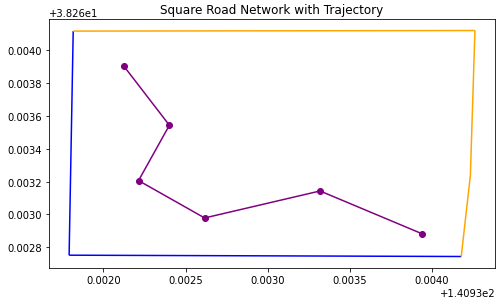
\includegraphics[width=1.2\linewidth]{square.png}
\caption{Square Example}
\label{square}
\end{minipage}
\hfill
\begin{minipage}[c]{0.4\linewidth}
    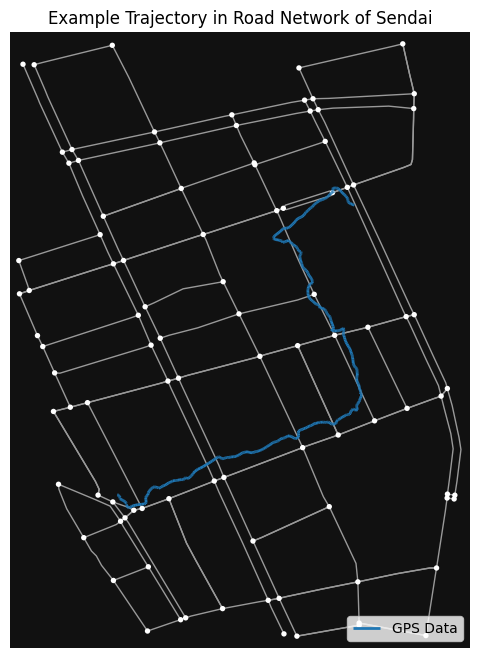
\includegraphics[scale=.43]{trajectoryandroads.png}
    \caption{Sendai Example}
    \label{sendai}
\end{minipage}%
\end{figure}







The dataset we used for evaluation of the electrical and harmonic oscillator methods was the \textit{Dataset for testing and training of map-matching algorithms} \cite{KCMMN}. This dataset was a good fit for the project because it included ground truths, despite only possessing GPS data. We were unable to apply the Wasserstein method to this data set due to issues discussed in \autoref{WassSection}.  Although we pre-processed the BDD100K open dataset provided by Berkeley for evaluation, it does not contain ground truths, so we were unable to utilize it for this project.  \cite{yuBDD100KDiverseDriving2020}. 

\subsection{Preprocessing Routes}

As the number of edges in a directed graph increases, the number of routes between two nodes grows at a rate similar to the factorial (and can be infinite if loops are allowed); moreover, the determination of all such routes is NP-hard. As a result, it is not sufficient to simply determine a suitable loss function and evaluate all possible routes. Finally, our loss functions are often expressed as integrals, so even once we have our routes, we need to interpolate each route so that the sum sufficiently approximates the integral. In practice, we do all this by restricting to a sub-graph, using an algorithm to obtain a restricted set of candidate routes, and then interpolating the resulting routes. We refer to these steps as preprocessing.

Of course, the preprocessing process need only be done once for a given dataset. That is, once we preprocess our graph with our trajectory, we can utilize the processed information for all of our algorithms. Furthermore, all the preprocessed information can readily be saved to disk, so for larger datasets, this need only be done once.

\subsubsection{Restricting to a Sub-graph}
\label{ssub:restrict-to-a-subgraph}

The method we use to restrict to a sub-graph is relatively simple. We choose a $k \in \Z_+$, and for each point $p_i$ in the trajectory, we find the set of $k$-nearest edges with their respective nodes (or all the possible edges, in the rare case that there are fewer than $k$ edges), denoted $E_{p_i}^k$. Our restricted sub-graph $\tilde{G}$ is then given by
\begin{align}
    \tilde{G} = \bigcup_{p_i} E_{p_i}^k.
\end{align}

Unlike $k$-nearest nodes, $k$-nearest neighbors are more computationally difficult. A $k$-d tree is not possible because we have to consider \textit{all} points around an edge. As a result, we are forced to rely on geometric tools to find this set. We do this by choosing an $r>0$ and creating a square of size $2r$ centered at each $p_i$, and finding the geometric intersection with the road network. If at a given point the square does not intersect at least $k$ edges, we double the value of $r$ and repeat the process, until we have found enough edges or we have doubled the value ten times. This method was inspired by the implementation of FMM \cite{YG}.

This method is quite inefficient. In the future, we hope to explore using mathematical geometric tools to better find our sub-graph.

\subsubsection{Obtaining Candidate Routes}
\label{ssub:obtaining-candidate-routes}

Once we have obtained our sub-graph $\tilde{G}$, we utilize a variant on Dijkstra`s algorithm to generate a list of short paths between our source and target. First we identify the source and target node on $\tilde{G}$ by finding the closest neighbor to $p_1$ and $p_n$. Then we follow the standard procedure of Dijkstra's algorithm by visiting the nodes connected to the route with lowest cost. Unlike Dijkstra's algorithm, we keep each route obtained, even if we have found a shorter route to get to the same intermediate node. We continue Dijkstra's algorithm until we have either enumerated every route or have obtained the number of routes desired. We do return the cost of each route as well, but we do not use this information in our algorithms-- the shortest route is not necessarily the best candidate route!

This method is a reasonably fast way to take a breadth-first search approach, but nevertheless is still quite slow. Furthermore, while Dijkstra's algorithm can be modified to allow multiple source and target nodes, we choose not to apply this as it would require us to generate many more candidate routes to ensure the true route is within our set.

There are some edge cases where this algorithm will fail. For one, if the number of nearest edges is not sufficiently high, the sub-graph will not be able to find any candidate route. In this situation one has to increase the number of candidate edges and start the algorithm from scratch-- which can be very computationally expensive. The algorithm is also not designed to handle routes where the same edge is traversed more than once; these cases are exceedingly rare, and so we did not find it necessary to modify the algorithm for this purpose.

This algorithm also is difficult to run in parallel. Conceptually, it should be possible to search multiple routes at once, but this requires a more robust task assignment process. We did not have the time to explore this option, and more importantly, it may not be worth it if better candidate route generation methods are available.

Despite these shortcomings, the candidate routes obtained are usually high quality. Unlike some data-driven implementations, we also know that when we find our optimal route, it will be a valid route.

\subsubsection{Candidate Route Interpolation}

The interpolation process is rather simple. Because our objects are Shapely geometries, we can interpolate each edge using Shapely's built-in interpolation. We choose constants $n_r,n_t \in \Z_+$ and interpolate each edge of the candidate route into $n_r$ segments and each edge of the trajectory into $n_t$ segments.

One concern is how to determine the constants $n_r$, $n_t$ a priori. We found that choosing $n_r \approx 100$ and $n_t \approx 10$ produced the best results; however, in the future we wish to implement a more dynamic approach which interpolates based on the relative density of the points.

Typically with simpler loss functions such as the electric method or harmonic oscillator method, increasing the interpolation points does not significantly increase computation time. However, in the case of the Wasserstein method, it had a big impact on computation time. Thus the optimal choice of $n_r$ and $n_t$ depend greatly on the method.

A shortcoming of this method is that it interpolates every edge equitably. This means that very small edges will have a high density of points, while a long edge will be more sparse. This may give an unfair weighting to small edges. In the future we wish to explore a dynamic choice of interpolation points based on the lengths of an edge.

\subsection{Wasserstein Distance Implementation}\label{WassSection}

Let $\{p_{i}\}$ be the set of trajectory points and discretize $A\in\CR_G$ into $m+1$ equal parts to obtain the set of  threshold points $V(A,m)\:=\{a_1,a_2,\ldots,a_m\}$. Then, from \autoref{IntroOfOT}, we know can find the Wasserstein distance by solving the following linear program
\begin{align}
\begin{aligned}
    & \text{minimize} 
        & \sum_{i=1}^n \sum_{j=1}^m d(p_i,a_j)\pi(p_i,a_j) & & \label{object func.1} \\
    & \text{subject to} 
        & \pi(p_i,a_j)\ge 0 & \qquad \text{for } i=1,2,\ldots,n,\, j=1,2,\ldots,m, \\
        & & \mu(p_i)=\sum_{j=1}^m \pi(p_i,a_j) & \qquad \text{for } i=1,2,\ldots,n, \\
        & & \nu(a_j)=\sum_{i=1}^n \pi(p_i,a_j) & \qquad \text{for } j=1,2,\ldots,m. 
\end{aligned}
\end{align}


After selecting $n,m$, we solve this linear program in python using the linprog command from Scipy's optimization package. The constraint matrix constructed will be size $(n+m) \times nm$, but only $2mn$ elements will be nonzero. Thus, the constraint matrix can be saved as a sparse matrix. For the computation, we remove one of the constraints, because the system is overdetermined as written. In contrast, it is likely that no  $d(p_i,a_j)$ will be zero. Therefore, for each candidate route, we must compute $nm$ distances. 


For the simple example of a trajectory contained in a square road network, see \autoref{wSquare}, the loss computed for each route is the Wasserstein distance. The chosen route in this instance is Route 1. We can see that the loss for Route 1 is smaller, and is the route we would have chosen to be correct through visual analysis. 
\begin{figure}[h!]
    \raggedleft
    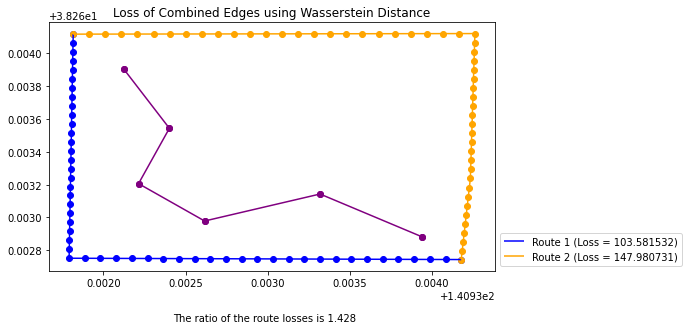
\includegraphics[scale=.5]{Wass.png}
    \caption{Wasserstein solution to the Square Example}
    \label{wSquare}
\end{figure}


In contrast, when we apply Wasserstein distance to the example of the Sendai map, the route that minimizes Wasserstein distance is longer and more complex than the true route. In figure \autoref{wSendai}, we see the route with minimal Wasserstein distance. Not only does it stray from the trajectory substantially, but it also contains a loop. At this time, we are unsure if this is an issue with the method itself or some implementation error. One obstacle to determining this is the computational time. Computing the Wasserstein distances on the set of candidate routes for the Sendai map alone can take several hours.

\begin{figure}[h!]
    \centering
    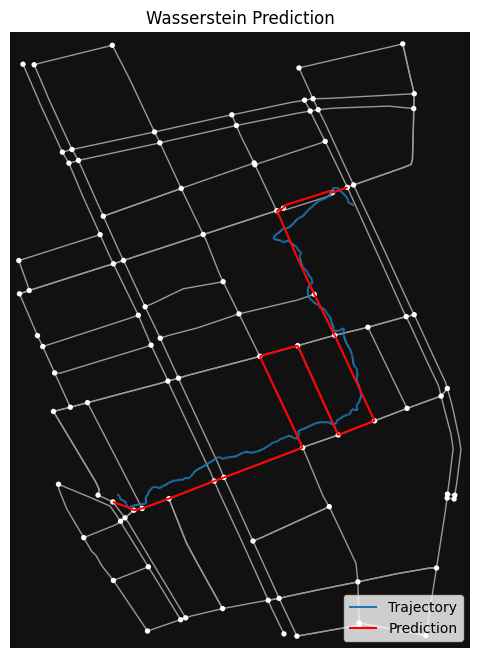
\includegraphics[scale =.3]{Jupyter Notebook LaTeX/wassersteinsendai.png}
    \caption{Wasserstein solution to the Sendai Example}
    \label{wSendai}
\end{figure}




\subsection{Electrical Method and Harmonic Oscillator Implementation}

In comparison, the electric method and harmonic oscillator are simpler to compute. Let $\textrm{Tr} = \left\{ p_i \right\}$ be the set of trajectory points and $A = \left\{q_i\right\}$ be the set of points along a candidate route. For each $p_i$ we determine the $k$-nearest neighbors from the set $\left\{q_i\right\}$; that is, for each $p_i$ we obtain a subset $\left\{q_j\right\}_{j \in 1,...,k}^{p_i} \subset \left\{ q_i \right\}$. Then we compute the sums:
\begin{align}
    E_\textrm{Tr}(A) &= \sum_{p_i} \sum_{j = 1}^k \frac{-1}{d(p_i,q_j)^2 + \eps} \quad& \text{(Electrical Method)}\\
    \textrm{Act}_\textrm{Tr} (A) &= \sum_{p_i} \sum_{j=1}^k d(p_i,q_j)^2 \quad& \text{(Harmonic Oscillator Method)}
\end{align}
where $0<\eps\ll 1$ is a small constant chosen to prevent divergence.

In particular, for the electric method, we choose $k = \# \left\{q_i\right\}$ (that is, we compare to all the points along the candidate route), and for the harmonic oscillator method, we choose $k = 1$ (that is, we only compare to the nearest neighbor). On one hand, choosing large $k$ means you take into account more of the polyline; however, points far away from the polyline may have a large influence on the loss. Typically this does not change the relative losses between two candidate routes, but it does make the losses numerically much closer-- and in extreme cases, we may lose this relative information due to floating point errors. Conversely, for small $k$ we are only considering the part of the candidate route most relevant to a given point; however, outliers in the trajectory may cause the loss of a candidate route to be lower than expected. Therefore, it is likely that the optimal value for $k$ lies somewhere in between. Of course, it is difficult to determine a priori what $k$ is appropriate for a given case.



%We compare the performance of our methods to Fast Map-Matching \cite{YG}.
    % \begin{itemize}
    %     \item point-to-curve method
    %     \item HMM, such as an extended Kalman filter (EKF) or Fast Map-Matching \cite{YG}
    %   % \item Fast Map-Matching \url{https://github.com/cyang-kth/fmm}.
    % \end{itemize}

\subsection{Evaluation (Error) Method} \label{Eval}
\label{sub:evaluation}

How do we measure the accuracy of our prediction? We use the following formula presented by Newson and Krumm \cite{newsonHiddenMarkovMap2009} to calculate the error:
$$\textrm{Err} = \frac{d_- + d_+}{d_0}$$ where $d_0$ is the length of the correct route, $d_-$ is the length the prediction erroneously subtracted from the ground truth, and $d_+$ is the length the prediction erroneously added outside the ground truth. See \autoref{fig:error-formula}.

\begin{figure}[ht]
    \centering
    \def\svgwidth{\linewidth}
    \input{error-formula.pdf_tex}
    \begin{align*}
	    d_0 &= \text{length of ground truth}\\
	    d_- &= \text{length of prediction route erroneously subtracted}\\
	    d_{+} &= \text{length of prediction route erroneously added}
    \end{align*}
    \caption{Error Formula by Newson and Krumm}
    \label{fig:error-formula}
\end{figure}

\subsection{Preliminary Results}

When tested on the dataset, we found that FMM had an error of 14.7\% on average \ref{fig:fmmerror}.

\begin{figure}
    \centering
    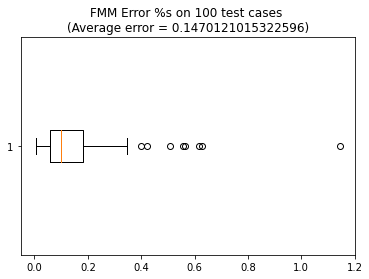
\includegraphics[scale=.5]{Jupyter Notebook LaTeX/fmmerror.png}
    \caption{FMM evaluated on the annotated dataset}
    \label{fig:fmmerror}
\end{figure}

Unfortunately, due to processing power and time constraints, we were unable to evaluate our algorithms on the entirety of the dataset. In particular, the preprocessing stage was too slow on the much larger networks to allow for testing. As a result we can only provide preliminary results for two of the methods \ref{fig:elec-error} \ref{fig:harm-osc-error}.


\begin{figure}[h!]
\begin{minipage}[c]{0.4\linewidth}
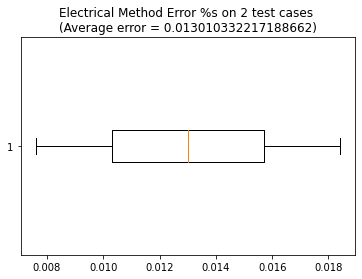
\includegraphics[scale=.55]{Jupyter Notebook LaTeX/electricerror.png}
\caption{Electric Method evaluated on annotated dataset}
\label{fig:elec-error}
\end{minipage}
\hfill
\begin{minipage}[c]{0.4\linewidth}
    \centering
    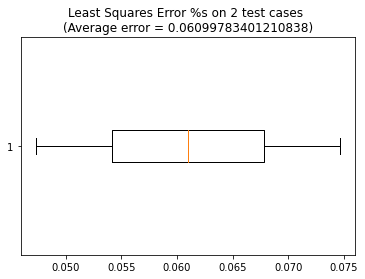
\includegraphics[scale=.55]{Jupyter Notebook LaTeX/leastsquareerror.png}
    \caption{Harmonic Oscillator Method evaluated on the annotated dataset}
    \label{fig:harm-osc-error}
\end{minipage}%
\end{figure}


% \begin{figure}
%     \centering
%     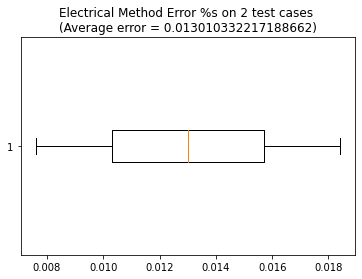
\includegraphics{Jupyter Notebook LaTeX/electricerror.png}
%     \caption{Electric Method evaluated on the annotated dataset}
%     \label{fig:elec-error}
% \end{figure}

% \begin{figure}
%     \centering
%     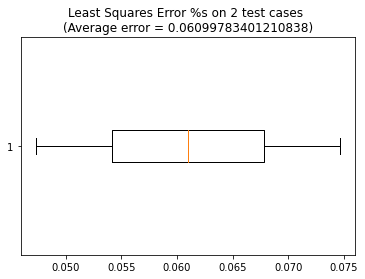
\includegraphics{Jupyter Notebook LaTeX/leastsquareerror.png}
%     \caption{Harmonic Oscillator Method evaluated on the annotated dataset}
%     \label{fig:harm-osc-error}
% \end{figure}

We anticipate that the geometric methods will perform more accurately than FMM on the dataset, but at the cost of (significantly) greater computation time.

\subsection{Computational Complexity}

We tested the computational complexity of the preprocessing stage and our methods. In particular, the preprocessing stage scales linearly with the number of candidate routes to find, but scales exponentially with the number of candidate edges provided \ref{fig:pre-comp-complex}. Both the Electric Method and the Harmonic Oscillator Method seem to scale linearly $\mathcal{O}(n)$ with the number of candidate routes \ref{fig:elec-comp-complex}\ref{fig:hom-comp-complex}. When the number of distance calculations were increased (i.e. more nodes in the candidate route and trajectory), runtime increased, but not significantly-- certainly slower than linear growth. Unfortunately, the Wasserstein method grew too rapidly when distance calculations were increased, and so a similar figure could not be produced for the method. We suspect that it scales as a polynomial of degree $>1$ with respect to distance calculations.

\begin{figure}
    \centering
    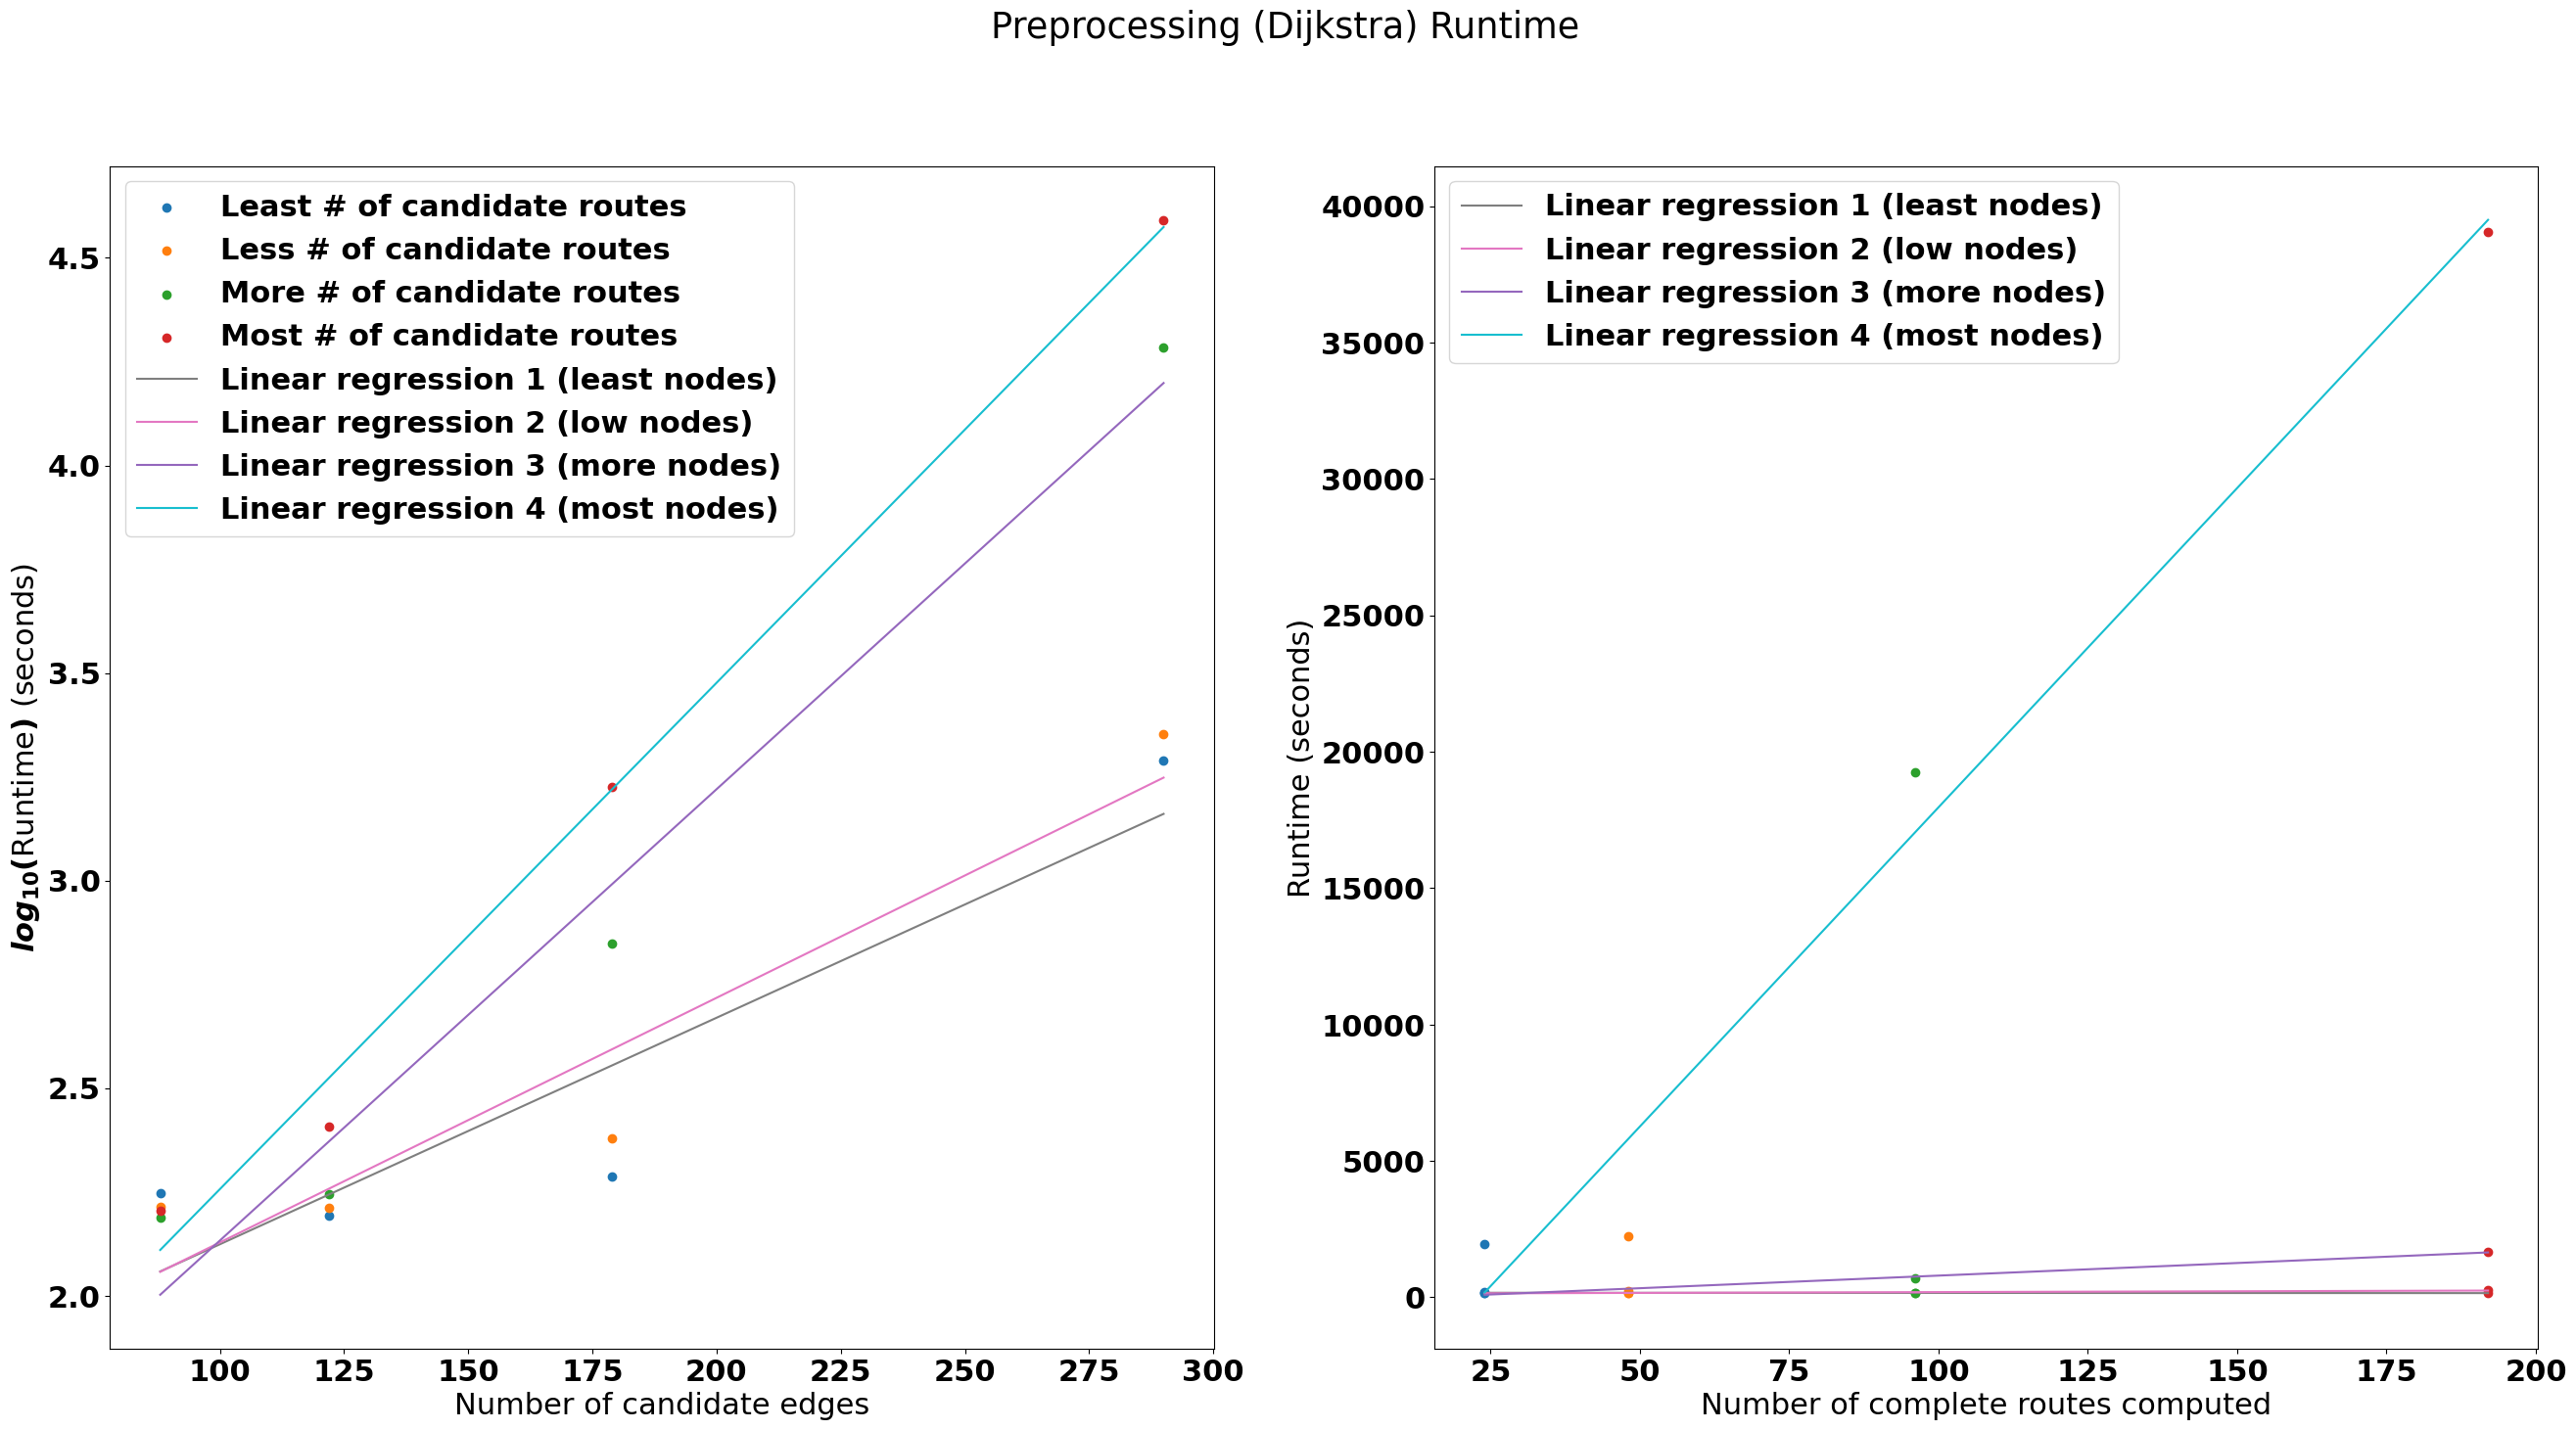
\includegraphics[scale = 0.25]{Jupyter Notebook LaTeX/preprocessing.png}
    \caption{Preprocessing Computation Runtimes}
    \label{fig:pre-comp-complex}
\end{figure}

\begin{figure}
    \centering
    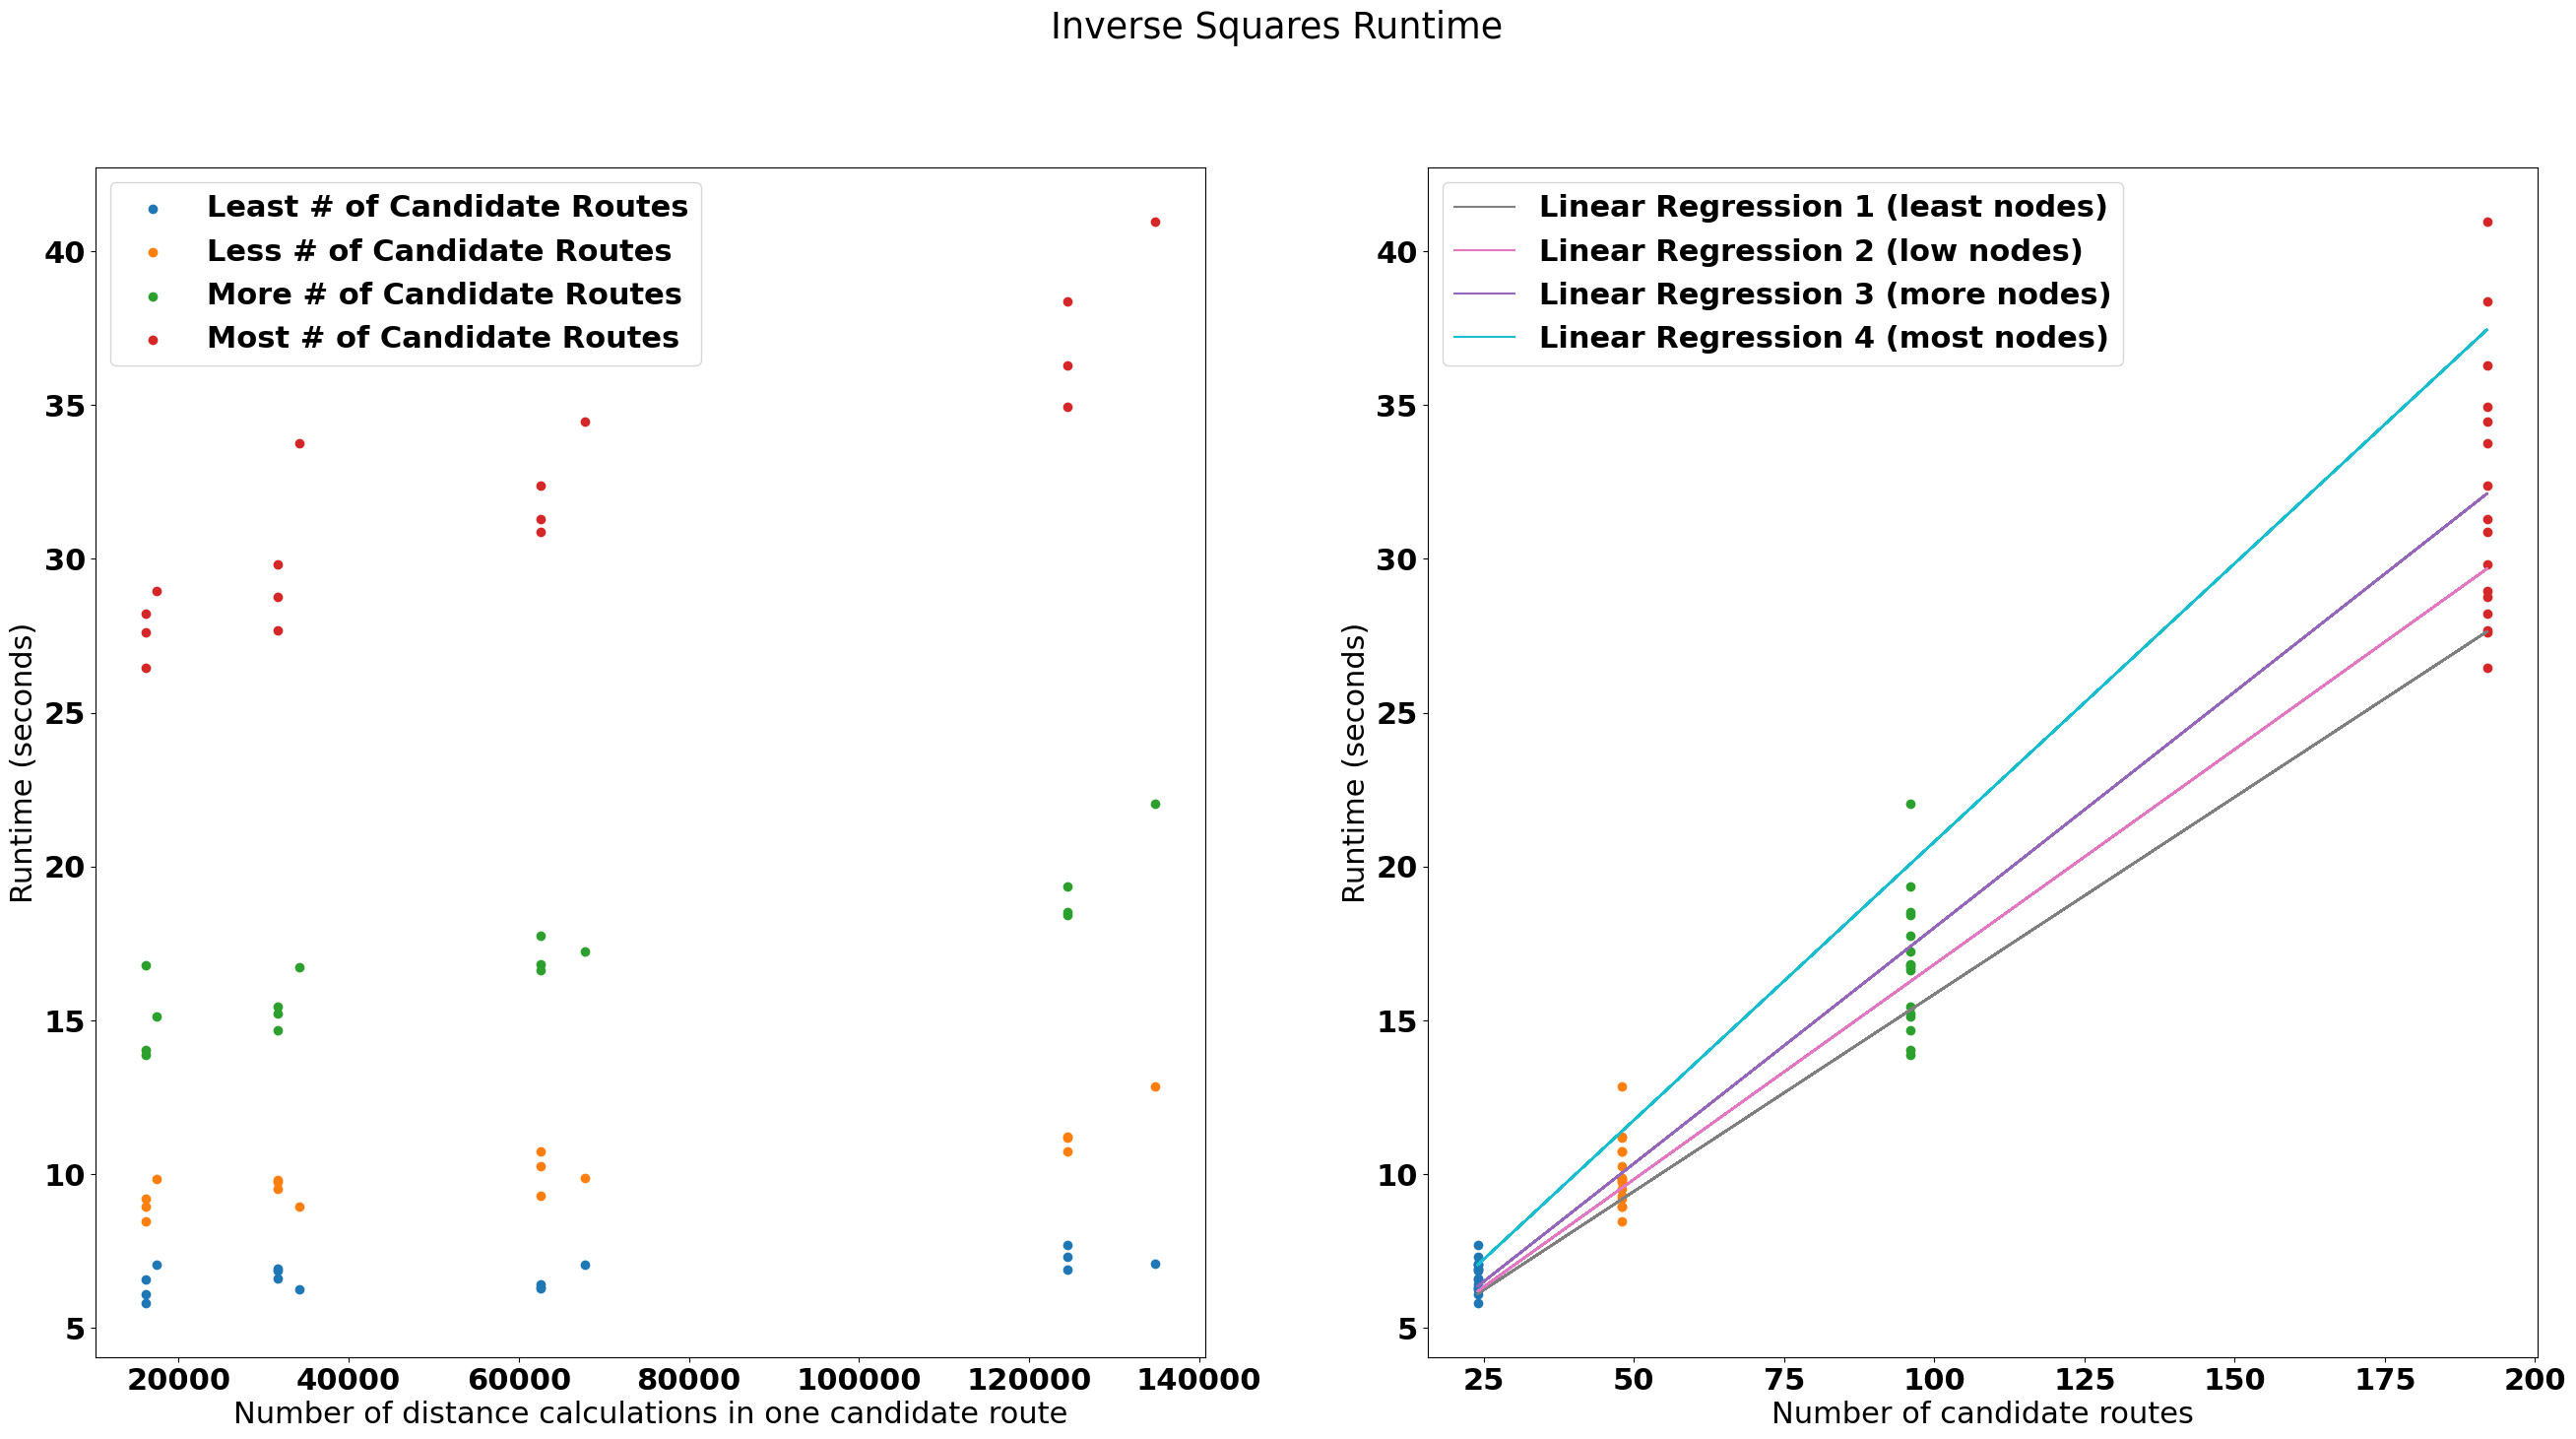
\includegraphics[scale = 0.25]{Jupyter Notebook LaTeX/complexity2.png}
    \caption{Electric Method Computation Runtimes}
    \label{fig:elec-comp-complex}
\end{figure}

\begin{figure}
    \centering
    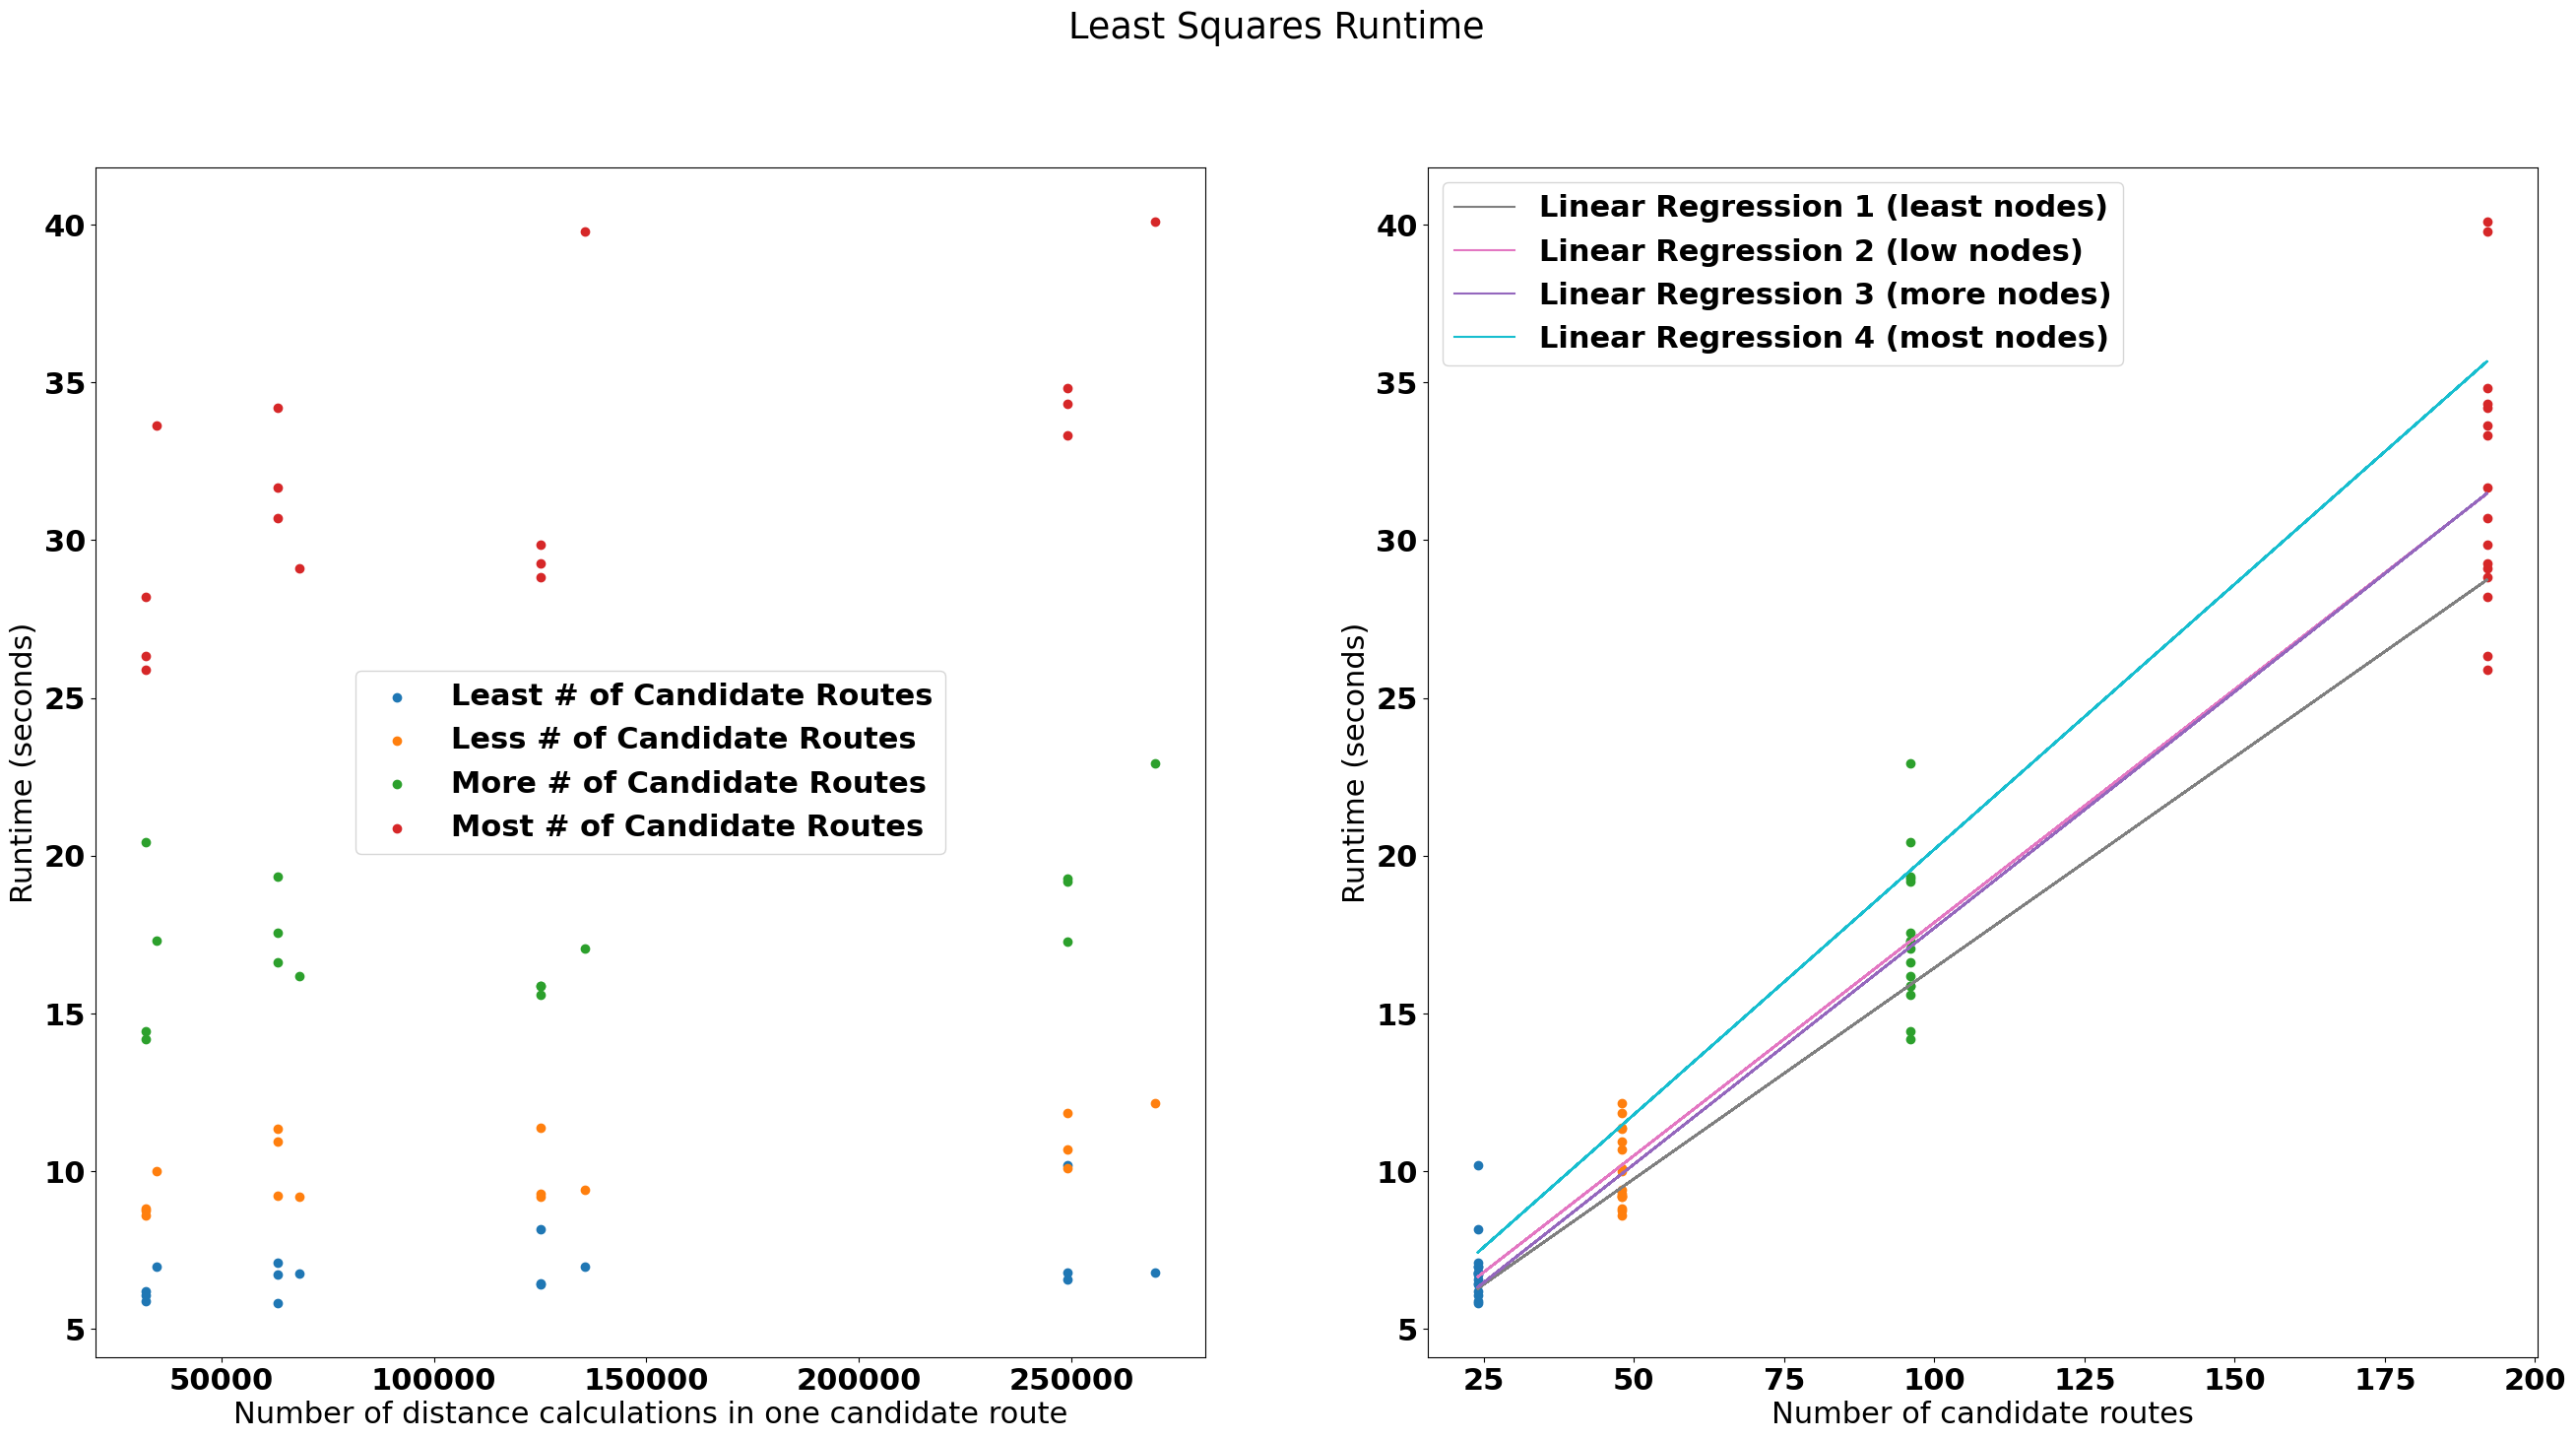
\includegraphics[scale = 0.25]{Jupyter Notebook LaTeX/complexity1.png}
    \caption{Harmonic Oscillator Method Computation Runtimes}
    \label{fig:hom-comp-complex}
\end{figure}

The metric algorithm framework can parallelize over the number of candidate routes, which significantly improves the computation complexity. It is unlikely that improvements can be made within the loss functions to parallelize further, as Electric Method and Harmonic Oscillator Method utilize array operations, and Wasserstein utilizes linear programming.

While candidate route generation has limited room for parallelization, one can easily parallelize the process across the entirety of the dataset. The simulators can also be easily run in parallel on the entirety of the dataset.

\subsection{Metric-based Algorithm Framework}

Because the basic formulation of our proposed map matching algorithms are all purely metric-based, we realized it was more efficient to write the algorithm in a modular capacity. This led to the creation of the generalized metric\_mm algorithm class.

To create a metric\_based map matching algorithm simulator, one first creates a loss function in one of two ways:

\begin{itemize}
    \item Providing simple interior and exterior functions which operate in stages on the distance arrays
    \item Providing a singular loss function which takes as arguments the candidate route distance array and the trajectory distance array.
\end{itemize}

Often it is simpler to provide the latter, but the former may be convenient in the case that one wishes to make small modifications to the loss function procedure in a systematic capacity.

If preprocessing has already been performed by another simulator, the interpolated candidate route nodes and trajectory can be provided directly.

The class then provides a preprocessing method if preprocessing has not already been performed. It's only required argument is a GeoDataFrame consisting of LineStrings of the trajectory (this can be generated from a sequence of points using a utility function provided in another module). If candidate routes are not provided, it applies the variant on Dijsktra's algorithm described in \ref{ssub:obtaining-candidate-routes}.

To run the simulator, one simply has to call the run method. This will return the best candidate route (and its loss) or the loss of all candidate routes depending on parameters passed.

\subsection{Data Fusion}
In addition to map matching, the Jupyter notebooks providing a framework for implementing and testing algorithms on driving datasets. One issue that pervades this field of research is the high variety in file formatting, and in particular, these formats are not well-suited for containing IMU data. Our notebooks provides a rudimentary fusion method to align asynchronous data and incorporates IMU data into a GeoDataFrame (which can be exported to GPX, GeoJSON, KML, etc.) in a sensible manner. In particular, this method can sample any discrete-time data such as speed, accelerometer, and gyroscope, and merge it with the GPS data sequence.

\subsection{Other Utilities}

In the process of creating this framework, several utility functions and classes have been provided. Within mm\_utils.py we provide functions such as:
\begin{itemize}
    \item Basic plotting methods
    \item An evaluation method to calculate error
    \item A method to create trajectory edges (LineStrings) from a sequence of coordinates (Points)
    \item A method which provides a road network from OSM (as a MultiDiGraph or GeoDataFrame) from the trajectory data only
    \item A method to find $k$ nearest points using $k$-d trees
    \item A method to find $k$ nearest edges using the method described in \ref{ssub:restrict-to-a-subgraph}
\end{itemize}

%The benefit these data types provide is being simple (human-readable and easy to convert from/to) and lightweight (quick to access and manipulate, and simple to compress). Moreover, it is easy to convert from these data types to others, unlike proprietary formats such as ESRI ShapeFile. Testing algorithms against datasets then reduces to formatting your inputs/outputs properly. This is designed for accessibility, so other students or researchers can experiment with their ideas and obtain results more easily.

\section{Future Work (Implementation)}

We briefly mention again improvements discussed in the previous section:
\begin{itemize}
    \item Modify $k$-nearest edge search with more efficient methods
    \item Modify or replace Dijsktra's algorithm for candidate route generation
    \item Investigate and improve upon Wasserstein method
\end{itemize}

\subsection{IMU Inclusion}

While IMU approaches were proposed theoretically, we did not have the time to include IMU information into our algorithm implementations. Currently the generalized metric-based map matching framework does not pass IMU data to the loss functions, but it is preserved in all the intermediate stages, so it should be simple to modify it so that the relevant data is passed along.

\subsection{Incomplete Map Matching}

One area of interest with map matching problems is incomplete maps. Our assumption is that our road network includes every possible path in reality. Of course, some older roads or even new roads may not be incorporated into our road network information. One direction of interest is then to explore if we can determine when roads are missing from our network based on the loss values along the trajectory.

\subsection{Extension to Higher Dimensions}

Including the $z$-axis into our implementation faces one major hurdle: OpenStreetMaps does not include elevation. Because this information is not included within our network, we cannot test our algorithms in $3$-space. One can circumvent this by merging elevation data from an external source. However, highways and roads are often not incorporated into these data sets, and so it is approximate at best. Instead, it is probably best to source network information from more detailed data sets, such as proprietary sources, but results can vary greatly depending on the region.\\

Fortunately, the Python framework developed is quite modular, so if one does have elevation data in their network and test data, it is easy to implement within our notebooks. Hopefully, with time, data sets such as OpenStreetMaps will gain detail, and this line of inquiry becomes more accessible to the scientific community.

\section{Conclusion}

We developed 3 new loss functions for solving the map-matching problem: Wasserstein, Electrical, and Harmonic Oscillator. Within each theoretical formulation, not only can we determine a route from distance information, but also by accounting for speed and direction information. For the Wasserstein distance method, this achieved through a perturbation of the probability measures on both the trajectory data and the threshold points on the candidate routes. For the harmonic oscillator, the speed and direction are incorporated through the momentum term of the Hamiltonian. Each method was also implemented in Python, but using only the distance information. The results for Wasserstein distance suggests either the formulation or the implementation requires more investigation. However, the electric and harmonic oscillators results are promising. Although their computational time is greater than that of FMM, in the experiments that we have run so far, the accuracy seems much improved.


\begin{appendices}

% \appendix
\setcounter{figure}{0}
\setcounter{table}{0}


\section{Geometric background of Wasserstein method} \label{appendix}

This section provides the geometric background of the Wasserstein method in \autoref{Wasserstein method}.
Wasserstein method is based on the concept of ``Ricci curvature of graph", which was introduced by \cite{Ol,LLY}.
This concept is a metric to measure the strength of cohesion between two vertices and has attracted attention as a new tool for graph analysis and has already been applied to real problems (\cite{JL,NLGGS,NLLG}, etc.).
We modified Ricci curvature of graphs to quantify the ``strength of cohesion" between the trajectory and each route.

\subsection{Ricci curvature of graphs} \label{subappendix:graph}

In this section, we briefly describe the Ricci curvature of graphs.
We consider a weighted graph.
Denote the weight of edge $e$ as $w_e$.
In this case, the node degree $d_x$ of vertex $x$ is $d_x=\sum_{y\sim x}w_{xy}$.
We call a graph with a weight of $1$ on all edges a \emph{combinatorial graph}.
First, we introduce a transition probability measure on a node.
In this section, we use $x,y$ as symbols that denote nodes.

\begin{definition}[Random walk with idleness parameter $\eps\in\text{[0,1]}$] \label{random walk}
For each node $x\in V$ and $\eps\in[0,1]$, we define a random walk $\rwx$ as follows: \vspace{-6mm}
\begin{center}
\[ \dis \rwx(y) \:=
\begin{cases}
1-\eps & (y=x) , \vspace{1mm} \\
\eps\cdot\frac{w_{xy}}{d_x} & (y\sim x) , \vspace{1mm} \\
0 & (\text{otherwise}) .
\end{cases}\]
\end{center} 
\end{definition}

The Ricci curvature with idleness parameter $\eps$ is defined as follows.

\begin{definition}[$\eps$-Ollivier--Ricci curvature; \cite{Ol,LLY}] \label{eps-curv}
Let $\eps\in[0,1]$.
The \emph{$\eps$-Ollivier--Ricci curvature $\kexy$} between two nodes $x,y\in V$ is defined as 
\begin{align*}
\kexy\:=1-\frac{\wxy}{d(x,y)}.
\end{align*}
\end{definition}

When $\eps=0$, $\K(0;x,y)=0$ for any nodes $x,y$.
Then, in \cite{LLY}, they defined a curvature as the (right) limit $\lim_{\eps\dto0}\kexy/\eps$ instead of simply assigning $\eps=0$ (\autoref{LLY-curv}).
To confirm the existence of this limit, the following two lemmas were shown.

\begin{lemma}[{\cite[Lemma 2.2]{LLY}}] \label{LLY-bdd}
For any $\eps\in[0,1]$ and $x,y\in V$, we have
\begin{align*}
|\kexy|\leq\frac{2\eps}{d(x,y)}. %\label{ineq:LLY-bdd}
\end{align*}
\end{lemma}

\begin{lemma}[{\cite[Lemma 2.1]{LLY}}] \label{LLY-concavity}
For two vertices $x,y$, $\K(\eps;x,y)$ is concave in $\eps\in[0,1]$.
\end{lemma}

The shape of $\K(\eps;x,y)$ in $\eps\in[0,1]$ was later examined in more detail.

\begin{thm}[{\cite[Theorem 3.4]{BCLMP}, \cite[Theorem 3.2]{CK}}] \label{3-pieces}
For any connected, locally finite and simple graph $G=(V,E)$ and any of its nodes $x,y$, the function $\varphi:\eps\mapsto\kexy$ is concave and piecewise linear on $[0,1]$.
Moreover, the number of its partitions is at most $3$.
In particular, $\varphi(\eps)\:=\kexy/\eps$ is constant for $\eps$ sufficiently close to $0$.
\end{thm}

In \cite{BCLMP}, the case of $x\sim y$ was shown, then in \cite{CK} established the general case by using the Kantorovich duality of $W_1$ distance.

From \autoref{LLY-bdd} and \autoref{LLY-concavity}, we can see the existence of the (right) limit $\lim_{\eps\dto0}\kexy/\eps$.

\begin{definition}[LLY--Ricci curvature; \cite{LLY}] \label{LLY-curv}
We define the \emph{LLY--Ricci curvature} $\kxy$ between two nodes $x,y\in V$ as
\begin{align*}
\kxy\:=\lim_{\eps\dto0}\frac{\kexy}{\eps}. 
\end{align*}
\end{definition}

Although LLY--Ricci curvature $\kxy$ is a limit value, it can be obtained by linear programming (\cite{CKLLS}) thanks to \autoref{3-pieces}.
Moreover, the Graph Curvature Calculator\footnote{\url{https://www.mas.ncl.ac.uk/graph-curvature/}
On this page, you can select from the tabs in the lower left corner to calculate various types of curvatures.
The tab ``Lin--Lu--Yau Curvature" allows you to calculate the curvatures used in this study.
Remark that these are calculated on \textbf{unweighted graphs}, and the following discussion considers \textbf{weighted graphs}.} 
has been developed to calculate LLY--Ricci curvature of each edge of a graph by inputting node and edge information.

\subsection{``Ricci curvature" between the trajectory and route} \label{subappendix:map-matching}

According to \autoref{LLY-curv}, we introduce a ``curvature" between the trajectory and each route.
It is this quantity that determines which routes the trajectory is closer to.

The denominator $d(x,y)$ used in the \autoref{LLY-curv} (i.e. \autoref{eps-curv}) was the distance between the two vertices $x,y$ of the target.
In this setting, the target to be measured is not two vertices but two ``sets of vertices".
Therefore, it is necessary to first consider what the quantity corresponding to $d(x,y)$ should be in this setting.
In conclusion, we adopt $W_1(\mu_\mathbf{p}, \nu_A)$ (with respect to the route $A$) as described in the midterm presentation.
This is because $W_1(\mu_\mathbf{p}, \nu_A)$ was quantifying the distance between the trajectory and route using only the location information of the trajectory.
We next need to consider the amount of the numerator of \autoref{eps-curv}.
In the idea of \autoref{LLY-curv}, they perturbed the Dirac measures\footnote{
Here, notice that $d(x,y)$ can be transformed to $d(x,y)=W_1(\dex,\dey)$ and $\mu_x^0=\dex$, $\mu_y^0=\dey$.
This means that the fraction \autoref{eps-curv}: $W_1(\mu_x^\eps,\mu_y^\eps)/W_1(\dex,\dey)$ measures the fundamental probability measures $\dex,\dey$ in the denominator and the $\eps$-perturbations $\mu_x^\eps,\mu_y^\eps$ of them in the numerator, with $W_1$ between them, respectively.}
at $x,y$ by $\eps$ along the graph structure.
In the setting of Wasserstein method (\autoref{input:tra&time}), the vertices of the local road network are only the trajectory and the divided points $\{a_1,\ldots,a_m,b_1,\dots,b_m\}$ of each route $A$ and $B$, and thus it is a problem of \textbf{how to introduce the edges}.
Note that we define the transition probabilities for routes as \textbf{combinatorial graphs}.
Then, we consider introducing \textbf{weighted edges} using the input speed and direction at each trajectory point and we set up and defined them as described in \autoref{S&D}.

Now that $\eps$-perturbation measures have been defined, we can define the ``curvature" between the trajectory and routes as in \autoref{eps-curv} and \autoref{LLY-curv}.
In the following, we will write about route $A$ only, since the definition is the same for both routes $A$ and $B$.

\begin{definition}[$\eps$-Ricci curvature between the trajectory and route]
Let $\eps\in[0,1]$.
The \emph{$\eps$-Ricci curvature} $\kepa$ between the trajectory $\mathbf{p}$ and route $A$ is defined as: 
\begin{align}
    \kepa \:= 1-\frac{W_1(\mu_{\mathbf{p},A}^\eps,\nu_A^\eps)}{W_1(\mu_\mathbf{p},\nu_A)}. \label{eq:kepa}
\end{align}
\end{definition}

We next want to prove the corresponding properties for \autoref{LLY-bdd} and \autoref{3-pieces}.
However, we prove only the concavity of the function $\eps\mapsto\kepa$ corresponding to \autoref{LLY-concavity} (\autoref{kepa-concavity}) because the piecewise linearity of $h$ like \autoref{3-pieces} is not yet clearly known (see also \autoref{Wasserstein-FP}).

\begin{proposition}[$\eps$-boundedness of $\kepa$] \label{eps-bounded}
For any $\eps\in[0,1]$, we have
\begin{align*}
    \abs{\kepa} \le \frac{2\eps}{W_1(\mu_\mathbf{p},\nu_A)}. 
\end{align*}
\end{proposition}

\begin{proof}
By the triangle inequality of $W_1$, we obtain
\begin{align*}
    W_1(\mu_{\mathbf{p},A}^\eps,\nu_A^\eps) 
    &\le W_1(\mu_{\mathbf{p},A}^\eps,\mu_\mathbf{p}^0) + W_1(\mu_{\mathbf{p},A}^0,\nu_A^0) + W_1(\nu_A^0,\nu_A^\eps)
    = W_1(\mu_{\mathbf{p},A}^0,\nu_A^0) + 2\eps
    = W_1(\mu_\mathbf{p},\nu_A) + 2\eps, \\
    W_1(\mu_{\mathbf{p},A}^\eps,\nu_A^\eps) 
    &\ge W_1(\mu_{\mathbf{p},A}^0,\nu_A^0) - W_1(\mu_{\mathbf{p},A}^0,\mu_{\mathbf{p},A}^\eps) - W_1(\nu_A^0,\nu_A^\eps)
    = W_1(\mu_{\mathbf{p},A}^0,\nu_A^0) - 2\eps
    = W_1(\mu_\mathbf{p},\nu_A) - 2\eps.
\end{align*}
This implies the following:
\begin{align*}
    -\frac{2\eps}{W_1(\mu_\mathbf{p},\nu_A)} \le \kepa 
    \:= 1-\frac{W_1(\mu_{\mathbf{p},A}^\eps,\nu_A^\eps)}{W_1(\mu_\mathbf{p},\nu_A)} \le \frac{2\eps}{W_1(\mu_\mathbf{p},\nu_A)}.
\end{align*}
\end{proof}

\begin{proposition}[Concavity of $\kepa$] \label{kepa-concavity}
The function $h:[0,1]\ni\eps\mapsto\kepa\in\R$ is concave.
\end{proposition}

\begin{proof}
Let $\eps_1,\eps_2,\eps_3$ be $0\le\eps_1<\eps_2<\eps_3\le1$ and $t\:=(\eps_3-\eps_2)/(\eps_3-\eps_1)$.
Then, $\eps_2=t\eps_1+(1-t)\eps_3$ holds.
We show that 
\begin{align}
    \K(\eps_2;\mathbf{p},A) \ge t\K(\eps_1;\mathbf{p},A) + (1-t)\K(\eps_3;\mathbf{p},A) \label{ineq:kepa-concavity}
\end{align}
holds.
First, we show the following. \vspace{2mm} \\
\underline{\textbf{Claim}} 
Let $\pi_j$ be the optimal coupling between $\mu_{\mathbf{p},A}^{\eps_j}$ and $\nu_A^{\eps_j}$, with respect to $j=1,3$.
Then, $\pi_2\:=t\pi_1+(1-t)\pi_3$ is a coupling between $\mu_{\mathbf{p},A}^{\eps_2}$ and $\nu_A^{\eps_2}$.
\vspace{1mm} \\
\underline{\textit{Proof of \textbf{Claim}}}
$ $\newline
By the definition of $\pi_2$, we obtain 
\begin{align}
    \sum_{v_1\in V}\pi_2(v_1,v_2)
    &= t\sum_{v_1\in V}\pi_1(v_1,v_2) + (1-t)\sum_{v_1\in V}\pi_3(v_1,v_2)
    = t\nu_A^{\eps_1}(v_2) + (1-t)\nu_A^{\eps_3}(v_2) \notag \\
    &= t\cdot\frac{1}{m}\sum_{a\in V(A)}\nu_a^{\eps_1}(v_2) + (1-t)\cdot\frac{1}{m}\sum_{a\in V(A)}\nu_a^{\eps_3}(v_2) 
    \label{nu-coupling}, \\
    \sum_{v_2\in V}\pi_2(v_1,v_2)
    &= t\sum_{v_2\in V}\pi_1(v_1,v_2) + (1-t)\sum_{v_2\in V}\pi_3(v_1,v_2)
    = t\mu_{\mathbf{p},A}^{\eps_1}(v_1) + (1-t)\mu_{\mathbf{p},A}^{\eps_3}(v_1) \notag \\
    &= t\cdot\frac{1}{n}\sum_{p\in \mathbf{p}}\mu_{p,A}^{\eps_1}(v_1) + (1-t)\cdot\frac{1}{n}\sum_{p\in \mathbf{p}}\mu_{p,A}^{\eps_3}(v_1). \label{mu-coupling}
\end{align}
It is sufficient to check that the right hand side of \eqref{nu-coupling} and \eqref{mu-coupling} coincide with $\nu_A^{\eps_2}(v_2)$ and $\mu_{\mathbf{p},A}^{\eps_2}(v_1)$, respectively. \\
\underline{\eqref{nu-coupling}}
$\rm(\hspace{.18em}i\hspace{.18em})$ 
In the case of $v_2\in V(A)$: it holds that
\begin{align*}
    \eqref{nu-coupling} = t\cdot\frac{1}{m}(1-\eps_1) + (1-t)\cdot\frac{1}{m}(1-\eps_3)
    = \frac{1}{m}(1-\eps_2) = \frac{1}{m}\sum_{a\in V(A)}\nu_a^{\eps_2}(v_2) = \nu_A^{\eps_2}(v_2).
\end{align*}
$\rm(\hspace{.08em}ii\hspace{.08em})$ 
In the case of $v_2\in \mathbf{p}$: it holds that
\begin{align*}
    \eqref{nu-coupling} 
    = t\cdot\frac{1}{m}\bigg(\eps_1\cdot\frac{1}{n}\bigg)\cdot m + (1-t)\cdot\frac{1}{m}\bigg(\eps_3\cdot\frac{1}{n}\bigg)\cdot m
    = \frac{1}{m}\bigg(\eps_2\cdot\frac{1}{n}\bigg)\cdot m = \frac{1}{m}\sum_{a\in V(A)}\nu_a^{\eps_2}(v_2) = \nu_A^{\eps_2}(v_2).
\end{align*}
$\rm(i\hspace{-.08em}i\hspace{-.08em}i)$ 
In the case of $v_2\in V(B)$: it holds that $\eqref{nu-coupling} = 0 = \nu_A^{\eps_2}(v_2)$. \vspace{1mm} \\
\underline{\eqref{mu-coupling}}
$\rm(i\hspace{-.08em}v\hspace{-.06em})$ 
In the case of $v_1\in \mathbf{p}$: it holds that
\begin{align*}
    \eqref{mu-coupling} = t\cdot\frac{1}{n}(1-\eps_1) + (1-t)\cdot\frac{1}{n}(1-\eps_3)
    = \frac{1}{n}(1-\eps_2) = \frac{1}{n}\sum_{p\in \mathbf{p}}\mu_{p,A}^{\eps_2}(v_1) = \mu_{\mathbf{p},A}^{\eps_2}(v_1).
\end{align*}
$\rm(\hspace{.06em}v\hspace{.06em})$ 
In the case of $v_1\in V(A)$: it holds that
\begin{align*}
    \eqref{mu-coupling} 
    &= t\cdot\frac{1}{n}\sum_{p\in\mathbf{p}}\Bigg(\eps_1\cdot\frac{1+w_p(v_1)}{m+1}\Bigg) + (1-t)\cdot\frac{1}{n}\sum_{p\in\mathbf{p}}\Bigg(\eps_3\cdot\frac{1+w_p(v_1)}{m+1}\Bigg)
    = \frac{1}{n}\sum_{p\in\mathbf{p}}\Bigg(\eps_2\cdot\frac{1+w_p(v_1)}{m+1}\Bigg) \\
    &= \frac{1}{n}\sum_{p\in\mathbf{p}}\mu_{p,A}^{\eps_2}(v_2) = \mu_{\mathbf{p},A}^{\eps_2}(v_2).
\end{align*}
$\rm(\hspace{-.06em}v\hspace{-.08em}i)$ 
In the case of $v_1\in V(B)$: it holds that 
\begin{align*}
    \eqref{mu-coupling} 
    &= t\cdot\frac{1}{n}\sum_{p\in\mathbf{p}}\Bigg(\eps_1\cdot\frac{w_p(v_1)}{m+1}\Bigg) + (1-t)\cdot\frac{1}{n}\sum_{p\in\mathbf{p}}\Bigg(\eps_3\cdot\frac{w_p(v_1)}{m+1}\Bigg)
    = \frac{1}{n}\sum_{p\in\mathbf{p}}\Bigg(\eps_2\cdot\frac{w_p(v_1)}{m+1}\Bigg) \\
    &= \frac{1}{n}\sum_{p\in\mathbf{p}}\mu_{p,A}^{\eps_2}(v_2) = \mu_{\mathbf{p},A}^{\eps_2}(v_2).
\end{align*}
This concludes the proof of \textbf{Claim}. $\blacksquare$

\vspace{2mm}
From \textbf{Claim}, we obtain 
\begin{align*}
    W_1(\mu_{\mathbf{p},A}^{\eps_2},\nu_A) &\le \sum_{v_1,v_2\in V}\pi_2(v_1,v_2)d(v_1,v_2)
    = t\sum_{v_1,v_2\in V}\pi_1(v_1,v_2)d(v_1,v_2) + (1-t)\sum_{v_1,v_2\in V}\pi_3(v_1,v_2)d(v_1,v_2) \\
    &= tW_1(\mu_{\mathbf{p},A}^{\eps_1},\nu_A) + (1-t)W_1(\mu_{\mathbf{p},A}^{\eps_3},\nu_A).
\end{align*}
This yields the following:
\begin{align*}
    \K(\eps_2;\mathbf{p},A) 
    &\:= 1-\frac{W_1(\mu_{\mathbf{p},A}^{\eps_2},\nu_A^{\eps_2})}{W_1(\mu_\mathbf{p},\nu_A)}
    \ge t\Bigg( 1-\frac{W_1(\mu_{\mathbf{p},A}^{\eps_1},\nu_A^{\eps_1})}{W_1(\mu_\mathbf{p},\nu_A)} \Bigg)
    + (1-t)\Bigg( 1-\frac{W_1(\mu_{\mathbf{p},A}^{\eps_3},\nu_A^{\eps_3})}{W_1(\mu_\mathbf{p},\nu_A)} \Bigg) \\
    &= t\K(\eps_1;\mathbf{p},A) + (1-t)\K(\eps_3;\mathbf{p},A).
\end{align*}
This proves \eqref{ineq:kepa-concavity}.
\end{proof}

\begin{definition}[Ricci curvature between the trajectory and route]
The existence of the value of the limit $\lim_{\eps\dto0}\kepa/\eps$ 
is guaranteed by \autoref{eps-bounded} and \autoref{kepa-concavity}.
We define this value as \emph{Ricci curvature} $\kpa$ between the trajectory and route $A$:
\begin{align*}
    \kpa \:= \lim_{\eps\dto0} \frac{\kepa}{\eps}.
\end{align*}
\end{definition}

\begin{observation}
We determined the route with the smallest \eqref{W/W} to be the output as the true route.
Note that if \eqref{eq:S&D} holds, then we obtain
\begin{align*}
\K(\eps;\mathbf{p},A) 
\:= 1- \frac{W_1(\mu_{\mathbf{p},A}^{\eps},\nu_A^{\eps})}{W_1(\mu_\mathbf{p},\nu_A)} 
< 1- \frac{W_1(\mu_{\mathbf{p},A}^{\eps},\nu_A^{\eps})}{W_1(\mu_\mathbf{p},\nu_A)}
\eqqcolon \K(\eps;\mathbf{p},B).
\end{align*}
Therefore, the Wasserstein method is a method that outputs the route with the largest Ricci curvature with the trajectory as the true route.
\end{observation}

\begin{remark} \label{piecewise linear?}
As mentioned in \autoref{Wasserstein-FP}, we have not shown the piecewise linearity like \autoref{3-pieces} in LLY--Ricci curvature yet.
\end{remark}

\begin{remark}
This value may require modifications in the way the weights (\autoref{s&d-weight}) are assigned, as we have not yet calculated the concrete examples.
\end{remark}

\end{appendices}




\begin{small}
\bibliographystyle{unsrt}
% \bibliography{bibliography} 
\begin{thebibliography}{YCWXCLMD}
\bibitem[BCLMP]{BCLMP} D. P. Bourne, D. Cushing, S. Liu, F. M\"{u}nch and N. Peyerimhoff, \textit{Ollivier-Ricci idleness functions of graphs}, SIAM J. Discrete Math. \textbf{32}(2) (2018), 1408--1424.
\bibitem[BK]{BK}  D. Bernstein and A. Kornhauser, \textit{An introduction to map-matching for personal navigation assistants}, (1996).
%\url{http://www.njtude.org/reports/mapmatchintro.pdf}
\bibitem[CK]{CK} D. Cushing and S. Kamtue, \textit{Long-scale Ollivier Ricci curvature of graphs}, Anal. Geom. Metr. Spaces. \textbf{7}(1) (2019), 22--44. 
\bibitem[CKLLS]{CKLLS} D. Cushing, R. Kangaslampi, V. Lipi\"{a}inen, S. Liu and G. W. Stagg, \textit{The Graph Curvature Calculator and the curvatures of cubic graphs}, Exp. Math. (2019), 13pp. \\
\url{https://doi.org/10.1080/10586458.2019.1660740}
\bibitem[CXHZ]{CXHZ} P. Chao,  Y. Xu,  W. Hua and X. Zhou, \textit{A survey on map-matching algorithms}, Springer, Cham. (2020).
\bibitem[FG]{FG} A. Figalli and F. Glaudo, \textit{An invitation to optimal transport, Wasserstein distances, and gradient flows}, EMS Textbooks in Mathematics. EMS Press (2021).
\bibitem[GH]{GH} GraphHopper Github Repository, \url{https://github.com/graphhopper/graphhopper}.
\bibitem[JL]{JL} J. Jost and S. Liu, \textit{Ollivier's Ricci Curvature, Local Clustering and Curvature-Dimension Inequalities on Graphs},  Discrete Comput. Geom. \textbf{51}(2) (2014), 300--322.
\bibitem[Jo]{Jo} J. Jost, \textit{Riemannian geometry and geometric analysis}, $7$th edn. Springer, Berlin (2017).
%\bibitem[KCMMN]{KCMMN} M. KubiCka, A. Cela, P. Moulin, H. Mounier and S. I. Niculescu, \texit{Dataset for testing and training of map-matching algorithms,} 2015 IEEE Intelligent Vehicles Symposium (IV), 2015, pp. 1088-1093, doi: 10.1109/IVS.2015.7225829.
\bibitem[KCMMN]{KCMMN} M. Kubi\u cka, A. Cela, P. Moulin, H. Mountier and S. I. Niculescu, \textit{Dataset for testing and training of map-matching algorithms}, In 2015 IEEE Intelligent Vehicles Symposium (IV), 1088--1093 (2015).
\bibitem[LLY]{LLY} Y. Lin, L. Lu and S.-T. Yau, \textit{Ricci curvature of graphs}, Tohoku Math. J. (2) \textbf{63}(4) (2011), 605--627.
\bibitem[LSG]{LSG} X. Li, Y. Shi and I. Gutman, \textit{Graph energy}, Springer, New York. (2012).
%\bibitem[MW]{MW} F. M\"unch and R. K. Wojciechowski, \textit{Ollivier Ricci curvature for general graph Laplacians: heat equation, Laplacian comparison, non-explosion and diameter bounds}, Adv. Math. 356 (2019), 106759, 45pp.
\bibitem[NK]{newsonHiddenMarkovMap2009} P. Newson and J. Krumm, \textit{Hidden Markov map matching through noise and sparseness}, In Proceedings of the 17th ACM SIGSPATIAL international conference on advances in geographic information systems, 336--343 (2009). 
%Proceedings of the 17th ACM SIGSPATIAL International Conference on Advances in Geographic Information Systems - GIS ’09, 336. %https://doi.org/10.1145/1653771.1653818
\bibitem[NLGGS]{NLGGS} C.-C. Ni, Y.-Y. Lin, J. Gao, X. D. Gu and E. Saucan, \textit{Ricci Curvature of the Internet Topology}, In: IEEE Conference on Computer Communications. (2015), 2758--2766.
\bibitem[NLLG]{NLLG} C.-C. Ni, Y.-Y. Lin, F. Luo and J. Gao, \textit{Community Detection on Networks with Ricci Flow}, Sci Rep \textbf{9}, 9984 (2019), 12pp. \\
\url{https://doi.org/10.1038/s41598-019-46380-9}
\bibitem[Ol]{Ol}  Y. Ollivier, \textit{Ricci curvature of Markov chains on metric spaces}, J. Funct. Anal. \textbf{256}(3) (2009), 810--864.
\bibitem[QON]{QON} M. A. Quddus, W. Y. Ochieng and R. B. Noland. \textit{Current map-matching algorithms for transport applications: State-of-the art and future research directions}, Transportation research part $c$: Emerging technologies, \textbf{15}(5), 312--328 (2007).
\bibitem[QOZN]{QOZN} M. A. Quddus, W. Y. Ochieng, L. Zhao and  R. B. Noland, \textit{A general map-matching algorithm for transport telematics applications}, GPS Solutions \textbf{7}, 157--167 (2003). 
%10.1007/s10291-003-0069-z. 
\bibitem[Sa]{Sa} F. Santambrogio, \textit{Optimal transport for applied mathematicians. Calculus of variations, PDEs, and modeling}, Progress in Nonlinear Differential Equations and their Applications, Birkh\"{a}user/Springer, Cham. (2015).
\bibitem[Vi]{Vi} C. Villani, \textit{Optimal Transport. Old and New}, Springer-Verlag. (2008).
\bibitem[YG]{YG} C. Yang and G. Gid\' ofalvi, \textit{Fast map matching, an algorithm for integrating a hidden Markov model with precomputation}, International Journal of Geographical Information Science. Taylor \& Francis, \textbf{32}(3), 547--570 (2018).
\bibitem[YCWXCLMD]{yuBDD100KDiverseDriving2020} F. Yu, H. Chen, X. Wang, W. Xian, Y. Chen, F. Liu, V. Madhavan and T. Darrell, \textit{BDD100K: A Diverse Driving Dataset for Heterogeneous Multitask Learning}, In Proceedings of the IEEE/CVF conference on computer vision and pattern recognition, 2636--2645 (2020).
%(arXiv:1805.04687). arXiv.
\end{thebibliography}
\end{small}








\end{document}
